\documentclass[twoside,11pt,openright]{report}

\usepackage[american]{babel}
\usepackage{a4}
\usepackage{latexsym}
\usepackage{amssymb}
\usepackage{amsmath}
\usepackage{epsfig}
\usepackage[T1]{fontenc}
\usepackage{lmodern}
\usepackage[labeled]{multibib}
\usepackage{color}
\usepackage{datetime}
\usepackage{epstopdf} 
\usepackage[hidelinks]{hyperref}
\usepackage{algorithm}
\usepackage{algpseudocode}
\usepackage{tipa}
\usepackage{subcaption}
\usepackage{mathtools}
\usepackage{amsthm}
\usepackage{verbatim}
\usepackage{multicol}
\usepackage{mathtools}
\usepackage{moreverb}
\usepackage{tablefootnote}
\usepackage{placeins}
\usepackage{chngpage}
\usepackage{xfrac}
\usepackage[toc,page]{appendix}
\usepackage[utf8]{inputenc}
\usepackage{xpatch}
\usepackage[table]{xcolor}
\usepackage[normalem]{ulem}

\renewcommand*\ttdefault{txtt}
\interfootnotelinepenalty=10000

\def\fps@figure{tp}

\definecolor{lightblue}{rgb}{0.9,0.9,1.0}
\rowcolors{1}{white}{lightblue} % odd = white, even = lightblue

\makeatletter
\xpreto\tabular{\global\rownum=\z@}
\makeatother

\newcommand{\todo}[1]{{\color[rgb]{.5,0,0}\textbf{$\blacktriangleright$#1$\blacktriangleleft$}}}

\newcites{A,B,C}{Primary Bibliography,Secondary Bibliography, ALL of the literature}

\newtheorem{thm}{Theorem}

\DeclarePairedDelimiter\floor{\lfloor}{\rfloor}
\DeclarePairedDelimiter\ceil{\lceil}{\rceil}

\algdef{SE}[WHILE]{DoWhile}{EndDoWhile}[0]{\algorithmicdo}%
{\algorithmicend\ \algorithmicdo}%

\algdef{SE}[DOWHILE]{Do}{doWhile}{\algorithmicdo}[1]{\algorithmicwhile #1}%

\algdef{SxnE}[FUCK]{DoWhileCond}{}[1]{\algorithmicwhile\ #1}%
{}%

\renewcommand*{\thefootnote}{\fnsymbol{footnote}}

% see http://imf.au.dk/system/latex/bog/

\begin{document}
%%%%%%%%%%%%%%%%%%%%%%%%%%%%%%%%%%%%%%%%%%%%%%%%%%%%%%%%%%%%%%%%%%%%%%%

\pagestyle{empty} 
\pagenumbering{roman} 
\vspace*{\fill}\noindent{\rule{\linewidth}{1mm}\\[4ex]
{\Huge\sf On the Practicality of Data-Oblivious Sorting}\\[2ex]
{\huge\sf Kris Vestergaard Ebbesen, 20094539}\\[2ex]
\noindent\rule{\linewidth}{1mm}\\[4ex]
\noindent{\Large\sf Master's Thesis, Computer Science\\[1ex] 
\monthname\ \the\year  \\[1ex] Advisor: Gerth St\o lting Brodal\\[15ex]}\\[\fill]}
%
\epsfig{file=logo.eps}
\clearpage

%%%%%%%%%%%%%%%%%%%%%%%%%%%%%%%%%%%%%%%%%%%%%%%%%%%%%%%%%%%%%%%%%%%%%%%

\pagestyle{plain}
\renewcommand{\algorithmicrequire}{\textbf{Parameters:}}

\chapter*{Abstract}
\addcontentsline{toc}{chapter}{Abstract}

In this thesis various data-oblivious sorting algorithms are discussed with a focus on practical and concise descriptions promoting ease of implementation.

Furthermore, general performance concerns of data-oblivious  sorting algorithms are explored, along with demonstrations of both SSE and CUDA implementation variants of major data-oblivious sorting algorithms. This is further expanded by presenting a technique for automatic vectorization of general sorting networks.

Finally, several data-oblivious sorting algorithms are compared experimentally based on several parameters, many of which have a direct and measurable effect on real-life performance of the aforementioned algorithms. Along with these findings, we also present actual performance measurements for optimization techniques applied to the data-oblivious sorting algorithms, including both SSE, CUDA and OpenMP, alongside algorithm-specific optimizations. 

\chapter*{Resum\'e}
\addcontentsline{toc}{chapter}{Resum\'e}


I dette speciale diskuteres forskellige data-oblivious sorteringsalgoritmer, med fokus på korte, praktiske beskrivelser for at fremme letheden ved deres implementation.

Derudover udforskes generelle performance-problemer for data-oblivious sorteringsalgoritmer sammen med præsentationer af SSE og CUDA implementationer af vigtige data-oblivious sorteringsalgoritmer.
Dette udvides yderligere med præsentationen af en teknik til automatisk vektorisering af generelle sorteringsnetværk.

Endeligt sammenlignes flere data-oblivious sorteringsalgoritmer baseret på varierende parametre, hvoraf mange har en direkte og målbar effekt på den praktiske udførselstid. Sammen med disse resultater præsenteres også målinger for forskellige optimeringsteknikker for data-oblivious sorteringsalgoritmer inklusiv SSE, CUDA og OpenMP, sammen med algoritmespecifikke optimeringer.



\chapter*{Acknowledgements}
\addcontentsline{toc}{chapter}{Acknowledgments}

I'd like to express my gratitude to my supervisor Gerth Stølting Brodal for his guidance and helpful comments along the writing process.

I'd like to thank my fellow students Jan Knudsen and Roland Larsen, for their patience whenever I would rant incessantly in the office.

A big thank you to Søren Sørensen for keeping the Wednesday  homework session alive.

Thank you to my parents, without their continued support I'd have lost my mind long before even beginning my thesis.

\vspace{2ex}
\begin{flushright}
  \emph{Kris Vestergaard Ebbesen,}\\
  \emph{Aarhus, \today.}
\end{flushright}

\tableofcontents
\pagenumbering{arabic}
\setcounter{secnumdepth}{2}

%%%%%%%%%%%%%%%%%%%%%%%%%%%%%%%%%%%%%%%%%%%%%%%%%%%%%%%%%%%%%%%%%%%%%%%

\chapter{Introduction}

\FloatBarrier
\section{Data-Oblivious Algorithms}

Data-oblivious algorithms belong to a certain class of algorithms whose method of operation is almost entirely independent of the input data. Such algorithms rely on suitably small atomic operations to modify the data, and in order to maintain independence from the input data, the results of these operations are not known by the algorithm.
 
This restriction naturally makes the development of such algorithms somewhat complicated, and outside of certain examples, most of the field is fairly new. Despite their innate restrictions, this class of algorithms has seen interesting developments in recent years, especially in data-oblivious sorting, where new algorithms have recently been developed following a renewed interest in the field. Along with these developments in data-oblivious sorting, several algorithms that rely heavily on sorting have been adapted to work in a data-oblivious way, due to the high demand for data-oblivious algorithms for distributed secure computations.

Data-oblivious algorithms generally fall into two distinct categories, those that are based on circuits, and those that are randomized.
The circuit-based data-oblivious algorithms model their atomic oblivious operations as gates in a network of data-transporting wires, and achieve data-obliviousness from the fact that this network is fixed, and no change in the ordering of operations can occur based on the content of the input.
Randomized data-oblivious rely on applying their atomic oblivious operations in a randomized manner that is completely independent of the input, and use this fact to achieve data-obviousness, but often cannot be guaranteed to succeed.

It should be noted that the size of the atomic oblivious component can vary widely between applications. The components used in problems concerning  sorting will rarely be sufficient for graph algorithms, and vice versa. Choosing the right size of the data-dependent components depends highly on the context of their use. The atomic operations can vary from simple bitwise or arithmetic operations, to putting two elements in the correct order, and might even consist of sorting a chunk of the input.

Unfortunately, few experiments have been done on the actual performance of these data-oblivious algorithms, which leaves them in a fairly sad state when it comes to implementation details. However, this thesis will provide real-world measurements to alleviate this issue.

\subsection{Motivations for Using Data-Oblivious Algorithms}

Despite their complications, data-oblivious algorithms have several interesting properties that make them an interesting field of work, and the current development into distributed systems is especially driving a new wave of research in this field.

The main motivations are as follows.

\subsubsection{Integrated circuits}

Since any deterministic data-oblivious algorithm can be modelled as a network, using the atomic operation as a network component. If the atomic operation is sufficiently simple, this allows for construction of an electrical circuit that performs the operations of the algorithm.
This implies that for any such algorithm, an integrated component can be developed that, for a fixed input size, will compute the exact same output as the original algorithm. The constantly increasing demand for smart devices combined with the decreasing cost of electronics make data-oblivious algorithms obvious targets for usage in such components.
This was a large part of the motivation for early research into sorting networks, as exemplified in~\citeA{SNApplications} and~\citeA{PrattThesis}. 

\subsubsection{Secure multi-party computations}

When developing systems based on the cooperation of several parties that may not wish to disclose the content of their data, oblivious operations become important. Secure multi-party computations often rely on modelling circuits for any operation that is dependent on input data, which means that reducing the size of the input-dependent components is critical.
Luckily, secure multi-party computations schemes already contain good solutions for generating shared random numbers, which makes randomized data-oblivious algorithms a suitable target for such calculations.
In the literature we find this usage in papers such as~~\citeB{ObliviousSet} and~\citeB{GraphGeoOblivious}.


\subsubsection{Outsourced private data}

When storing private information in an outsourced database, one might wish to hide the content stored from curious observers. Fortunately there exist excellent protocols for encrypting such data, but if the algorithms operating on the data changes its data access patterns based on the content of the data, an observer might infer information about what we are trying to hide. Since the sequence of operations of data-oblivious algorithms is only dependent on the input size, we leak no information when performing important computations.
This use of data-oblivious algorithms forms the basis for~\citeB{ObliviousExternal} and~\citeB{ObliviousGraph}.


\subsubsection{Parallel computing}

In some cases, data-oblivious algorithms can be reduced to a circuit network of low depth. Such networks make great targets for parallel computing. The area of parallel computing is in rapid growth due to the difficulty in constructing faster processors, while the amount of cores in most machines grow, and oblivious algorithms make interesting targets for parallel computation. This however requires special considerations in the algorithmic design, in order to maintain low depth to keep synchronization costs at a minimum.
Research into the applications of parallel execution of data-oblivious are often focused on GPU-assisted sorting algorithms, such as those presented in~\citeA{FastGPU} and~\citeA{OddEvenOpenCL}.  

\subsubsection{Operations on external data}

Systems in which latency for data access is high can benefit heavily from data-oblivious algorithms, as such algorithms can perform their entire workload as a series of atomic operations. These operations can be computed based on the size of the data, and shipped to the external controller, who will then be able to perform these operations. This removes any need for waiting for external latency, while still allowing for a great number of algorithms to be applied. It is especially of note, that while the external party will need to perform a great amount of operations, they will each be of low complexity.
Examples of this usage are hard to find, as most research, such as~\citeB{ObliviousExternal} and~\citeB{ObliviousGraph}, focuses on preventing information leakage through analysis of data access patterns. It can be argued that sorting networks, and integrated circuits would also be applicable to this use case. 


\subsection{Data-Oblivious Sorting Algorithms}

Sorting algorithms are among the oldest researched topics of computer science, and given the importance of efficient sorting algorithms in the design of a wide variety of other algorithms, it is natural to apply great weight to the topic of data-oblivious sorting algorithms.

In the case of data-oblivious sorting, the oblivious atomic operation that is allowed on the input is the \texttt{Compare-Exchange} operation, which, given two indices of the input, will compare the values of the input at the indices and swap them if they are out of order.

The corresponding pseudo-code can be seen in Algorithm~\ref{CompareExchangePseudo}.

\begin{algorithm}
\caption{Compare-Exchange}\label{CompareExchangePseudo}
\begin{algorithmic}[1]
	\Statex $A$: Array input of \texttt{Compare-Exchange} compatible elements
	\Statex $i$: Index of first element of comparison
	\Statex $j$: Index of second element of comparison
\Procedure{Compare-Exchange}{$A, i, j$}
\State $A_{min} \gets \min(A[i], A[j])$
\State $A_{max} \gets \max(A[i], A[j])$
\State $A[\min(i,j)] \gets A_{min}$
\State $A[\max(i,j)] \gets A_{max}$
\EndProcedure
\end{algorithmic}
\end{algorithm}

Note the simplicity of this operation is entirely in line with the data-oblivious mentality of keeping data-dependent components as small as possible, and that unless we explicitly look at the input, we are leaking no information about the results of the procedure.

Using only this operation, a variety of sorting algorithms can be constructed. As mentioned earlier, these algorithms can be divided into randomized and deterministic algorithms.

Data-oblivious sorting is especially well suited for integrated circuits, due to the ease of constructing sorting networks in hardware.
Figure~\ref{fig:bitcompare} shows a simple 1-bit \texttt{Compare-Exchange} circuit. Also, any N-bit \texttt{Compare-Exchange} operation can be constructed from an N-bit comparator and two 2N:N multiplexers, both of which can be easily constructed, or bought ready-made for most small powers of 2.

\begin{figure}
\center
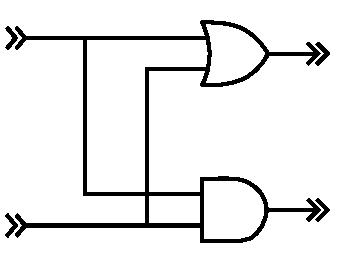
\includegraphics[width= 0.25 \textwidth]{Graphics/1bitCompare.pdf}
\caption{1-bit hardware \texttt{Compare-Exchange}}
\label{fig:bitcompare}
\end{figure}

Sometimes it might be necessary to employ a reverse \texttt{Compare-Exchange} operation, which will swap the elements such that they are in reverse sorted order. Such an operation is obviously just as viable and data-independent as the regular \texttt{Compare-Exchange} operation, but may sometimes give a larger degree of freedom in the description of algorithms.

\subsubsection{Deterministic Data-oblivious Sorting Algorithms}

Deterministic data-oblivious sorting algorithms form a large group of algorithms, though many of them are not known by their data-oblivious qualities, but instead as sorting networks.

\begin{figure}
\center
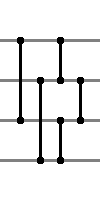
\includegraphics[width= 0.15 \textwidth]{Graphics/network.png}
\caption{4-wire sorting network, equivalent to \texttt{Compare-Exchange} for inputs $(0,2), (1,3), (0,1), (2,3), (1,2)$}
\label{fig:network}
\end{figure}

It is important to note that any fixed sorting network is a data-oblivious sorting algorithm, and can be modelled using \texttt{Compare-Exchange} operations, by performing such an operation for each comparison on the wires of the networks, as seen in Figure\ref{fig:network}. Additionally, any deterministic sorting algorithm depending entirely on \texttt{Compare-Exchange} operations can be viewed as a sorting network that runs a wire for each element of the input, and perform a comparison between wire contents wherever the algorithm performs a \texttt{Compare-Exchange} operation.

Due to their roots in sorting networks, data-oblivious sorting algorithms have a long history, and many algorithms have been developed to perform as sorting networks.

The historical algorithms of Bubble Sort~\citeB{BubbleSort} and the original Shellsort~\citeA{Shellsort} are both examples of simple algorithms that can easily be made data-oblivious by removing any checks for sortedness. This leaves them at their $\Theta(n^2)$ worst-case running time, but makes them easily understandable as data-oblivious algorithms.

Optimal sorting networks have been constructed, running in $\Theta(n \log n)$ time. The most famous of these networks is the AKS sorting network of~\citeA{AKS}, which is widely known, and form the basis of a great deal of research in the sorting networks field. Worth mentioning is also Zig-Zag Sort~\citeA{ZigZag} which is especially interesting due to its simplicity.
These optimal sorting networks are all entirely dependent on the usage of \textepsilon -halvers; a construction that is complicated to produce deterministically, and  has a very high constant factor to their number of comparison. The problem of constructing \textepsilon -halvers makes these optimal sorting networks of little use in practical implementations.

Pratt presents a more efficient variant of Shellsort in his thesis~\citeA{PrattThesis}, that is not only $\Theta(n \log^2 n)$ in the amount of comparisons, but also easily translates into a sorting network. The main idea of Pratt's variant Shellsort, is using a special $\Theta(\log^2 n)$-length jump sequence, instead of the old-fashioned geometric sequences that are often used in Shellsort.

A final interesting family of sorting networks are the algorithms stemming from Batcher's paper on sorting networks~\citeA{SNApplications}, known as Bitonic Sort and Odd-Even Mergesort, along with the Pairwise Sorting Network~\citeA{PairwiseSorting}. These sorting networks achieve sorting at $\Theta(n \log^2 n)$ comparisons, while maintaining a $\Theta(\log^2 n)$ depth, and are simple enough to be implemented on standard hardware, though their asymptotical complexity makes them somewhat lacking when compared to non-oblivious sorting algorithms.

\subsubsection{Randomized Data-Oblivious Sorting Algorithms}

Randomized data-oblivious sorting algorithms are a fairly new development, primarily introduced by \citeA{RandShellSort} and \citeA{AnnealingSort}, but an interesting one. Unfortunately, the list of algorithms performing data-oblivious sorting using a randomized sequence of \texttt{Compare-Exchange} is somewhat short. They are however useful due to the fact that they are simple in their method of operations.

From~\citeA{AnnealingSort} we get Spin-the-bottle Sort and Annealing Sort. The former of which is a $\Theta(n^2 \log n)$ data-oblivious sorting algorithm, of interest only in setting the stage for Annealing Sort, which will with very high probability, sort any given input obliviously in $\Theta(n \log n)$ time.
It is worth noting that the amount of comparisons performed by Annealing Sort has a high constant coefficient if the values given in~\citeA{AnnealingSort} are used, but this could easily be the result of overly pessimistic analysis, as is also the case of~\citeA{RandShellSort}.

A variant of Shellsort, called Shaker Sort is presented in~\citeA{ShakerSort}, and can be implemented as a $\Theta(n \log n)$ sorting network.
Shaker Sort's main deviance from Shellsort is replacing the subsequence sorting with so-called \emph{h-shakes}, which are linear-complexity applications of \texttt{Compare-Exchange} operations up and down the subsequence. Despite having certain bad input permutations, Shaker Sort shows great potential in sorting randomized input data.
By shuffling the input sequence to break up inputs that have been carefully constructed as adversary inputs, we can obtain a randomized variant of Shaker Sort, that  will show excellent performance characteristics, though this requires data-oblivious constructs beyond the \texttt{Compare-Exchange} operation, and will make the algorithm unsuitable for construction as a pure sorting network.

Finally, from~\citeA{RandShellSort} we get Randomized Shellsort, an algorithm that will sort with very high probability in $\Theta(n \log n)$ time by performing \texttt{Compare-Exchange} among random matching pairings taken from regions of the input in regions of sizes matching the subsequence jumps of the original Shellsort algorithm.

Sorting networks can be constructed from randomized data-oblivious algorithms by recording the sequence of operations the algorithm would perform, and constructing the corresponding network. This will lead to networks that use the same amount of comparator components as the amount of \texttt{Compare-Exchange} operations used in algorithm, but the network might not adapt well in terms of depth.

\subsubsection{Algorithms Tabular}

Since the previous subsection includes a great amount of different algorithms, we here present them in short tabular form, as a quick reference sheet.
The table in question is Table~\ref{BigAlgTable}.
\begin{table}[!h]
\begin{adjustwidth}{-.5in}{-.5in}
\centering
\begin{tabular}{|c c c c|}
\hline
Name & Source & Running Time & Keywords \\\hline
Bubble Sort & ~\citeB{BubbleSort} & $\Theta(n^2)$ & Simple \\
Shellsort & ~\citeA{Shellsort} & varies & Customizable, Well-researched \\
AKS Sorting Network & ~\citeA{AKS} & $\Theta(n \log n)$ & Optimal, Theoretical, Depth-optimal \\
Zig-Zag Sort & ~\citeA{ZigZag} & $\Theta(n \log n)$ & Optimal \\
Pratt's Shellsort & ~\citeA{PrattThesis} & $\Theta(n \log^2 n)$ & Shellsort-based\\
Bitonic Sort & ~\citeA{SNApplications} & $\Theta(n \log^2 n)$ & Well-known, Practical \\
Odd-Even Mergesort & ~\citeA{SNApplications} & $\Theta(n \log^2 n)$ & Merge Sort \\
Pairwise Sorting Network & ~\citeA{PairwiseSorting} &  \textcolor{red}{$\Theta(n \log^2 n)$} & Simple \\
Spin-the-bottle Sort & ~\citeA{AnnealingSort} & $\Theta(n^2 \log n)$ & Randomized, Unused \\
Annealing Sort & ~\citeA{AnnealingSort} & $\Theta(n \log n)$ & Randomized, Impractical \\
Shaker Sort & ~\citeA{ShakerSort} & $\Theta(n \log n)$ & Shellsort-Based, Possible~Randomization \\
Randomized Shellsort & ~\citeA{RandShellSort} & $\Theta(n \log n)$ & Randomized, Shellsort-based \\\hline
\end{tabular}
\end{adjustwidth}
\caption{Table of algorithms}
\label{BigAlgTable}
\end{table}

\subsection{Other Data-Oblivous Algorithms}

Most of the work done in the field of data-oblivious algorithms concerns itself with the sorting of numbers. This stems from the existence of sorting networks as an already established field, and the nature of sorting giving itself easily to the concept of data obliviousness. There are however other classes of data-oblivious algorithms, though they are scarce, and not always easily adaptable to modern hardware.

In order to construct a probabilistic sorting network probabilistic data-oblivious algorithms for merging and selection are presented in~\citeB{ProbNetworks}. Data-oblivious merging is already made possible by~\citeA{SNApplications} in $\Theta(n \log n)$ time, and this running time is not asymptotically improved, but the paper shows that the problem of data-oblivious selection is faster than any known solution to data-oblivious sorting.

Selection, along with compaction and sorting, is also explored in~\citeB{ObliviousExternal} using the external memory model, as a means to provide a solution for such problems, when one must perform privacy-preserving computations on externally located data. Note that for data-oblivious algorithms in the external memory model, any computations are allowed in internal memory, and only the accesses to external memory needs to be kept oblivious.

A great number of set operations are shown to be computable in an oblivious and privacy-preserving manner in~\citeB{ObliviousSet}. These algorithms can become the fundamental building blocks for later algorithms, and are therefore of great significance to the field of data-oblivious algorithms.

Several crucial graph algorithms, namely breath-first search, single-source shortest distance, maximum flow and minimum spanning tree, have efficient data-oblivious algorithms for dense graphs presented in~\citeB{ObliviousGraph}. These are especially interesting, as they venture far from the well-known area of sorting, and can be useful for doing multi-party network routing computations, where one might wish to keep the algorithm oblivious due to privacy concerns.

A number of geometric problems, convex hull, quadtree construction, closest pair and all-nearest-neighbours have data-oblivious solutions presented in~\citeB{GraphGeoOblivious}. These serve as useful building blocks for applications that are privacy-preserving, distributed and location-aware. 

Finally, it should be noted that the existence of the concept \emph{Oblivious RAM} is often mentioned in the data-oblivious literature. Oblivious RAM is an ingenious concept originating from~\citeB{ObliviousRam} that allows the execution of arbitrary algorithms in a manner that prevents an adversary from obtaining useful information about the input from the memory accesses of the algorithm. This is especially useful for privacy-preserving computations, but imposes a non-constant overhead on the complexity of the program, which means that the development of optimal data-oblivious algorithms is still relevant.
\label{ch:intro}

%%%%%%%%%%%%%%%%%%%%%%%%%%%%%%%%%%%%%%%%%%%%%%%%%%%%%%%%%%%%%%%%%%%%%%%

\chapter{Data-Oblivious Sorting Algorithms}
\label{ch:algorithms}

Throughout this thesis, several data-oblivious sorting algorithms will be discussed, and their properties relating to efficiency and optimization techniques will be studied. Before we can continue on to this work, we must however ensure that we have established the structure of these algorithms, and most of this chapter will devote itself to brief descriptions of the individual algorithms that form the basis of any further work being done.

Let us begin by immediately describing these algorithms. 

\section{Randomized Shellsort}

Randomized Shellsort~\citeA{RandShellSort} is a randomized data-oblivious sorting algorithm notable for its ability to sort data with very high probability, using only $\Theta(n \log n)$ comparisons.

The algorithm itself is fairly simplistic, consisting entirely of applications of a special region comparison function, whose method of operation will be described shortly. This can then optionally be followed by clean-up phase entirely constructed from already known data-oblivious sorting algorithms.

It is especially important to note that the size and location of regions being compared will be entirely dependent on the size of the data, and that matchings between elements is determined randomly with no knowledge of the input.

The analysis showing the low failure rate of the algorithm is unfortunately rather lengthy, and somewhat complex, but can be found in~\citeA{RandShellSort}.

\subsection{Region Comparison}
\label{sec:RegionCompare}

The comparison between regions is done by computing a random matching between elements of the two regions, and performing a \texttt{Compare-Exchange} operation between each pair of matched indices.
This procedure will be repeated $c$ times to perform a full comparison of regions.~\citeA{RandShellSort} shows that when $c \geq 4$ the full region comparison will have properties closely related to those of \textepsilon -halvers.

The pseudo-code for the region comparison is shown in Algorithm~\ref{RegionCompare}.

For a graphical representation of the region comparison, see Figure~\ref{fig:CompareExchange}.


\begin{algorithm}
\caption{Region Compare}\label{RegionCompare}
\begin{algorithmic}[1]
	\Statex $A$: Array input of \texttt{Compare-Exchange} compatible elements
	\Statex $i$: Index of first region
	\Statex $j$: Index of second region
	\Statex $size$: Size of regions to compare
\Procedure{RegionCompare}{$A, i, j, size$}
\For{$1 \dots c$}
	\Comment $c$ is a predetermined constant
	\State $matching \gets \mathtt{shuffle}([0 \dots size-1])$
	\For{$k = 0 \dots size-1$}
		\State $\mathtt{Compare\mbox{-}Exchange}(A, i + k, j + matching[k])$
	\EndFor
\EndFor
\EndProcedure
\end{algorithmic}
\end{algorithm}

\begin{figure}
\center
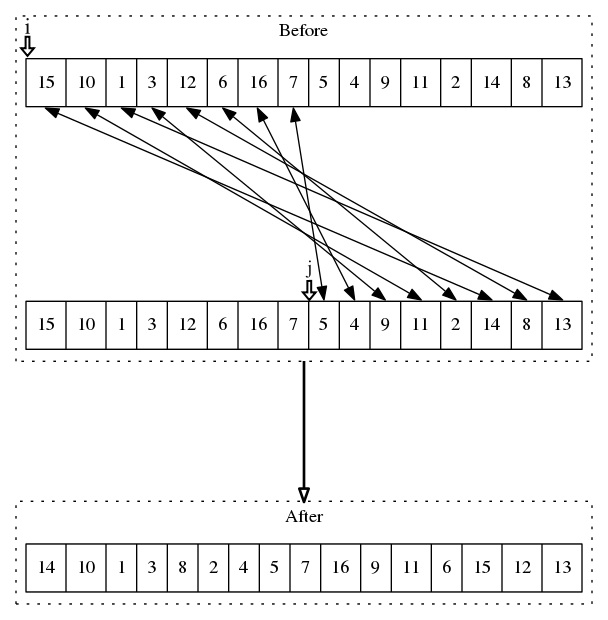
\includegraphics[width=\textwidth]{Graphics/regcmp.png}
\caption{Region Compare with $c=1$ of size 8 on 16 elements of data. $i$ and $j$ are the first and last halves of the shown arrays respectively. Note that the \emph{Before} region shows the matching with the same array.}
\label{fig:CompareExchange}
\end{figure}

\subsection{The Main Algorithm}

Having constructed the region comparison operation, we move on to the main algorithm.

The important part of Randomized Shellsort consist of applying the region comparison on the input data in ever decreasing region sizes, starting at $n/2$, and halving in size until they reach $1$. Note that there will be only $\log(n)$ such region sizes, and that $n$ is assumed to be a non-trivial power of 2.

For each region size, six different runs through the data are performed. These runs fall into two distinct groups, a \emph{shaker} phase and a \emph{brick} phase.

In the \emph{shaker} phase we run through the regions, comparing them with the next region in ascending order, and then do the same for descending order. This resembles the variant of Shellsort called Shaker Sort~\citeA{ShakerSort}, and is intended to quickly move misplaced elements to the correct end of the input.

The \emph{brick} phase will first run through the regions comparing them to the regions $3$ places further up, then a run comparing $2$ places up, and then finally it will perform runs comparing first the even regions with their next neighbour, and then the odd regions with their next neighbour.
This somewhat resembles the Brick Sort mentioned in~\citeB{ShellsortRelated}, and it is important for the analysis that this sequence of comparisons creates a complete 4-tournament of any 4 adjacent regions.
This phase serves the purpose of moving elements short distances among nearby regions of the input. 

Finally, following the main part of the algorithm, a clean-up step is taken to move a polylogarithmic amount of stray elements into place.~\citeA{RandShellSort} notes that this can be done by repeated applications of Pratt's variant of Shellsort~\citeA{PrattThesis}, but states that this final clean-up step is most likely needed only as an artefact from the analysis of the sorting probability.

It is fairly easy to see that if we can perform the region comparison in linear time, then the main algorithm will perform $\Theta(n \log n)$ operations. Using the region comparison of Section~\ref{sec:RegionCompare}, we can easily guarantee linear time region comparisons, leading to the desired running time. 

Given this sequence of region comparisons, and the \texttt{RegionCompare} procedure from Algorith~\ref{RegionCompare}, it is clearly seen that the Randomized Shellsort will perform at most $5cn\log n$ comparisons in addition to the clean-up phase, which is low compared to the huge constants of~\citeA{AKS}, if $c$ is kept at a reasonable level.

The exact structure of the algorithm is best described in pseudo-code, as seen in Algorithm~\ref{RandomizedShellsort}.

\begin{algorithm}
\caption{Randomized Shellsort}\label{RandomizedShellsort}
\begin{algorithmic}[1]
	\Statex $A$: Array input of \texttt{Compare-Exchange} compatible elements
	\Statex $n$: Size of $A$
\Procedure{RandomizedShellsort}{$A, n$}
\For{$jump = n/2, n/4, n/8 \dots 1$}
	\For{$i = 0 \dots n/jump-2$}
	\Comment Shaker pass part 1
		\State $\mathtt{RegionCompare}(A, i\cdot jump, (i+1)\cdot jump, jump)$
	\EndFor
	\For{$i = n/jump-1 \dots 1$}
	\Comment Shaker pass part 2
		\State $\mathtt{RegionCompare}(A, (i-1)\cdot jump, i\cdot jump, jump)$
	\EndFor
	\For{$i = 0 \dots n/jump-4$}
	\Comment Brick pass part 1
		\State $\mathtt{RegionCompare}(A, i\cdot jump, (i+3)\cdot jump, jump)$
	\EndFor
	\For{$i = 0 \dots n/jump-3$}
	\Comment Brick pass part 2
		\State $\mathtt{RegionCompare}(A, i\cdot jump, (i+2)\cdot jump, jump)$
	\EndFor
	\For{$i = 0, 2, 4 \dots n/jump-2$}
	\Comment Brick pass part 3
		\State $\mathtt{RegionCompare}(A, i\cdot jump, (i+1)\cdot jump, jump)$
	\EndFor
	\For{$i = 1, 3, 5 \dots n/jump-3$}
	\Comment Brick pass part 4
		\State $\mathtt{RegionCompare}(A, i \cdot jump, (i+1)\cdot jump, jump)$
	\EndFor
\EndFor
\State $\mathtt{Clean-Up(A)}$
\EndProcedure
\end{algorithmic}
\end{algorithm}


\FloatBarrier 
\section{Annealing Sort}

Annealing Sort~\citeA{AnnealingSort}, like Randomized Shellsort, is a randomized data-oblivious sorting algorithm that will sort data with very high probability in $\Theta(n \log n)$ \texttt{Compare-Exchange} operations.

Annealing Sort borrows its name from Simulated Annealing~\citeB{SimulatedAnnealing}, the algorithmic paradigm that inspired the algorithm, but since sorting is not an optimization problem, the basic pattern of Simulated Annealing is only slightly related to the actual operations of the algorithm.

When considering this algorithm, keep in mind that the algorithm performs a random pattern of \texttt{Compare-Exchange} operations based entirely on the size of the input, which qualifies it as a randomized data-oblivious algorithm.

\subsection{The Main Algorithm}
\label{sec:AnnealingSortMain}

Annealing Sort relies on a sequence of temperatures and repetitions, referred to as the \emph{annealing schedule}. This schedule is entirely dependent on input size, and picking a good sequence for this schedule is crucial to both the performance and correctness of the algorithm.

For each entry in the annealing schedule, consisting of a temperature $t$ and a repetition count $r$, the algorithm will perform a run through the input data, performing $r$ \texttt{Compare-Exchange} operations between the current index, and elements at most $t$ further up the input. 
This is followed by a similar run, going backwards, comparing elements to those further down the input.

In loose terms, this is similar to the \emph{shaker} phases of Randomized Shellsort, and the analysis of the algorithm closely follows that of~\citeA{RandShellSort}, but instead of having fixed borders betweens regions, they slide up and down the input following the current element.

Note that the algorithm will perform at most $2n\cdot\sum{r_i}$  \texttt{Compare-Exchange} operations, where $r_i$ specifies the number of repetitions in the entry $i$ of the annealing sequence.

The algorithm in described using pseudo-code in Algortihm~\ref{AnnealingSort}.
If nothing else, the algorithm is beautifully simple, once the annealing sequence is known.

\begin{algorithm}
\caption{Annealing Sort}\label{AnnealingSort}
\begin{algorithmic}[1]
	\Statex $A$: Array input of \texttt{Compare-Exchange} compatible elements
	\Statex $n$: Size of $A$
\Procedure{AnnealingSort}{$A, n$}
\For {$(t, r)$ in Annealing Sequence}
	\For {$i = 0 \dots n-2$}
		\For{$j = 1 \dots r$}
			\State {$\mathtt{Compare\mbox{-}Exchange}(A, i, \mathtt{random\mbox{-}choice}([i+1: \min(i+t, n-1)]))$}
		\EndFor
	\EndFor
	\For {$i = n-1 \dots 1$}
		\For{$j = 1 \dots r$}
			\State {$\mathtt{Compare\mbox{-}Exchange}(A, \mathtt{random\mbox{-}choice}([\max(i-t, 0): i-1]), i)$}
		\EndFor
	\EndFor
\EndFor
\EndProcedure
\end{algorithmic}
\end{algorithm}


\subsection{Annealing Schedule}

As mentioned in Section~\ref{sec:AnnealingSortMain}, finding the right Annealing Schedule plays a big role in Annealing Sort. Luckily~\citeA{AnnealingSort} shows how to construct a 3-part schedule that will both keep the number of \texttt{Compare-Exchange} operations at $\Theta(n \log n)$, and make the algorithm sort with very high probability.

The annealing schedule is as follows;

\begin{description}
\item[Phase one:] $[(n/2, c), (n/2, c), (n/4, c), (n/4, c) \dots (q \log^6 n, c), (q \log^6 n, c)]$ for some $q \geq 1$ and $c > 1$
\item[Phase two:] $[(q \log^6 n, r),((q/2) \log^6 n, r), ((q/4) \log^6 n, r) \dots (g \log n, r)]$ using $q$ from phase one, $g \geq 1$,  and $r$ being $\Theta(\frac{\log n}{\log \log n})$
\item[Phase three:] $[(1,1), (1,1) \dots (1,1)]$ of length $g \log n$
\end{description}

Concatenating these three sequences, we get the desired annealing schedule.

In the analysis, it is hinted that we want $c \geq 9$ and $g = 64e^2$, but little effort is done in determining $q$ and a suitable factor for $r$. Though these constant factors seem impractically large, they may easily be the result of an overly pessimistic analysis, and an experimental evaluation of the proper scale of these factors is presented in Section~\ref{sec:AnnealingExperiments}.

When using this annealing schedule, the total number of \texttt{Compare-Exchange} operations per $n$ will be 
\[
2c \max(0, \log 2n - \log (q \log^6 n)) + r \max(0,\log (q \log^6 n) - \log (g \log n)) + g \log n
\]

Since we have $c$, $q$, $g$ all constants bigger than 0, and $r=\Theta(\frac{\log n}{\log \log n})$ this gives us:

\begin{multline*}
2c \max(0, \log 2n - \log (q \log^6 n)) + r \max(0,\log (q \log^6 n) - \log (g \log n)) + g \log n
\\
\le 2c \log 2n  + r \log (q \log^6 n) + g \log n
=
\Theta(\log n)\\
\end{multline*}

This gives the algorithm a total running time of $\Theta(n \log n)$.


\FloatBarrier
\section{Bitonic Sort} 
\label{sec:BitonicSort}

Bitonic Sort is one of the earliest sorting networks, and was presented in~\citeA{SNApplications}. The algorithm is based on the concept of bitonic sequences, which is a sequence constructed as the juxtaposition of an ascending and a descending sequence, and the operation of the algorithm is based on constructing and merging bitonic sequences.

The algorithm suffers from a running time of $\Theta(n \log^2 n)$, but it works well in practice due to having small constants, and being suitable for compile-time optimisation.

\subsection{Bitonic Merging}

The one basic idea behind Bitonic Sort, is that any bitonic sequence can be sorted with relative ease by a sorting network.

The main part of this sorting consist of a bitonic split\footnote{
The \emph{bitonic split} is also referred to as the \emph{bitonic merge} in most of this thesis, despite not actually merging sequences. The \emph{merge} misnomer originates in the structure of the algorithm, where the \emph{bitonic split} takes the role of a merge in a classic mergesort. The \emph{bitonic merge} merge may also be seen as merging an ascending and a descending sequence into a single sorted sequence.
}, which given a bitonic sequence $A$ of length $N$ creates

\begin{equation}
\begin{split}
&HI = \{\max(a_1, a_{n/2+1}), \max(a_2, a_{n/2+2}), \max(a_3, a_{n/2+3}) \dots \max(a_{n/2}, a_n)\}\\
\\
&LO = \{\min(a_1, a_{n/2+1}), \min(a_2, a_{n/2+2}), \min(a_3, a_{n/2+3}) \dots \min(a_{n/2}, a_n)\}
\end{split}
\end{equation}

\noindent
where $HI$ and $LO$ are bitonic sequences of length $N/2$, and any element in $HI$ is bigger than all elements $LO$. These properties of $HI$ and $LO$ are determined in~\citeA{SNApplications}. 

Since the bitonic split moves the elements to a low and a high half, and both halves are still bitonic sequences, we can sort a bitonic sequence by recursively applying bitonic split. The recursive operation is described in Algorithm~\ref{BitonicMerge}

\begin{algorithm}
\caption{Bitonic Merge}\label{BitonicMerge}
\begin{algorithmic}[1]
	\Statex $A$: Bitonic array input of \texttt{Compare-Exchange} compatible elements
	\Statex $n$: Size of $A$
\Procedure{BitonicMerge}{$A, n$}
\If {$n>1$}
	\For {$i = 0 \dots n/2-1$}
		\State {$\mathtt{Compare\mbox{-}Exchange}(A, i, i+n/2)$}
	\EndFor
	\State{$\mathtt{BitonicMerge}(A[0 \dots n/2-1], n/2)$}
	\State{$\mathtt{BitonicMerge}(A[n/2 \dots n-1], n/2)$}
\EndIf
\EndProcedure
\end{algorithmic}
\end{algorithm}

\subsection{The Main Algorithm}

Given the bitonic merge operation, we can construct a sorting algorithm by exploiting the fact that the concatenation of an ascending and a descending sequence will be a bitonic sequence.

\begin{thm}
If we can sort bitonic sequences, then we can sort any sequence of length $2^k$
\end{thm}

\begin{proof}
Simple induction proof:

\textbf{Base case - $2^0$:} Any sequence of length $2^0 = 1$ is already sorted.

\textbf{Inductive case - $2^k$:} Let $A$ be the first $2^{k-1}$ elements, and $B$ the last $2^{k-1}$ elements. Sort $A$ and $B$, reverse $A$, let $C = A+B$. $C$ is now a bitonic sequence containing the original elements, and since we can sort bitonic sequences using Algorithm \ref{BitonicMerge}, we can sort the original elements.
\end{proof}


This gives us a fairly simple way of sorting using the bitonic merging procedure, as shown in Algorithm~\ref{BitonicSort}.

\begin{algorithm}
\caption{Bitonic Sort}\label{BitonicSort}
\begin{algorithmic}[1]
	\Statex $A$: Array input of \texttt{Compare-Exchange} compatible elements
	\Statex $n$: Size of $A$
\Procedure{BitonicSort}{$A, n$}
\If {$n>1$}
	\State{$\mathtt{BitonicSort}(A[0 \dots n/2-1], n/2)$}
	\State{$\mathtt{BitonicSort}(A[n/2 \dots n-1], n/2)$}
	\State{$\mathtt{Reverse}(A[0 \dots n/2-1])$}
	\State{$\mathtt{BitonicMerge}(A, n)$}
\EndIf
\EndProcedure
\end{algorithmic}
\end{algorithm}

The $\Theta(n \log^2 n)$ total amount of \texttt{Compare-Exchange} operations performed by the algorithm follows from the Master Theorem \textcolor{red}{and exercise 4.6-2} of~\citeB{Cormen}.






\FloatBarrier
\section{Odd-Even Mergesort} 
\label{sec:OddEvenMergesort}

Odd-Even Mergesort is the sister algorithm of Bitonic Sort, and also comes from~\citeA{SNApplications}. The idea of requiring bitonic sequences for merging in  Bitonic Sort seems unintuitive, and Odd-Even Mergesort does away with that requirement, at the expense of slightly more complicated merging operation.
Like Bitonic Sort, Odd-Even Mergesort performs $\Theta(n \log^2 n)$ comparisons, but the constant factors involved are slightly lower.

\subsection{Odd-Even Merging}

Given two sorted sequences, it is possible to merge them by dividing them into their odd and even parts, and then combining them into an interleaved sequence.

The intuition of this merging scheme follows from the following observation:

\noindent
Let $A$ and $B$ be sorted sequences of length $N$.

\noindent
Let $C$ be the sorted merge of $A$ and $B$.

$C$ might look something like this:

\[
C = {a_0, b_0, b_1, b_2, a_1, a_2, b_3 \dots}
\]

or

\[
C = {b_0, b_1, a_0, b_2, a_1, b_3, b_4 \dots}
\]

Now, imagine a grouping of $C$ as follows; 

\[
C = {a_0,(b_0, b_1), (b_2, a_1), (a_2, b_3) \dots}
\]

or

\[
C = {b_0, (b_1, a_0), (b_2, a_1), (b_3, b_4) \dots}
\]

What we see here, is that every pair of parenthesized numbers is made up of one odd-indexed number and one even-indexed. In fact~\citeA{SNApplications} shows that every merged sequence of two sorted sequences will follow this rule, and we can use this to construct $C$ in the following way.

Divide $A$ and $B$ into odd and even indexes, and merge them recursively. Pick $c_0 = even_0$, pick $c_1 = \min(odd_0, even_1)$, $c_2 = \max(odd_0, even_1)$, $c_3 = \min(odd_1, even_2)$, $c_4 = \max(odd_1, even_2)$ \dots and so on. In case there is only one element in each subsequence, just perform a single \texttt{Compare-Exchange}. This gives us the following algorithm, shown as pseudo-code in Algorithm~\ref{OddEvenMerge}.

\begin{algorithm}
\caption{Odd-Even Merge}\label{OddEvenMerge}
\begin{algorithmic}[1]
	\Statex $A$: Array input of \texttt{Compare-Exchange} compatible elements
	\Statex $B$: Array input of \texttt{Compare-Exchange} compatible elements
	\Statex $n$: Size of $A$ and $B$
\Procedure{OddEvenMerge}{$A, B, n$}
\If {$n=1$}
	\State $C \gets [{A[0], B[0]}]$
	\State $\mathtt{Compare-Exchange}(C, 0, 1)$
\Else
	\State {$odd \gets \mathtt{OddEvenMerge}(\mathtt{odd}(A),\mathtt{odd}(B), n/2)$}
	\State {$even \gets \mathtt{OddEvenMerge}(\mathtt{even}(A),\mathtt{even}(B), n/2)$}
	\For {$i = 0 \dots n/2-1} $
		\State {$C[2i] \gets even[i]$}
		\State {$C[2i+1] \gets odd[i]$}
	\EndFor
	\For {$i = 0 \dots n/2-2} $
		\State {$\mathtt{Compare\mbox{-}Exchange}(C, 2i+1, 2i+2)$}
	\EndFor
\EndIf
\EndProcedure
\end{algorithmic}
\end{algorithm}

\subsection{The Main Algorithm}

Given the Odd-Even merge construction, we can perform a straight-forward merge sort.

The interesting part of Odd-Even Mergesort is perhaps that it is possible to construct a merging network that has so few prerequisites, which leads to an exceptionally simple algorithm. Unfortunately, the price of having a simple merge sort, is a more complex merge step.

The exact procedure for merge sorting using Odd-Even Merging is shown as pseudo-code in Algorithm~\ref{OddEvenMergeSort}

\begin{algorithm}
\caption{Odd-Even Mergesort}\label{OddEvenMergeSort}
\begin{algorithmic}[1]
	\Statex $A$: Array input of \texttt{Compare-Exchange} compatible elements
	\Statex $n$: Size of $A$
\Procedure{OddEvenMergeSort}{$A, n$}
\If {$n>1$}
	\State{$\mathtt{OddEvenMergeSort}(A[0 \dots n/2-1], n/2)$}
	\State{$\mathtt{OddEvenMergeSort}(A[n/2 \dots n-1], n/2)$}
	\State{$\mathtt{OddEvenMerge}(A[0 \dots n/2-1], A[n/2 \dots n-1], n)$}
\EndIf
\EndProcedure
\end{algorithmic}
\end{algorithm}

The running time of Odd-Even Mergesort, like Bitonic Sort follows from the Master Theorem  \textcolor{red}{and exercise 4.6-2} of~\citeB{Cormen}.


\FloatBarrier
\section{Shellsort Variants} 

Shellsort, as described by~\citeA{Shellsort}, has been around for a long time, and a great deal of research has been dedicated to studying its performance. Shellsort works by sorting subsequences consisting of every $k$'th element using Insertion Sort, for given values of $k$\footnote{
The original Shellsort uses $n/2, n/4, n/8 \dots 1$, but many different sequences of $k$ can be used.
}.  As a sorting network, we can replace the internal Insertion Sort with Bubble Sort to construct an $\Theta(n^2)$ data-oblivious sorting algorithm, though doing so is thoroughly unimpressive, as the final step consists of simply running Bubble Sort on the entire input.

There are however data-oblivious variants of Shellsort that perform well, both in theory and practice, and no study of data-oblivious algorithms would be complete without including at least a few of them.

\subsection{Pratt's Shellsort}

Pratt's PhD thesis~\citeA{PrattThesis} not only shows that the most common variants of Shellsort must use $\Omega(n^{3/2})$ comparisons in the worst case, but also manages to produce a special sequence for Shellsort most commonly known as the Pratt Sequence.

The Pratt sequence for Shellsort consists of all the numbers on the form $2^i3^j < n$, in a specially constructed order. This sequence has length $\Theta(\log^2n)$, which in itself is long for a Shellsort sequence, but has a desirable property of bounding the complexity of the internal subsequence sorting to a linear amount of comparisons, which can be used to produce an $\Theta(n \log^2 n)$ data-oblivious algorithm.

When adapting the Pratt sequence and the reduced inner sort directly, we can construct a simple algorithm that constructs the sequence, and performs the necessary comparisons at the same time, as described in the pseudo-code of Algorithm~\ref{alg:Pratt}.

\begin{algorithm}
\caption{Pratt's Shellsort}\label{alg:Pratt}
\begin{algorithmic}[1]
	\Statex $A$: Array input of \texttt{Compare-Exchange} compatible elements
	\Statex $n$: Size of $A$
\Procedure{PrattSort}{$A, n$}
\For {$i = n/2, n/4, n/8 \dots 1$}
	\State{$j \gets i$}
	\Do
		\For {$k = 0 \dots n-j-1$}
			\State {$\mathtt{Compare-Exchange}(A,k,k+j)$}
		\EndFor
		\State {$ j \gets 3j/2$}
	\doWhile {$j \% 3 == 0\ \text{and}\ j < n$}
\EndFor
\EndProcedure
\end{algorithmic}
\end{algorithm}

\subsection{Shaker Sort}

Shaker Sort\footnote{
A certain Bubble Sort variant also goes by the name of (Cocktail) Shaker Short. Any reference to Shaker Sort in this thesis is to the Shellsort variant of~\citeA{ShakerSort}.
}, as described in~\citeA{ShakerSort} is another interesting variation of Shellsort. Shaker Sort replaces the subsequence sorting with a single upwards and downwards \texttt{Compare-Exchange} scan, called a Shaker Pass. There appears to be little analytical work done in determining the failure rate of Shaker Sort, but it is known that certain sequences of length $\Theta(\log n)$ seem effective at sorting random data.

The algorithm can be described as seen in Algorithm~\ref{alg:ShakerSort}.


It should be noted, that~\citeA{BadShaker} shows that certain input sequences will make Shaker Sort fail unless the amount of 1-shakes is linear in the size of the input. These sequences do not appear to be stable under shuffling, which could solve this problem, and it is also noted that for sorting random input, Shaker Sort still seems to have a negligible failure rate.

\begin{algorithm}
\caption{Shaker Sort}\label{alg:ShakerSort}
\begin{algorithmic}[1]
	\Statex $A$: Array input of \texttt{Compare-Exchange} compatible elements
	\Statex $n$: Size of $A$
\Procedure{ShakerSort}{$A, n$}
\State {$\mathtt{Shuffle}(A)$} 
\Comment{Shuffle is optional, but advised for general inputs.}
\State {$seq \gets \mathtt{ShakerSequence}(n)$}
\ForAll {$s\ \mathbf{in}\ seq$}
	\For {$i = 0 \dots n-s-1$}
		\State {$\mathtt{Compare-Exchange}(A,i, i+s)$}
	\EndFor
	\For {$i = n-1 \dots s$}
		\State {$\mathtt{Compare-Exchange}(A,i-s, i)$}
	\EndFor
\EndFor
\EndProcedure
\end{algorithmic}
\end{algorithm}





\FloatBarrier
\section{Algorithms Recap} 

\begin{table}[!h]
\begin{tabular}{|c c c c|}
\hline
Name & Running Time &  Failure Rate & Parallelism \\ \hline
Randomized Shellsort & $\Theta(n \log n)$ & $1/n^b, b \geq 1$ & Some \\

Annealing Sort & $\Theta(n \log n)$ & $1/n^b, b \geq 1$ & Minor \\

Bitonic Sort & $\Theta(n \log^2 n)$ & 0 & Highest \\

Odd-Even Mergesort & $\Theta(n \log^2 n)$ & 0 & High/Highest \\

Pratt's Shellsort & $\Theta(n \log^2 n)$ & 0 & High \\

Shaker Sort & $\Theta(n \log n)$ & ? \tablefootnote{Failure rate is dependent on input permutations, and mostly verified experimentally, but low in practice with random input data.} & High\\
\hline
\end{tabular}
\caption{Overview of used algorithms}
\label{AlgTable}
\end{table}

Due to the high number of algorithms present in this thesis, we provide a table listing the different algorithms used in the experiments, and their properties. 

One thing that is painfully obvious from Table~\ref{AlgTable} is the lack of an $O(n \log n)$ algorithm with 0 failure rate. Such algorithms do exist, as explained in the introduction of this thesis, but are both impractical to implement, and have horrible constant factors involved in their running times.



\FloatBarrier
\section{Survey of Additional Algorithms}

Despite the great number of algorithms presented in the previous sections of this chapter, there are still many data-oblivious sorting algorithms that have not yet been described.
The reason these algorithms have been omitted until now, is their exclusion from the already crowded experiments and implementation chapters.
In short, there are already too many algorithms to keep track of, and some algorithms simply aren't suited for the real world.

Many of these algorithms are still interesting from a theoretical point of view, but often fail to present a proper case for real-world usage.
Since these algorithms are still interesting for a general understanding of the field of sorting networks, this section will provide a short survey on the work that has been done in their design and analysis.

\subsection{The AKS sorting network}

The AKS sorting network of~\citeA{AKS} is perhaps one of the most famous sorting networks ever presented. 
This network remarks itself by being the first sorting network that is asymptotically optimal in the amount of comparisons and depth, but also has reputation for having enormous constant factors and being horrendously difficult to implement.

The basic construction of the AKS sorting network relies on partitioning the input into halves, quarters, eights and so forth, arranging these partitions as a binary tree, and applying a constant-depth network called an \textepsilon -nearsorter on the triplets formed by a node and its children. This is done for even and odd nodes one after another, a logarithmic number of times, giving the logarithmic depth to the network. As these operations proceed, the indices that any node is responsible for filter down through the tree, until finally all elements have arrived at 1-element leaf. A much more thorough description is given by~\citeA{AKS}, but little time is devoted to the practicalities of any actual construction of the network, as the authors wish to focus primarily on theory.

As the interest in optimal sorting networks continues, we see refinements of the AKS sorting network emerge. One of the most well-known of these is the sorting network of~\citeB{Paterson}, known of just as the Paterson sorting network. The Paterson sorting network follows many of the same ideas as the AKS sorting network, but replaces the \textepsilon -nearsorters with \textepsilon -separators, a structure that requires fewer comparisons by focusing more explicitly on moving extreme elements to the ends of the input. The new structure also simplifies the description of the destination for wires throughout the network, bringing it closer to an implementable construction. Given the more rigorous description of the network,~\citeB{Paterson} manages to calculate the amount of comparison performed, and place the depth of the network at about $6100 \log n$.

A variation of the Paterson sorting network is further explored in~\citeB{SNSimplified}, leading to a simple description of the network using a slightly less precise description of separators. Unfortunately the paper does not go into detail in attempting to keep the constant factors of the network small, and the constant factors of the depth of the network does not seem to be as firmly defined as those of the Paterson network..

Further improvements of the AKS sorting network are presented in~\citeB{AKSLectureNotes}, where the tree structure of the AKS sorting network is expanded to support a much larger branching factor, and useful multi-way separators are constructed from smaller sorting networks of fixed size. 
This result puts the depth of the network at $1830 \log n - 58657$, requiring $n \geq 2^{78}$. This depth is impressive in the world of optimal sorting networks, but unfortunately still not competitive with simpler networks for any reasonable $n$.

The networks based on AKS are all fairly similar, and have few competitors. There is however at least one other sorting network providing optimal size, though not depth. This new network, called Zig-zag Sort is presented in~\citeA{ZigZag}, and shows a new approach to optimal sorting networks, as it focuses more on size and simplicity than depth. Accepting a deep network with fewer comparisons allows for a network that is easy to construct, and has a much better constant factor in practice. A big part of the improvement in the amount of comparisons comes from using \textepsilon -halvers with a much lower precision than those of the previous networks, as the size and depth of such networks grows quickly as one requires higher precision.

This concludes the observations made on the AKS sorting network and its variants, and we now move on to less efficient networks.

\subsection{The $\Theta(n \log^2 n)$ Sorting Networks}

Numerous ingenious sorting networks have been developed throughout research history, many of them achieving a $\Theta(n \log^2 n)$ bound on their number of comparisons, but due to a lack of space, only a few of them have been included in this thesis.
While Bitonic Sort, Odd-Even Mergesort and Pratt's Shellsort are included in the experiment for their historical significance, practical performance and structural simplicity, they are far from the only networks to achieve some, or all, of these properties, and in this section a few other contenders will be discussed.

The Pairwise sorting network, described in~\citeA{PairwiseSorting}, remarks itself by being exactly the same size and depth as the Odd-Even Mergesort network. This may not seem impressive at first, but at the time of publication, it was claimed to be the first network to achieve this size in 20 years. The network is fairly simple, and starts by partitioning the input into sorted pairs, lexicographically sorting these pairs by recursion, and then merging the pairs into sorted order. The description of the network relies heavily on the \emph{0-1 principle} of~\citeB{Knuth3}, but is otherwise exceptionally simple, and the resulting sorting network is easily constructed in practice.

As mentioned, there has not been many successful attempts at constructing a deterministic sorting network having a lower complexity than Odd-Even Mergesort, while still being constructable in practice, though it is actually possible. An interesting generalisation of the Odd-Even Mergesort network is shown in~\citeA{DivideSortMerge}, which can reduce the number of comparisons performed by a $\Theta(n log n)$ amount, though this is only a minor gain since the algorithm retains the same constant factor for for it's $n log^2 n$ term. What is most notable about the generalized network presented in~\citeA{DivideSortMerge} is the construction of merging networks for more than two input streams, leading to a multi-way merge sort, which distinguished the network from its competitors. 

The Periodic Balanced Sorting Network of~\citeA{PeriodicSortingNetwork} utilizes a single block of $\Theta(\log n)$ depth to achieve sorting in $\Theta(n \log^2 n)$ time by $\log n$ applications of the aforementioned block. Using this construction they create a sorting network that, if constructed by exact duplicates of the same block, has a higher constant factor than competing networks. By skipping certain phases of the basic building block of the network the size of the network is brought close to that of Bitonic Sort. The repeatable nature of Periodic Sort is what makes it interesting, since it allows for an efficient hardware implementation, where data is repeatedly cycled through a single hardware component, and additionally allows for faulty comparators by increasing the amount of cycles.

Finally, if the base element of the sorting network is not the standard network comparators, but instead small $k$-sorters,~\citeA{kSorters} shows how to construct an $\Theta(n \log^2 n)$ sorting network. The algorithm presented in the paper is a slight variation of Columnsort from~\citeB{ColumnSort} to recursively construct merging network from $k$-sorters, which is utilizing in sorting the entirety of the input data.



%%%%%%%%%%%%%%%%%%%%%%%%%%%%%%%%%%%%%%%%%%%%%%%%%%%%%%%%%%%%%%%%%%%%%%%

\chapter{Implementing Data-Oblivious Sorting Algorithms}
\label{ch:Implementations}

Having given high-level descriptions of the major algorithms involved in this thesis, let us look at the practicalities of implementing such algorithms.

Special consideration should be given to the optimization techniques used for general performance increases across several algorithms, though many of the algorithms have individual peculiarities that are important for efficient implementations.

\section{Algorithm-Specific Implementation Notes} \FloatBarrier
\label{sec:specificimpl}

\subsection{Randomized Shellsort}

The analysis for Randomized Shellsort given in~\citeA{RandShellSort} requires $c \geq 4$, and a clean-up phase to remove a small amount of straggling elements.
It is however mentioned in the paper, that both the clean-up phase, and the high value of the constant $c$ are the results of an overly pessimistic analysis, and they show that the algorithm will sort with very high probability using $c = 1$ and no clean-up phase. Our own testing suggests the same, and the Randomized Shellsort algorithm used in the tests has no clean-up, and a $c$ kept at 1.

Extending the algorithm to arbitrary $n$ consist of picking jump sizes that are of the form $2^k$ and smaller than $n$. This makes the last region extend beyond the input size if it is not also a power of 2, but this is easily negated by adjusting the loop condition of \texttt{RegionCompare} procedure of Algorithm~\ref{RegionCompare}. 
The description of the algorithm assumes that $n$ is a power of 2, and that region sizes can be obtained by repeatedly halving the size. If $n$ is not a power of two, and one blindly constructs region sizes by halving, the resulting ordering of elements could contain a larger amount of errors than what is obtained by using powers of 2.

A practical optimization for Randomized Shellsort consists of replacing the region comparison for region of size 8 with a sorting network taking 16 inputs, and skipping region sizes of 4, 2, and 1. This may require more comparisons than regular Randomized Shellsort for low values of $c$, but the overhead of a predefined sorting network is much lower than that of Randomized Shellsort, leading to a slight decrease in overall wall-clock time used to sort the input.

\subsection{Annealing Sort}
\label{sec:AnnealingSortImplementation}

The Annealing Sort used in the experiments was implemented following the pseudo-code of~\citeA{AnnealingSort} closely.
The annealing sequence is constructed anew before sorting, but this overhead is negligible compared to the time spent performing comparisons.

As mentioned in the description of Annealing Sort, the constants used in the annealing sequence are high, but the algorithm is implemented in a way such that the parameters can be chosen at runtime. In fact, the entirety of Section~\ref{sec:AnnealingExperiments} of the experiments chapter is dedicated to finding good values for these parameters.

It is also worth noting that the first phase requires $2n \geq \log^6n$, assuming $q \geq 1$, which in turn requires $n \geq 2.29 \times 10^8$. Inputs of this size, while a possibility on modern machines, are outside the range of the experiments presented in Chapter~\ref{ch:chexperiments}. The third phase, requiring $64e^2 n \log n$ comparisons, is also a likely target for lowering the amount of comparisons.

\subsection{Bitonic Sort}
\label{sec:BitonicImplementation}

The Bitonic Sort used in the experiments is implemented to order \texttt{Compare-Exchange} operations recursively, mimicking the description from Section~\ref{sec:BitonicSort}. This specific ordering of the sorting network is easily adaptable to modern hardware. Further details on the reasoning for the choice of a recursive layout for Bitonic Sort being especially important for modern hardware is briefly discussed in Section~\ref{sec:BitonicCache}.

Due to the static nature of sorting networks, Bitonic  Sort benefits greatly from compile-time optimization.
This is exploited  by assuming the input to be a power of $2^k$, and supplying $k$ as a template parameter at compile-time, constructing fixed-size sorters for the first 31 values of $k$. A simple selection function can find the suitable power of 2 to use at runtime, and recursive calls will simply have $k' = k-1$. This allows the compiler to aggressively optimize loops with impressive performance gains, as shown in Appendix~\ref{app:BitonicSize}.

Should $n$ not be a power of two it is possible to construct non-templated version of Bitonic Sort, where loop parameters and recursive calls are adapted to work for arbitrary sizes of input. 
This will however make the algorithm slightly more complicated, and the compiler will not be able to perform as favourable optimizations as for input sizes that are powers of 2, and it might be more beneficial to simply pad the input with enough dummy elements to bring the input size up to the nearest power of 2 larger than $n$.

In practice, the descending part of the bitonic sequence is not created by sorting and then reversing, but instead done by controlling the sorting direction by another template parameter. This cuts down on the running time, while still maintaining the easily identifiable structure of the algorithm.

\subsection{Odd-Even Mergesort}
\label{OEMergesortImpl}

Odd-Even Mergesort, when implemented recursively in the same way as Bitonic Sort, has many of the same properties, and also benefits from having $n = 2^k$ and using templates for aggressive loop unrolling. Additionally, should $n$ not be a power of two, it is also possible to construct a version of Odd-Even Mergesort that modifies recursive calls and loop conditions to work with arbitrary $n$, or use the methods described for bitonic sorting.

A big drawback of Odd-Even Mergesort is selecting the odd and even sequences of for the recursive call during the merging operation. There are two main solutions to this problem, but neither are without problems.

One solution is to control the distance between elements as a parameter that doubles at each level of the recursion. This is great for small data sizes, and can be done in-place, but the moment data moves beyond the size of the CPU cache performance degrades rapidly due to cache misses from the large jumps in indexes.

Another solution is using a buffer to hold data for the recursive calls during the merging. This consist of having a buffer of size $n$, and moving even elements to the first half of the buffer, and odd elements to the second half of the buffer. Recursive calls can now be made on the data of the buffer, using the input array as the buffer for the recursive call. Data can then be moved back into the input before comparisons are made. This requires an additional linear amount of space, but makes memory accesses much more localized, and stops the algorithm from completely thrashing the CPU cache. When using SIMD it is also beneficial to have odd and even elements separated to enable 4-by-4 comparisons.
Additional shuffling of elements to achieve 16-byte alignment was attempted, but the overhead of moving elements quickly overshadowed the performance gained from aligned SSE loads. 

\subsection{Shellsort Variants}
\label{sec:ShellsortImplementation}

Both variants of Shellsort are implemented as fairly standard loops, following the pseudo-ALGOL of~\citeA{PrattThesis}.

Pratt's Shellsort executes \texttt{Compare-Exchange} operations as a nested loop directly within the two loops that compute the jump sequence of the algorithm. This confines the entire algorithm to a set of nested loops, which should keep any overhead as low as possible. Unfortunately, the jump sequence is not computed at compile-time, which might have allowed for more aggressive compile-time optimization, but the loop conditions are unfortunately not easy to compute before $n$ is known.

For Shaker Sort, the sequence of  $\floor{1.7^j}+1 < n$ was chosen, and the amount of 1-shakes performed as the final phase of the algorithm is fixed at two, to ensure data-obliviousness. Note that this gives the algorithm an unknown chance of failure, as a constant amount of 1-shakes cannot handle all possible input configurations, based on the experiments performed in~\citeA{BadShaker}. As mentioned in Section~\ref{sec:ShellsortImplementation}, the carefully crafted sequences that cause failures in Shaker Sort could be avoided be shuffling the input, but this is omitted as the experiments focus on uniformly random data. To ensure that the algorithm still maintains a high probability of sorting even when using only two 1-shake passes and no shuffling, it was tested on samples of size $2^k$ for $k$ from $10$ to $23$, showing no failures on 100 random samples of each size.



\FloatBarrier
\section{SIMD for Sorting Networks}
\label{sec:SIMDImpl}

When algorithms are designed to operate independently of the contents of their input data, which is exactly the case for data-oblivious algorithms, they have a great potential for a high amount of parallelism.

One scheme for parallel execution of algorithm that has seen rapid development in recent years is SIMD. SIMD, meaning \textbf{S}ingle \textbf{I}nstruction \textbf{M}ultiple \textbf{D}ata, refers to the ability of modern architectures to perform identical operations on multiple data elements at once. Properly exploiting this ability to perform simultaneous operations can provide great performance gains.

One of the most widely available SIMD framework is the SSE instruction set, which is found in many modern consumer CPUs. Using SSE, one can perform many operations on up to 128 bits of data at once, which will in most practical applications will be four 32-bit elements of data. 
In~\citeA{SIMDSort}, SIMD is shown to greatly improve sorting performance by using SSE instructions to speed up the merging operation of a multi-threaded variant of merge sort, and~\citeA{OldSIMD} present an interesting approach to automatically apply generate SIMD instruction sequences for use in sorting networks. 
\citeA{NewSIMD} provides a positive result in applying SIMD along with multi-core processing, but this involves using hardware specialized for highly compute-intensive environments.

In the field of sorting networks, the main operations to consider are \texttt{PMINSD} and \texttt{PMAXSD}, short for \textbf{P}acked \textbf{MIN}inimun/\textbf{MAX}inimun of \textbf{S}igned \textbf{D}ouble-word integers, which are available from SSE4.1 and onwards.
Using these two operations it is possible to perform four \texttt{Compare-Exchange} operations at once, but only if the eight input positions are distinct.
Applying the 128-bit \texttt{PMINSD} on a set of 4 integers is equivalent to the following;

\begin{equation}
\begin{multlined}
\mathtt{PMINSD}\{(a_1, a_2, a_3, a_4), (b_1, b_2, b_3, b_4)\}\\
	\shoveleft[2cm]{\Rightarrow (\min\{a_1, b_1\}, \min\{a_2, b_2\}, \min\{a_3, b_3\}, \min\{a_4, b_4\})}
\end{multlined}
\end{equation}


The main drawback of using the SSE instruction set is moving data to and from the SSE registers. If the input positions we are working on are spread out in memory, we need to load them one element at a time, which often makes the performance gained from doing four parallel comparisons negligible. If however, we need to perform a series of \texttt{Compare-Exchange} operations on the form

\begin{verbatim}
Compare-Exchange(i, j)
Compare-Exchange(i+1, j+1)
Compare-Exchange(i+2, j+2)
Compare-Exchange(i+3, j+3)

|i-j| >= 4
\end{verbatim}

\noindent
it will be possible to load each set of numbers using a single load operation.

Also, SSE load operations that are not aligned at a 16-byte boundary of memory are supposedly slower than aligned loads, which is another important consideration when adapting algorithms to work with this particular instruction set. This requires the \verb!i! and \verb!j! of the previous example to be divisible by 4.

When compiled with \texttt{g++ -Ofast -march=native}, an SSE-enabled 4-element \texttt{Compare-Exchange} will often produce the following assembly:
\begin{verbatim}
	movdqa	(%rdi), %xmm1
	movdqa	(%rsi), %xmm0
	movdqa	%xmm1, %xmm2
	pminsd	%xmm0, %xmm2
	pmaxsd	%xmm1, %xmm0
	movaps	%xmm2, (%rdi)
	movaps	%xmm0, (%rsi)
\end{verbatim}

\noindent
as opposed to using \texttt{std::swap}, which produces the following assembly
\footnote{
A more thorough discussion on the assembly produced by various implementations of the \texttt{Compare-Exchange} operation is presented in Section~\ref{sec:CompareExchangeImpl}.
}
:
\begin{multicols}{2}
\begin{verbatim}
	movl	(%rsi), %edx
	movl	(%rdi), %eax
	cmpl	%eax, %edx
	jge	.L2
	movl	%edx, (%rdi)
	movl	%eax, (%rsi)
.L2:
	movl	4(%rsi), %edx
	movl	4(%rdi), %eax
	cmpl	%eax, %edx
	jge	.L3
	movl	%edx, 4(%rdi)
	movl	%eax, 4(%rsi)
.L3:
	movl	8(%rsi), %edx
	movl	8(%rdi), %eax
	cmpl	%eax, %edx
	jge	.L4
	movl	%edx, 8(%rdi)
	movl	%eax, 8(%rsi)
.L4:
	movl	12(%rsi), %edx
	movl	12(%rdi), %eax
	cmpl	%eax, %edx
	jge	.L1
	movl	%edx, 12(%rdi)
	movl	%eax, 12(%rsi)
.L1:
\end{verbatim}
\end{multicols}

The reliance on data access patterns means that the performance gain of using SSE instructions can vary widely from algorithm to algorithm. 
An example of excellent access patterns are the comparisons of the bitonic merging used in Bitonic Sort, while Annealing Sort is a great example of a data-oblivious algorithm that simply does not lend itself to SIMD. Randomized Shellsort has access patterns that lie somewhat in-between, having one part of the input being contiguous, while the other is not. Pratt's Shellsort and Shaker Sort both have blocked comparisons, but suffer from a lack of 16-byte alignments.
Odd-Even Mergesort is generally not well suited for SIMD instructions unless one chooses to separate the odd and even elements before the recursive call, where it becomes possible to apply unaligned SIMD comparisons before joining the two sets.

The experiments in Section~\ref{sec:SIMDExperiments} shows just how important access patterns  for SIMD operations can be for data-oblivious sorting, and how well the SSE4.1 instruction set works in practice.



\FloatBarrier
\section{CUDA} 
\label{sec:CUDAImpl}

In recent years we have seen a great rise in the power of consumer graphics acceleration hardware due to the high demand for beautifully rendered modern entertainment software. Luckily, this rise in computational power is not only beneficial for video games developers, but also provide a medium for high levels of parallel execution in general algorithms.

At first, the use of GPUs as general computation units required mapping input data to textures, and executing algorithms as shaders.
This round-about way of parallelism is luckily an artefact of early work in the field, and has now been replaced by CUDA, which is short for \textbf{C}ompute \textbf{U}nified \textbf{D}evice \textbf{A}rchitecture. 
CUDA enables programmers to write code that is highly similar to standard \texttt{C++} code, and have it executed on the GPU without having to first map their algorithms to shaders.

There is a lot of ongoing research in the field GPU-assisted sorting algorithms, but there is a lack of older articles as dedicated graphics cards are a recent development. In~\citeA{GPUTeraSort} we are presented with an efficient sorting technique that focuses on the cost-effectiveness of GPU's as hardware for database systems. The parallelism of CUDA can be similar to SIMD architecture, as explored ~\citeA{FastGPU}, where different types of sorting algorithms are compared both for CPU and GPU purposes. Finally, some impressive performance gains are presented in~\citeA{OddEvenOpenCL}, though it uses some non-standard hardware.

What makes CUDA so interesting is that the GPU supports a massive number of threads executing in parallel.
Most modern graphics processors support execution hundreds of threads in parallel, as opposed to the e.g. 16 concurrent threads of a hyperthreaded octocore CPU. Additionally, the GPU will often have a much higher memory throughput, in order to support this huge amount of threads. Note that, as opposed to SIMD-parallelism, these threads can, from the view of the programmer, operate entirely independently.

There are however certain drawbacks to the threading model of CUDA. Firstly, the threads themselves are not as powerful as CPU threads, as they must share a small fixed number of processing units that are themselves not nearly as powerful as a modern CPU. Also, and this is one of the most important aspect of CUDA parallelism, the CUDA threads are not actually completely independent of each other, as CPU threads would be. This inter-dependency between threads requires that threads are grouped together in so-called warps, often of size 32 or more, and any instruction must be executed in parallel at all threads sharing a warp \footnote{or half-warp, depending on architecture}. This hardware peculiarity harshly penalizes branches, as any branch where two threads in a warp may take different path must have both paths executed by all threads within the same warp.

With the high number threads available, many classic synchronization constructs, notably locks and semaphores become implausible, and tend to be overly harmful to performance. To combat this problem, CUDA threads are divided into blocks of 512 or 1024 threads, whose execution can be gated, such that all threads within the same block must reach a certain point before continuing. This allows for small-scale synchronization.
Synchronization on a larger scale is often achieved by separating the execution of the algorithm into smaller sections and utilizing the fact that CUDA function calls are executed in the order they are sent to the GPU.

Data-oblivious algorithms come to mind as a solution to problem of having highly connected thread execution. Since data-oblivious algorithms do not depend on the input data, no branches are required based on the input. Sorting networks are especially suited for this, since they can naturally map each wire of the network to a single thread, and perform each comparison in a step of the network in parallel.

We now move on to showing how some algorithms have been adapted to use CUDA. To simplify the description of these algorithms, we will use the notation \texttt{Parallel(N, proc)} to represent CUDA-parallel execution of \texttt{proc} on \texttt{N} threads. Additionally, any thread is supposed to be able to obtain its 0-based thread index as \texttt{idx} inside each procedure. Mostly, this skips the tedious work of setting up CUDA thread networks and culling excess threads that are not needed.

The algorithms have all been implemented to work with CUDA architectures of version 1.2 and up. Despite this version of CUDA being somewhat dated, it is more than sufficient for implementing these algorithms, and it is the highest version available on the machine running most of the experiments. 

\subsection{Shellsort Variants}

Let us begin by looking at the Shellsort variants, as they have the simplest schemes for CUDA parallel execution.

In Algorithm~\ref{alg:ParallellHShakes}, we show how to do the upwards part of a $h$-shake. This is the inner loop of Pratt's Shellsort, and half the h-shake of Shaker Sort. The downwards part of the $h$-shake for Shaker Sort follows the same idea, so we omit describing its details.
What is interesting is the simplicity of doing a $h$-wise parallel $h$-shake. This translates naturally to the CUDA architecture, and even has aligned memory accesses for threads in the same warp.

There is however the problem of performing these shakes when $h$ gets relatively small. We recommend switching to sequential execution on the CPU when $h$ falls below the maximum number of concurrent threads executing on the GPU. This proves somewhat problematic for Pratt's Shellsort, where the jump sequence is not monotonically decreasing, where we recommend switching back to CPU execution at the first element of the sequence that falls below the thread limit. 

\begin{algorithm}
\caption{Parallel H-Shakes}\label{alg:ParallellHShakes}
\begin{algorithmic}[1]
	\Statex $A$: Array input of \texttt{Compare-Exchange} compatible elements
	\Statex $n$: Size of $A$
	\Statex $h$: \texttt{H} a.k.a. jump distance
\Procedure{ParallelHShakeWrapperUp}{$A, n, h$}
\State {$\mathtt{Parallel}(h, \mathtt{ParallelHShakeUp}\{A,n,h\})$}
\EndProcedure

\item[]

	\Statex $A$: Array input of \texttt{Compare-Exchange} compatible elements
	\Statex $n$: Size of $A$
	\Statex $h$: \texttt{H} aka. jump distance
\Procedure{ParallelHShakeUp}{$A, n, h$}
\State{$i \gets \mathtt{idx}$}
\While{$i<n-h$}
	\State{$\mathtt{Compare-Exchange}(A, i, i+h)$}
	\State{$i \gets i + h$}
\EndWhile
\EndProcedure
\end{algorithmic}
\end{algorithm}

\subsection{Bitonic Sort}

Bitonic Sort has the desirable property of being a classical sorting network of poly-logarithmic depth. When adapting such networks to parallel execution, one can often obtain an efficient parallel solution by mapping each input element to a separate thread, and performing all comparisons of a single layer of the algorithm in parallel. In fact, we can make do with $n/2$ threads, since by necessity, there must be two elements per comparison.

For Bitonic Sort this mapping is fairly simple, as each layer of the network consists of exactly $n/2$ comparisons. Algorithm~\ref{alg:ParallelBitonic} shows how to perform a Bitonic Sort this way. It should be noted that this way of approaching Bitonic Sort is completely different to the recursive definition given in the first description of the algorithm, but the resulting sorting networks should be the identical, exception for the ordering of independent \texttt{Compare-Exchange} operations.

\begin{algorithm}
\caption{Parallel Bitonic Sort}\label{alg:ParallelBitonic}
\begin{algorithmic}[1]
	\Statex $A$: Array input of \texttt{Compare-Exchange} compatible elements
	\Statex $n$: Size of $A$
\Procedure{ParallelBitonicSort}{$A, n$}
\For {$s = 2, 4, 8 \dots n$} \Comment{Size of sub-problem sorts}
	\For{$m = s, s/2, s/4 \dots 2$} \Comment{Size of sub-problem merges}
		\State{$\mathtt{Parallel}(n/2, \mathtt{ParallelBitonicStep}\{A, s, m\})$}
	\EndFor
\EndFor
\EndProcedure

\item[]

	\Statex $A$: Array input of \texttt{Compare-Exchange} compatible elements
	\Statex $s$: Sorting subproblem size
	\Statex $m$: Merging subproblem size
\Procedure{ParallelBitonicStep}{$A, s, m$}
\State {$ascending \gets \mathtt{idx} \% s <\frac{s}{2}$} \Comment{Odd-numbered sub-sort or not?}
\State{$i \gets \mathtt{idx} \% \frac{m}{2} + m \cdot \floor{\frac{\mathtt{idx}}{m/2}}$} \Comment{Position within merge}
\If{$ascending$}
	\State{$\mathtt{Compare-Exchange}(A, i, i+\frac{m}{2})$}
\Else
	\State{$\mathtt{Reverse-Compare-Exchange}(A, i, i+\frac{m}{2})$}
\EndIf
\EndProcedure
\end{algorithmic}
\end{algorithm}

A great benefit of the simplicity in mapping the threads of Bitonic Sort to their respective wires, and having them perform strictly separated comparisons even when operating in parallel, is the possibility of mapping smaller problem instances to a single CUDA thread block. This allows us to switch to shared \footnote{
Shared memory is processor-local memory that is shared across a single thread block. It is considerably faster than the main CUDA memory.
} memory for sorts and merges of size 1024 or lower, which cuts about a third of the running time. Appendix~\ref{app:CUDABSShared} shows the running times for CUDA-based Bitonic Sort with and without shared memory.

\subsection{Odd-Even Mergesort}

Odd-Even Mergesort follows the same general principle as Bitonic Sort, as they share many of the same properties, being sorting networks of low depth. It is however slightly more difficult to map the threads of the sorting network to CUDA threads in the case of Odd-Even Mergesort, as not all threads are active at all times.

Instead of doing the thread mapping once again, we use the parallel Odd-Even Mergesort of~\citeA{OddEvenOpenCL}, originally developed to show off the performance of OpenCL. It does not provide the same $n/2$ upper limit on the number of threads, and as such will have a slightly higher number of threads not performing comparisons. The algorithm makes up for this by having a much simpler structure within the parallel code, which can be important, depending on the computing power available to the GPU.

The algorithm, as adapted from the description in~\citeA{OddEvenOpenCL}
\footnote{
This version of Odd-Even Mergesort may seem strange, as the order of the comparisons does not at first seem to match a normal Odd-Even Mergesort. In fact, the version from~\citeA{OddEvenOpenCL} has been heavily reordered in order to better support a parallel execution schedule.
}
, can be seen in Algorithm~\ref{alg:ParallelOddEven}.

\begin{algorithm}
\caption{Parallel Odd-Even Mergesort}\label{alg:ParallelOddEven}
\begin{algorithmic}[1]
	\Statex $A$: Array input of \texttt{Compare-Exchange} compatible elements
	\Statex $n$: Size of $A$
\Procedure{ParallelOddEvenMergesort}{$A, n$}
\For{$p = n/2, n/4, n/8 ... 1$}
	\State{$(d, r) \gets (p, 0)$}
	\For{$q = n/2, n/4, n/8 ... p$}
		\State{$\mathtt{Parallel}(n-d, \mathtt{ParallelOddEvenStep}\{A, p, r, d\})$}
		\State{$(d, r) \gets (q-p, p)$}
	\EndFor
\EndFor
\EndProcedure

\item[]

	\Statex $A$: Array input of \texttt{Compare-Exchange} compatible elements
	\Statex $p$: Subproblem size
	\Statex $r$: Wire selector
	\Statex $d$: Offset distance
\Procedure{ParallelOddEvenStep}{$A, p, r, d$}
\If{$\mathtt{idx}\&p==r$}
	\State{$\mathtt{CompareExchange}(A,\mathtt{idx},\mathtt{idx}+d)$}
\EndIf
\EndProcedure
\end{algorithmic}
\end{algorithm}

\subsection{Randomized Shellsort}

Finally, we get Randomized Shellsort. Randomized Shellsort seems, at first, an obvious candidate for parallel execution on the GPU, since the region comparison is essentially large series of parallel random \texttt{Compare-Exchanges}. There is however, a few catches.

One problem is the lack of a parallel random shuffle. In order to execute the region comparison, one must generate a random mapping of elements in one region to another, and doing so in the parallel lock-free environment of the CUDA architecture is overly complicated, and little work has been done on the subject. Therefore, the random mapping must be generated on the CPU. This is however not as bad as it might seem, since the random mapping can be generated while the GPU is performing comparisons. Additionally, the permutation mapping can be stored as texture memory, which provides a small amount of read-only cache.

Another big problem is the random access patterns of region comparisons. The memory architecture of graphics processors depend heavily on threads accessing consecutive data elements, and this cannot be guaranteed when doing Randomized Shellsort. GPU architectures have a high memory throughput that will slightly mitigate this, and, depending on the architecture, this may still be preferable to a CPU cache miss. 

The parallel region comparison is shown in Algorithm~\ref{alg:ParallelRegionCompare}

\begin{algorithm}
\caption{Parallel Region Compare}\label{alg:ParallelRegionCompare}
\begin{algorithmic}[1]
	\Statex $A$: Array input of \texttt{Compare-Exchange} compatible elements
	\Statex $i$: Index of first region
	\Statex $j$: Index of second region
	\Statex $size$: Size of regions to compare
\Procedure{ParallelRegionCompareWrapper}{$A, i, j, size$}
\For{$1 \dots c$}
	\State $matching \gets \mathtt{shuffle}([0 \dots size-1])$
	\State{$\mathtt{Parallel}(size, \mathtt{ParallelRegionCompare}\{A, i, j, matching\})$}
\EndFor
\EndProcedure

\item[]

	\Statex $A$: Array input of \texttt{Compare-Exchange} compatible elements
	\Statex $i$: Index of first region
	\Statex $j$: Index of second region
	\Statex $matching$: Array specifying of region pairings
\Procedure{ParallelRegionCompare}{$A, i, j, matching$}
\State{$\mathtt{Compare-Exchange}(A, i + \mathtt{idx}, j + matching[\mathtt{idx}])$}
\EndProcedure
\end{algorithmic}
\end{algorithm}

\FloatBarrier
\section{OpenMP}
\label{sec:OMP}

Having seen some extensive schemes for utilizing the intrinsic parallelism of data-oblivious sorting networks, let us go back to one of the most basic concepts of parallel programming, multi-threading.
Often multi-threading requires a great amount of tedious work being done keeping threads synchronized, and preventing data races, but as growth in processor capabilities has shifted away from higher clock frequencies and onto additional cores, the demand for high-level interfaces to multi-threading has increased.

OpenMP is a high-level multiprocessing API that allows for easy access to multi-threading while keeping most of the underlying structures and synchronization mechanics out of sight. 
This allows for ease of implementation, and data-oblivious sorting algorithms seem like a prime candidate for such a system. 
The main ideas behind OpenMP are described briefly in~\citeA{OMPIntro}.

One of the main draws of the OpenMP framework is the ability to distribute work across multiple threads without making major changes to existing code by annotating existing structures in the program with pragma commands. 
These pragmas generally allow for two distinct strategies for multi-threading in the algorithms presented earlier, each with their own distinct area of use.
The first method loop-level multi-threading, where for-loops can be split into sizeable chunks and distributed among thread, which is excellent for algorithm highly reliant on linear passes through the input.
The second method is task-based multi-threading, in which separate parts of the algorithm can be executed in parallel, and synchronization can be handled by a task queue, which is useful when multiple recursive calls can be handled separately.

For the purposes of the experiments and optimization techniques presented in this section and Section~\ref{sec:OMPExperiments}, we will focus on OpenMP version 3.1. This version is fairly recent, but is support by compilers for most modern system.
\footnote{\texttt{g++} and \texttt{clang} both support OpenMP up to and including version 3.1. Microsoft's Visual Studio unfortunately only supports version 2.0 at the time of writing.}
The full specifications are available at~\citeB{OpenMP}.

In general, it may seem that multi-threading and OpenMP is not as specifically suited for data-oblivious algorithms as the other schemes for parallelism presented. It is however worth including, if nothing else, then for comparison.

The performance implications of using OpenMP is experimentally explored in Section~\ref{sec:OMPExperiments}.

Let us briefly discuss how OpenMP can be used for the individual algorithms.

\paragraph{Randomized Shellsort:}

Randomized Shellsort utilizes loop-based multi-threading in the region comparison operation when the size is sufficiently big, allowing for multi-threaded execution when generating matching indexes and performing comparisons, through the use of the OpenMP \texttt{for} construct from Section~2.5 of~\citeB{OpenMP}. A \texttt{static} scheduling policy proved to provide the best performance. Shuffling indexes are unfortunately restricted to a single thread, and are therefore marked \texttt{single}. 

\paragraph{Bitonic Sort and Odd-Even Mergesort:}

Bitonic Sort and Odd-Even Mergesort are structurally similar, and follow the same exact strategy for multi-threading. 
Whenever the algorithms are merging two sequences of sufficient size, the recursive calls are queued as a OpenMP \texttt{task} structure, as described in Section~2.7 of~\citeB{OpenMP}. This allows for lightweight scheduling of tasks, that should fully utilize CPU resources.

\paragraph{Shellsort Variants:}

Both variants of Shellsort work on separate sub-sequences of the input, which can all be handled in parallel. Special care must be taken in distributing these sequences among threads, as to avoid low-level cache collisions when indices of the sub-sequences fall into the same cache line. A solution to this problem is to group sub-sequences into chunks that are as big as possible to reduce the number of sequences falling into the same cache line being split across CPU cores. Manually handling thread behaviour, as opposed to using the built-in loop structures of OpenMP is an undesirable property, but was found necessary to avoid L1 cache thrashing. The problem of low-level cache sharing is covered in great detail in~\citeA{OMPCache}. 

\FloatBarrier
\section{Random Numbers}
\label{sec:PRNG}

Randomized data-oblivious sorting algorithms require a great amount of random numbers, which can turn out to be a major factor in their running time if care is not taken to make generation of random numbers as quick as possible.

Both Randomized Shellsort and Annealing Sort require $\Theta(n \log n)$ random numbers to be generated, and if \texttt{std::rand} is used to generate these numbers, calls to \texttt{std::rand} can take up most of the time used by the algorithm. Instead of \texttt{std::rand}, the algorithms implemented for this thesis use the Linear Congruent Genenerator PRNG presented in~\citeB{fastrand}, specifically the non-SSE version, as SSE turned out to be slightly slower.

\texttt{std::rand} often delivers only 16 bits of randomness, requiring two calls per index for larger data sizes. The implementation from~\citeB{fastrand} will also deliver only 16 bits of randomness by throwing away extra bits, but this step is easily removed. Newer versions of \texttt{C++} come with much better pseudo-random number generators, but these are still fairly slow, as can be seen by the quick experiment of Appendix~\ref{app:PRNG}.

It should be noted that the cryptographic security of this pseudo-random number generator is not of great concern, as we care mostly about its performance.

\FloatBarrier
\section{Engineering a Branch-Free Compare-Exchange} 
\label{sec:CompareExchangeImpl}

One of the main advantages of data-oblivious sorting are the algorithms' complete independence off the result of comparisons. In order to fully exploit this fact, we need to engineer the \texttt{Compare-Exchange} operation carefully to avoid any branches. Doing so should greatly improve pipelining in modern CPUs, in addition to being closer in spirit to a sorting network.

Table~\ref{tab:CEVariants} shows three variants of the \texttt{Compare-Exchange} operation, as they are written in \texttt{C++} and the assembly produced by the compiler.

The first variant has a clearly visible branch, both in the \texttt{C++} code and the resulting assembly, leading to a data-dependent comparisons, which should naturally be avoided.

The second variant is much more subtle, as it discards branches in favour of conditional moves. Conditional moves are the \texttt{cmovle} and \texttt{cmovl} assembly instructions, which will store data only if certain register flags are set by previous comparison operations. These will actually not show up as branch mispredictions when profiling the algorithm, but their performance is somewhat unpredictable, since they can tie up the pipeline until the result of the comparison is known. Whether these instructions belong in a data-oblivious algorithms is also debatable.

The final variant exploits the fact that the inputs are integers and the result of comparisons in \texttt{C++} is either 0 or 1, to create a mask that will \texttt{xor} the minimum and maximum values from the input. This clever little trick is shown at~\citeB{BitwiseMinMax}, and produces assembly code without branches, and where the memory operations performed are completely independent on the result of the comparison.

The performance of the different variants depend on the application and underlying architecture, but to be safe we have chosen the third variant for all implementations used in the tests, since this variant is completely free of branches, and not dependent on the performance of conditional moves. In order to show how much the amount of branches per comparisons can change from algorithm to algorithm, a test was devised, the results of which can be found in Section~\ref{sec:CEBranchExperiment}.



\begin{table}
\begin{tabular}{|l|l|}
\hiderowcolors
\hline
\multicolumn{1}{|c|}{C++ code} & \multicolumn{1}{c|}{GAS Assembly}\\ \hline
\begin{minipage}{3in}
\begin{verbatimtab}[2]

void CompareExchange(int& A, int& B){
	if(B<A){
		std::swap(A,B);
	}
}

\end{verbatimtab}
\end{minipage} &
\begin{minipage}{3in}
\vspace{0.2in}
\begin{verbatimtab}[2]

 	movl	(%rsi), %edx
	movl	(%rdi), %eax
	cmpl	%eax, %edx
	jge	.L1
	movl	%edx, (%rdi)
	movl	%eax, (%rsi)
.L1:
	ret
	
\end{verbatimtab}
\end{minipage} \\ \hline

\begin{minipage}{3in}
\begin{verbatimtab}[2]

void CompareExchange(int& A, int& B){
	auto C = A;
	A = std::min(A, B);
	B = std::max(C, B);
}

\end{verbatimtab}
\end{minipage} &
\begin{minipage}{3in}
\vspace{0.2in}
\begin{verbatimtab}[2]

	movl	(%rdi), %eax
	cmpl	%eax, (%rsi)
	movl	%eax, %edx
	cmovle	(%rsi), %edx
	movl	%edx, (%rdi)
	movl	(%rsi), %edx
	cmpl	%edx, %eax
	cmovl	%edx, %eax
	movl	%eax, (%rsi)
	ret
	
\end{verbatimtab}
\end{minipage} \\ \hline

\begin{minipage}{3in}
\begin{verbatimtab}[2]

void CompareExchange(int& A, int& B){
	auto mask = ((A ^ B) & -(A < B));
	auto C = A;
	A = B ^ mask;
	B = C ^ mask;
}

\end{verbatimtab}
\end{minipage} &
\begin{minipage}{3in}
\vspace{0.2in}
\begin{verbatimtab}[2]

	movl	(%rdi), %eax
	xorl	%ecx, %ecx
	movl	(%rsi), %edx
	movl	%eax, %r8d
	cmpl	%edx, %eax
	setl	%cl
	xorl	%edx, %r8d
	negl	%ecx
	andl	%r8d, %ecx
	xorl	%ecx, %edx
	xorl	%ecx, %eax
	movl	%edx, (%rdi)
	movl	%eax, (%rsi)
	ret
	
\end{verbatimtab}
\end{minipage} \\ \hline
\end{tabular}
\caption{Compare-Exchange variants}
\label{tab:CEVariants}
\end{table}

\FloatBarrier
\section{The Recursive Sorting Network Layout for Modern Hardware}
\label{sec:BitonicCache}

When working with modern hardware, it is often the case that memory latency plays a large part in determining the running time, which should be taken into consideration when designing algorithms. This is especially important when attempting to adapt older algorithms to the multi-layered memory-hierarchies of modern computers.

Let us briefly discuss why this idea of multi-layered memory helps justify the recursive layout of Bitonic Sort from Section~\ref{BitonicSort}, as opposed to the layer-wise execution scheme of Algorithm~\ref{alg:ParallelBitonic}.

The model we will be looking at consists of a main memory of infinite size holding the input data, a cache memory of size $M$, partitioned into cache lines of size $B$, and we will be giving estimates for the amount of times main memory must be accessed for both the layer-wise and the recursive execution scheme. For a deeper explanation of the subject, see~\citeB{CacheOblivious}.

When using the layer-wise execution order, the algorithm will need to touch each element once each layer. Touching each element requires $\Theta(^n/_B)$ main memory accesses, and since the algorithm has $\Theta(n \log^2 n)$ depth this will incur $\Theta(^n/_B\log^2 n)$ cache misses. Even a strategy that kept elements in memory between layers would use $\Theta(\frac{n-M}{B}\log^2 n)$, a minor saving when $n >> M$.

If we instead use a recursive layout, we get an amount of cache loads $C$ per execution of:

\[
C_{MERGE}(n)=
\begin{cases}
\hiderowcolors
n/B & n<M \\
n/B + 2*C_{MERGE}(n/2) & \text{otherwise}
\end{cases}
\]
\[
C_{SORT}(n)=
\begin{cases}
\hiderowcolors
n/B & n<M \\
C_{MERGE}(n) + 2*C_{SORT}(n/2) & \text{otherwise}
\end{cases}
\]

\noindent
for Bitonic Merge and Bitonic Sort respectively. Following this recursion puts $C_{SORT} = \Theta(\frac{n}{B}\log^2 \frac{n}{M})$, which is a much more favourable number and takes greater advantage of increases in cache memory size.

Odd-Even Mergesort favours a similar strategy for many of the same reasons, but numbers are not as simple as for Bitonic Sort, as we can no longer rely on layers being completely filled with elements, and the fact that elements have to be reordered before initiating the recursive call.

\subsection{Merging Multiple Recursive Calls for Cache Efficiency}

The benefits of a recursive layout for Bitonic Sort and Odd-Even Mergesort are clear, and are explored experimentally in Section~\ref{sec:OEMergesortExperiment}. 

We can further improve cache efficiency by merging layers of recursive calls into a single pass though the input. This does not affect the amount of cache misses asymptotically, but it improves performance in experiments on modern hardware.

A problem with this approach is to avoid breaking of \texttt{Compare-Exchange} ordering for each individual input index. For Bitonic Sort, this proves problematic, as each index is dependent on indices that are far apart, and this makes the strategy not feasible for Bitonic Sort. For Odd-Even Mergesort, the distance between dependent indices is small, and due to element reordering to avoid rapid growth of cache misses, the amount of cache misses normally made by each layer is high, making this a favourable strategy for Odd-Even Mergesort.

In Section~\ref{sec:OEMergesortExperiment} we experimentally verify the reduction in cache misses when performing two layers of recursion instead of one, between each re-ordering of data for Odd-Even Mergesort.


%%%%%%%%%%%%%%%%%%%%%%%%%%%%%%%%%%%%%%%%%%%%%%%%%%%%%%%%%%%%%%%%%%%%%%%

\chapter{Pre-Processing SIMD Instructions}
\label{ch:SIMDerize}

In Section~\ref{sec:SIMDImpl} we discussed the act of manually applying SIMD operations to speed up execution of sorting networks on modern hardware, and briefly touched on the subject of when and how such operations are suitable. In this chapter we further extend the work in applying SIMD operations on sorting networks, and describe a method of automatically determining where SIMD operations can be applied, in any given sorting network.

Since the order of operations in a sorting network can be completely determined at compile-time, any compiler optimizing for vector-based instruction sets should be able to achieve a high level of parallel execution. When working with randomized data-oblivious sorting algorithms, where the order of operations cannot be determined at compile-time, it is still possible to vectorize execution of operations by using just-in-time compilation. In fact, the description we give of an automatic vectorizer is highly applicable to just-in-time compilation using a queue of operations of the same length as the width of the vector operations available at the local hardware.

In the literature we find a great deal of investigation into the possibility of compilers outputting SIMD-compatible programs. Vectorizing compilers have a long and interesting history, as shown in~\citeA{VectorizingFortran} where different compilers for Fortran are compared based on their ability to automatically generate SIMD-enabled programs. Lately this ability in compilers have been re-evaluated, as shown by~\citeA{VectorizationEvaluation}, where the results show that modern compilers are not always impressive in their applications SIMD instructions. Some techniques that allow compilers to transform programs into efficient vectorized programs are presented in~\citeA{VectorizingMMX}, where it is also explained how SIMD instructions can be used without the wide registers normally reserved for such purposes.  

\section{Encoding Sorting Networks}

In order to programmatically analyse sorting networks efficiently, we must first condense them into an easily workable format. Since data-oblivious sorting algorithms only affect the input data through the application of the \texttt{Compare-Exchange} operation, we can describe such algorithms as a series of \texttt{Compare-Exchange} operations, and perform our vectorization independently of the actual structure of the algorithm.

Let us encode a single \texttt{Compare-Exchange} operation as $\mathtt{CE}(i,j)$, where $i < j \le n$, and a reverse \texttt{Compare-Exchange} operation in much the same way, but as  $\mathtt{CE}(i,j)$, where $j < i \le n$. This allows us to easily record any sorting network for analysis. As an example, Bitonic Sort, for $n = 8$, using a recursive ordering of comparisons, can be  represented as shown in Figure~\ref{fig:BitonicCE}.

\begin{figure}
\begin{multicols}{3}
\begin{verbatim}
0: CE(0, 1)
1: CE(3, 2)
2: CE(0, 2)
3: CE(1, 3)
4: CE(0, 1)
5: CE(2, 3)
6: CE(7, 6)
7: CE(4, 5)
8: CE(7, 5)
9: CE(6, 4)
10: CE(7, 6)
11: CE(5, 4)
12: CE(0, 4)
13: CE(1, 5)
14: CE(2, 6)
15: CE(3, 7)
16: CE(0, 2)
17: CE(1, 3)
18: CE(0, 1)
19: CE(2, 3)
20: CE(4, 6)
21: CE(5, 7)
22: CE(4, 5)
23: CE(6, 7)
\end{verbatim}
\end{multicols}
\caption{Bitonic Sort Encoded}
\label{fig:BitonicCE}
\end{figure}

Constructing such encodings from working implementations of data-oblivious sorting algorithms is easy, as one can simply record the calls made to the \texttt{Compare-Exchange} operation, and store the calls in order. These recordings can then be played back at a later time to execute another run of the same sorting algorithms, though this is of little practical use since the recordings quickly grow much larger than the input data.

Instead, we will focus on analysing these recorded executions of sorting networks to find sequences of operations that can be replaced by a single vectorized operation.

\section{Vectorizing Transformations} 

There are a wide variety of SIMD architectures available in modern hardware, and as such there are many possible ways of applying vectorization if one wishes to accommodate all possible architectures. In order to keep this chapter at a reasonable length, we will focus on keeping the operations as similar to those available in the SSE4.1 instruction set, but keep the width of the SIMD instructions variable, to accommodate for changing data types and newer, wider vector instructions.
For the next few subsections, let \texttt{k} be the width of a vectorizing \texttt{Compare-Exchange} operation.

\subsection{Aligned Consecutive Vectorization}


The first automatic vectorization technique we will describe, is an aligned vectorized \texttt{Compare-Exchange}.

Such an operation, encoded as $\mathtt{CEkA}(i,j)$ performs a vectorized series of \texttt{Compare-Exchange} operations equivalent to $\mathtt{CE}(i,j), \mathtt{CE}(i+1, j+1) \dots \mathtt{CE}(i+\mathtt{k}-1, j+\mathtt{k}-1)$, with the important restriction that $i \bmod \mathtt{k} = j \bmod \mathtt{k} = 0$.

When we look for candidates for this vectorization technique, we attempt to find sequences of $\mathtt{CE}(i_1, j_1), \mathtt{CE}(i_2, j_2) \dots \mathtt{CE}(i_\mathtt{k}, j_\mathtt{k})$ where  

\[
\begin{aligned}
&i_1 \bmod \mathtt{k} = j_1 \bmod \mathtt{k} = 0 && Alignment\\ 
&\forall_{l=1}^{\mathtt{k}-1} (i_l+1=i_{l+1}, j_l+1=j_{l+1}) && Sequense \\
&\forall_{l_1=1}^{\mathtt{k}} \forall_{l_2=1}^{\mathtt{k}} (i_{l_1} \neq j_{l_2})  && Disjoint
\end{aligned}
\]

If we can find any such sequences, we can safely replace them with a vectorized instruction. The result of applying this transformation on the Bitonic Sort of Figure~\ref{fig:BitonicCE}, with $\mathtt{k} = 4$, we get the sequence shown in Figure~\ref{fig:BitonicCEA}.
\begin{figure}
\begin{multicols}{3}
\begin{verbatim}
0: CE(0, 1)
1: CE(3, 2)
2: CE(0, 2)
3: CE(1, 3)
4: CE(0, 1)
5: CE(2, 3)
6: CE(7, 6)
7: CE(4, 5)
8: CE(7, 5)
9: CE(6, 4)
10: CE(7, 6)
11: CE(5, 4)
12: CE4A(0, 4)
13: CE(0, 2)
14: CE(1, 3)
15: CE(0, 1)
16: CE(2, 3)
17: CE(4, 6)
18: CE(5, 7)
19: CE(4, 5)
20: CE(6, 7)
\end{verbatim}
\end{multicols}
\caption{Bitonic Sort Vectorized}
\label{fig:BitonicCEA}
\end{figure}

Note that since the \texttt{Compare-Exchange} operations of such a sequence are completely independent, we can perform the same substitution on a reversed sequence, which is important for certain algorithms.

\subsection{Unaligned Consecutive Vectorization}

The alignment restriction of the previous subsection is included due to the performance degradation arising from performing an unaligned load in most SIMD architectures. Unfortunately, certain algorithms do not use this strictly aligned access pattern. As an example of unaligned access patterns, see Figure~\ref{fig:ShakerCE}, where we can see the first 22 operation of a Shaker Sort with $n=32$.

\begin{figure}
\begin{multicols}{3}
\begin{verbatim}
0: CE(0,25)
1: CE(1,26)
2: CE(2,27)
3: CE(3,28)
4: CE(4,29)
5: CE(5,30)
6: CE(6,31)
7: CE(6,31)
8: CE(5,30)
9: CE(4,29)
10: CE(3,28)
11: CE(2,27)
12: CE(1,26)
13: CE(0,25)
14: CE(0,15)
15: CE(1,16)
16: CE(2,17)
17: CE(3,18)
18: CE(4,19)
19: CE(5,20)
20: CE(6,21)
21: CE(7,22)
...
\end{verbatim}
\end{multicols}
\caption{Shaker Sort Encoded}
\label{fig:ShakerCE}
\end{figure}

Luckily, newer hardware alleviates the performance problems from unaligned memory accesses during SIMD operation, and we can allow for an unaligned variant of the vectorized  \texttt{Compare-Exchange} operation. This version, let us name it $\mathtt{CEkU}(i,j)$, follows the exact same methodology as $\mathtt{CEkA}(i,j)$ , with the alignment restriction removed.

This allows us to match it against sequence following only two of the three previous rules, leaving only the following restrictions.

\[
\begin{aligned}
&\forall_{l=1}^{\mathtt{k}-1} (i_l+1=i_{l+1}, j_l+1=j_{l+1}) && Sequense \\
&\forall_{l_1=1}^{\mathtt{k}} \forall_{l_2=1}^{\mathtt{k}} (i_{l_1} \neq j_{l_2})  && Disjoint
\end{aligned}
\]


Applying this transformation to the part of Shaker Sort shown in Figure~\ref{fig:ShakerCE} gives us the vectorized sequence of Figure~\ref{fig:ShakerCEU}.

\begin{figure}
\begin{multicols}{3}
\begin{verbatim}
0: CE4U(0, 25)
1: CE(4, 29)
2: CE(5, 30)
3: CE(6, 31)
4: CE4U(3, 28)
5: CE(2, 27)
6: CE(1, 26)
7: CE(0, 25)
8: CE4U(0, 15)
9: CE4U(4, 19)
...
\end{verbatim}
\end{multicols}
\caption{Shaker Sort Vectorized}
\label{fig:ShakerCEU}
\end{figure}

In many ways, this operation functions exactly as the previous vectorization transformation, except it does not have the seemingly arbitrary restriction on starting indexes, but at a hardware level there can be a big difference between how aligned and unaligned loads are handled. In the SSE4.1 instruction set, aligned and unaligned loads into the vector registers are handled by separate instructions, whose performance vary depending on the underlying architecture.

\subsection{Shuffled Access Vectorization}

Finally, in order to conform to the requirements of the randomized algorithms, we present a shuffled vectorization technique. This transformation removes the requirement of the original comparisons being consecutive elements in memory, and fits a much broader spectrum of algorithms. As an example encoding of an algorithm where comparisons are non-consecutive, Figure~\ref{fig:RandShellCE} shows the first 23 operations of a run of Randomized Shellsort with $n=32$.

\begin{figure}
\begin{multicols}{3}
\begin{verbatim}
0: CE(0,30)
1: CE(1,20)
2: CE(2,23)
3: CE(3,17)
4: CE(4,24)
5: CE(5,27)
6: CE(6,21)
7: CE(7,29)
8: CE(8,18)
9: CE(9,22)
10: CE(10,25)
11: CE(11,28)
12: CE(12,19)
13: CE(13,31)
14: CE(14,16)
15: CE(15,26)
16: CE(0,17)
17: CE(1,31)
18: CE(2,22)
19: CE(3,23)
20: CE(4,18)
21: CE(5,16)
22: CE(6,21)
...
\end{verbatim}
\end{multicols}
\caption{Randomized Shellsort Encoded}
\label{fig:RandShellCE}
\end{figure}

The new vectorized operation, encoded as $\mathtt{CEkSHUF}(i_1, i_2 \dots i_\mathtt{k},j_1, j_2 \dots j_\mathtt{k})$ will perform a vectorized series of \texttt{Compare-Exchange} operations equivalent to $\mathtt{CE}(i_1,j_1), \mathtt{CE}(i_2, j_2) \dots \mathtt{CE}(i_\mathtt{k}, j_\mathtt{k})$.

Finding candidates for this transformation is much less restrictive than other vectorization transformations, as we need only find sequences  $\mathtt{CE}(i_1, j_1), \mathtt{CE}(i_2, j_2) \dots \mathtt{CE}(i_\mathtt{k}, j_\mathtt{k})$ that obey two rules:


\[
\begin{aligned}
&\forall_{l_1=1}^{\mathtt{k}} \forall_{l_2=l_1+1}^{\mathtt{k}} (i_{l_1} \neq i_{l_2}, j_{l_1} \neq j_{l_2})  && Unique\\
&\forall_{l_1=1}^{\mathtt{k}} \forall_{l_2=1}^{\mathtt{k}} (i_{l_1} \neq j_{l_2})  && Disjoint
\end{aligned}
\]

Sequences of operations that follow these two rules can be safely vectorized using shuffled loads. As an example, let us apply the transformation to the sequence shown in Figure~\ref{fig:RandShellCE}, with $\mathtt{k} =4$,which gives us the resulting vectorized encoding shown in Figure~\ref{fig:RandShellCESHUF}.

\begin{figure}
\begin{verbatim}
0: CE4SHUF(0, 1, 2, 3, 31, 26, 30, 19)
1: CE4SHUF(4, 5, 6, 7, 18, 21, 16, 28)
2: CE4SHUF(8, 9, 10, 11, 20, 22, 27, 29)
3: CE4SHUF(12, 13, 14, 15, 17, 23, 25, 24)
4: CE4SHUF(0, 1, 2, 3, 27, 20, 23, 19)
5: CE(4, 18)
6: CE(5, 31)
7: CE(6, 22)
...
\end{verbatim}
\caption{Randomized Shellsort Vectorized}
\label{fig:RandShellCESHUF}
\end{figure}

While this transformation is useful for certain algorithms, it suffers from a lack hardware support, as each input element must be loaded into the vector register separately. On older hardware, where such loads are always required, this might not prove to be much of a problem, but on newer CPU's such operations can be expensive. It should be noted that even on newer hardware, a slight performance improvement may still be obtainable by using this transformation, as the extra instructions dedicated to manually moving elements to SSE registers can be performed while waiting for memory loads.

\subsection{Vectorization Results}

Having established this notion of vectorization transformations, let us see how well these transformations can be applied full traces of data-oblivious sorting algorithms. 
Table~\ref{tab:AutoVectorizaionResults} shows the results of applying these simple vectorisation techniques to full traces of several data-oblivious algorithms, with $n = 4096, \mathtt{k} = 4$, and form the basis of the following discussion on the results of these vectorization techniques.

\begin{table}[!ht]
\begin{tabular}{|l c c c c|}
\showrowcolors
\hline
Algorithm & Scalar & Aligned & Unaligned & Shuffled \\
\hline
Randomized Shellsort & 215048 & 213758 & 213617 & 72182\\

Recursive Odd-Even MergeSort & 139263 & 139263 & 139263 & 57954\\

Layered Odd-Even Mergesort & 139263 & 67074 & 67074 & 34818\\

Recursive Bitonic Sort & 159744 & 75264 & 75264 & 56835\\

Layered Bitonic Sort & 159744 & 75264 & 75264 & 39936\\

Pratt's Shellsort & 183634 & 87889 & 55138 & 55114\\

Shaker Sort & 125348 & 121730 & 55934 & 55934\\

Annealing Sort & 524160 & 524160 & 524160 & 524160\\
\hline
\end{tabular}
\caption{Automatic Vectorization Results, number of \texttt{CE*} operations}
\label{tab:AutoVectorizaionResults}
\end{table}

Randomized Shellsort shows a clear reduction in the number of operations after having been processed, but only if shuffled SIMD operations are allowed. The reason why we are not seeing an exact reduction to $^1/_4$ of the amount of instructions is due to the small regions in the final parts of the algorithm making the sequences overlap.

For the classic sorting networks of Bitonic Sort and Odd-Even Mergesort, we include two variants; one using recursive ordering of comparisons, much like they are described in their respective pseudo-code, and one using depth-ordering of comparisons, as described in Section~\ref{sec:CUDAImpl}. For Odd-Even Mergesort, depth-ordered operations are crucial unless one allows shuffled operations\footnote{This is somewhat contradictory to what is seen in the experiments, and the SIMD description. Keep in mind that the vectorization of the Odd-Even Mergesort used in the experiments is made possible due to a rearrangement of the data into a separate buffer, as part of an effort to reduce cache misses.}, though this is not the case for Bitonic Sort. We see a predictable full ¼ reduction of the number of operations for Bitonic Sort, and Odd-Even Mergesort being almost optimal when allowing shuffled operations and depth-ordering of operations.

Both Pratt's Shellsort and Shaker Sort see an impressive reduction in their operation count, but are somewhat reliant on unaligned operations. Both are notably no dependent on shuffled operations.

Finally, Annealing Sort shows absolute no reduction in the amount of operations performed by applying vectorisation.

\subsection{Compilers and Vectorization}

These techniques show what it should be possible to do for a proper vectorizing compiler, yet there is a certain distance between what \emph{can} be done, and what \emph{is} done by compiler.

Perhaps the biggest problem for the actual compiler in automatically vectorizing data-oblivious algorithms can be to recognise the \texttt{Compare-Exchange} operation. As discussed in Section~\ref{sec:CompareExchangeImpl}, there is a selection of different ways to implement this operation, and whether they can be deemed suitable for replacement with SIMD instructions can be difficult to determine at compile-time.

Though the compiler may have some problems in recognizing the \texttt{Compare-Exchange} operation, it does have the benefit of being able to re-arrange operations. A short contrived example is the sequence 
\begin{multicols}{2}
\begin{verbatim}
0: CE(0,8)
1: CE(2,10)
2: CE(4,12)
3: CE(6,14)
4: CE(1,9)
5: CE(3,11)
6: CE(5,13)
7: CE(7,15)
\end{verbatim}
\end{multicols}

\noindent
which cannot be vectorized without shuffling, but is equivalent to 

\begin{multicols}{2}
\begin{verbatim}
0: CE(0,8)
1: CE(1,9)
2: CE(2,10)
3: CE(3,11)
4: CE(4,12)
5: CE(5,13)
6: CE(6,14)
7: CE(7,15)
\end{verbatim}
\end{multicols}

\noindent
which is a prime candidate for aligned SIMD operations. A good compiler should be able to find such sequences and rearrange them to enable vectorization.

\subsection{Rearranging Sorting Networks for Depth-wise Ordering}

Having briefly touched on the subject of reordering operations, and having seen how depth-ordering can be an improvement for vectorization, let us consider a simple technique for reordering the \texttt{Compare-Exchange} operations.

What is most important when reordering this type of operations is that the list of \texttt{Compare-Exchange} operations for each wire does not change, but we can re-order in any way we want, as long as we maintain this ordering. One way to do this is to fit the operations into the layers that are sometimes shown in diagrams of sorting networks.

Let us consider a greedy strategy, that inserts \texttt{Compare-Exchange} operations into the first layer available that has not yet seen any of the indices involved in the operation. The pseudo-code corresponding to such a strategy is show in Algorithm~\ref{alg:Layerize}

\begin{algorithm}
\caption{Layer-Ordering}\label{alg:Layerize}
\begin{algorithmic}[1]
	\Statex $ops$ : A list of \texttt{Compare-Exchange} operations
	\Statex $n$ : Amount of input wires in the sorting network
\Procedure{LayerOrdering}{$ops, n$}
\State {$Depths \gets [-1, -1,...,-1] \text{ of lenght } n$}
\State {$Ordering \gets []$}
\For {$(i, j)\ \mathbf{in}\ ops$}
	\State{$depth \gets \max(Depths[i], Depths[j])+1$}
	\State{$Depths[i], Depths[j] \gets depth, depth$}
	\State{$Ordering\ {+}{=}\ [(depth, i, j)]$}
\EndFor
\State{$\mathtt{Sort}(Ordering)$}
\State{$\mathbf{return} [(i,j)\ \mathbf{for}\ (depth, i, j)\ \mathbf{in}\ Ordering]$}
\EndProcedure
\end{algorithmic}
\end{algorithm}

It is easy to see that this short procedure does not break ordering for any given index, since any operation will be assigned to a depth that is at least one higher than any previous operation that uses any of the same indices.

If we apply this re-ordering scheme to the trace of Figure~\ref{fig:BitonicCE}, we get the depth-ordered trace of Figure~\ref{fig:BitonicCEL} 


\begin{figure}
\begin{multicols}{3}
\begin{verbatim}
0: CE(0,1)
1: CE(3,2)
2: CE(4,5)
3: CE(7,6)
4: CE(0,2)
5: CE(1,3)
6: CE(6,4)
7: CE(7,5)
8: CE(0,1)
9: CE(2,3)
10: CE(5,4)
11: CE(7,6)
12: CE(0,4)
13: CE(1,5)
14: CE(2,6)
15: CE(3,7)
16: CE(0,2)
17: CE(1,3)
18: CE(4,6)
19: CE(5,7)
20: CE(0,1)
21: CE(2,3)
22: CE(4,5)
23: CE(6,7)
\end{verbatim}
\end{multicols}
\caption{Bitonic Sort Depth-Ordered}
\label{fig:BitonicCEL}
\end{figure}

This technique is not the be-all and end-all solution for vectorization ordering, but it can help certain algorithms conform better to the requirements for some transformations. If we apply depth-ordering before the vectorization techniques, we get the number of operations shown in Table~\ref{tab:AutoVectorizaionLayered}.

\begin{table}[!ht]
\begin{tabular}{|l c c c c|}
\hline
Algorithm & Sequential & Aligned & Unaligned & Shuffled \\
\hline
Randomized Shellsort & 215048 & 213773 & 213560 & 64520\\

Recursive Odd-Even Mergesort & 139263 & 71676 & 70143 & 34818\\

Layered OddEven Mergesort & 139263 & 67074 & 67074 & 34818\\

Recursive Bitonic Sort & 159744 & 75264 & 75264 & 39936\\

Layered Bitonic Sort & 159744 & 75264 & 75264 & 39936\\

Pratt' Shellsort & 183634 & 92467 & 55312 & 48217\\

Shaker Sort & 125348 & 121730 & 71222 & 55916\\

Annealing Sort & 524160 & 524160 & 524154 & 197529\\
\hline
\end{tabular}
\caption{Automatic Vectorization with Depth-Ordering, number of \texttt{CE*} operations}
\label{tab:AutoVectorizaionLayered}
\end{table}

We see a small improvement for Randomized Shellsort, but nothing major.

The most important result, is that the classic sorting networks, Bitonic Sort and Odd-Even Mergesort, reach exact same amount of operations when allowing shuffled vectorization, not matter how they were originally laid out. Note that Odd-Even Mergesort does not reach the same number of operations when sequential operations are required, which happens due to not fully occupying all layers which leads to the algorithm placing some operations at a too early depth compared to the originally layered layout, and thereby messing up some sequences that would otherwise be targets for vectorization. 

The two Shellsort variants actually see a certain degradation of performance from depth-ordering, since it breaks up the sequential access patterns that are already present in the original traces by interleaving the different elements of the sequences used by the algorithm. 

Finally, we actually see an impressive result for Annealing Sort when allowing shuffled vectorization, as it splits repetitions on identical indices.

As a final remark, we note that this technique is definitely useful, but must be performed with great care, but it should definitely be considered when working with compilers.


%%%%%%%%%%%%%%%%%%%%%%%%%%%%%%%%%%%%%%%%%%%%%%%%%%%%%%%%%%%%%%%%%%%%%%%



\chapter{Experiments}
\label{ch:chexperiments}

\section{Experimentation Setup and Details} \FloatBarrier

All the experiments in this chapter are run on a machine with the following hardware, unless otherwise noted:

\begin{description}
\item[CPU:] Intel i7-M620, 2.67GHz, 4 MB Cache
\item[RAM:] 6GB
\item[GPU:] NVIDIA Quadro FX 880M 
\item[Operating System:] Ubuntu 14.04 LTS
\end{description}

All programs involved were compiled using \texttt{g++} version 4.9, using the following extra flags;

\begin{description}
\item[\texttt{-Ofast}:] Use the highest optimization level, and favour speed over executable size.
\item[\texttt{-std=c++11}:] Use the C++11 standard
\item[\texttt{-march=native}:] Generate code that utilizes the local machine architecture, instead of generic x86 CPUs
\item[\texttt{-fopenmp}:] Include OpenMP support
\end{description}

Hardware counters for running time, cache misses, branch mispredictions, and similar performance metrics were obtained using the \texttt{perf} toolset.

All the algorithms are made to sort 32-bit signed integers, as this is representative for sorting performance and simplifies the \texttt{Compare-Exchange} operation.

In the graphs, the algorithms will be named as follows:

\begin{description}
\item[RandShell:] Randomized Shellsort
\item[AnnealingSort:] Annealing Sort
\item[BitonicSort:] Bitonic Sort
\item[OEMergeSort:] Odd-Even Mergesort
\item[\texttt{std::sort}:] \texttt{c++} std::sort \footnote{
By \texttt{C++11 std::sort} is required to be $O(n \log n)$ worst case running time. To our knowledge \texttt{g++4.9} uses a variant of Introsort. 
}
\item[Pratt:] Pratt's Shellsort
\item[ShakerSort:] Shaker Sort
\item[\_SBuffer:] Indicates a variant algorithm using a special buffering strategy, reordering elements and performing a single of recursion simultaneously
\item[\_DBuffer:] Indicates a variant algorithm using a special buffering strategy, reordering elements and performing two layers of recursion simultaneously
\item[\_SIMD:] Indicates a variant algorithm using the SSE instruction set
\item[\_CUDA:] Indicates a variant algorithm using the CUDA architecture
\item[\_OMP:] Indicates a variant algorithm using the OpenMP framework architecture
\end{description}


\FloatBarrier
\section{Performance of the newer Algorithms Compared to Classical Sorting Networks} 
\label{sec:Performance}

The first set of experiments measure the performance of the newly developed algorithms Randomized Shellsort and Annealing Sort, respectively of~\citeA{RandShellSort} and~\citeA{AnnealingSort} and compare them to that of the classical sorting networks Bitonic Sort and Odd-Even Mergesort of~\citeA{SNApplications}.

Input sizes are chosen as a power of 2, in order to allow Bitonic Sort and Odd-Even Mergesort to exploit known input sizes for compiler optimization.

The algorithms do not use SIMD, CUDA or OpenMP, as these techniques are the subject of separate experiments.
The use of a fixed sorting network for low sizes of Randomized Shellsort is not used, as it pollutes the number of comparisons while providing only a small performance gain.
Annealing Sort is run with the parameters $(g_{scale}, h, q, c) = (0, 1, 1, 10)$. The meaning and value of these parameters is further discussed in Section~\ref{sec:AnnealingSortImplementation} and~\ref{sec:AnnealingExperiments}.
Odd-Even Mergesort uses a buffer to separate odd and even elements, as the performance degradation of not doing so is massive, and further discussed in Section~\ref{sec:OEMergesortExperiment}. Additionally, Odd-Even Mergesort will use the strategy of performing two recursive layers per pass through the data. 

Pratt's Shellsort and Shaker Sort will not be shown in this section, but are instead evaluated in Section~\ref{sec:ShellsortExperiments}.

\texttt{std::sort} is included as a reference implementation of sorting.

\subsection{Running Time and Comparisons}

First and foremost, we must ensure that the algorithms conform to the expected complexities of $O(n \log n)$ and $O(n \log^2 n)$. If they do not do this, especially in the case of comparisons, then something hints at an erroneous implementation, or some other unexpected factor affecting performance.

First, let us consider comparisons. Figure~\ref{fig:Performance:comparisons} shows the number of comparisons performed for each algorithm.  Keep in mind that the x-axis is logarithmic and the y-axis is divided by $n \log n$, which makes $O(n \log n)$ approach a flat line and $O(n \log^2 n)$ approach a straight line.

It is clear that that Randomized Shellsort performs a number of comparisons that is $O(n \log n)$, and the constant factor is slightly below $5$, which appears consistent with theory.

Bitonic Sort and Odd-Even Merge sort both perform $O(n \log^2 n)$ comparisons, as seen by the linear growth in y-axis from exponential growth in x-axis, and, as expected, we see Odd-Even Mergesort perform slightly fewer comparisons than Bitonic Sort. Note that the despite being $O(n \log^2 n)$, the amount of comparisons performed by these two algorithms is actually not overly large.

Annealing Sort appears periodic in the number of comparisons, but it also appears to be constrained between 10 and 12. This periodic behaviour can be attributed to integer rounding of the $r$ parameter of the annealing sequence, as this is computed as $\frac{\log n}{\log \log n}$, in floating point arithmetic, but must by necessity of the annealing sequence be reduced to an integer.\footnote{
{
\begin{adjustwidth}{-.5in}{-.5in}
\centering
\begin{tabular}{|c|c|c|c|c|c|c|c|c|c|c|c|c|c|c|c|}
\hiderowcolors
\hline
$n$                          & $2^{10}$ & $2^{11}$ & $2^{12}$ & $2^{13}$ & $2^{14}$ & $2^{15}$ & $\mathbf{2^{16}}$ & $2^{17}$ & $2^{18}$ & $2^{19}$ & $2^{20}$ & $2^{21}$ & $2^{22}$ & $\mathbf{2^{23}}$ & $2^{24}$ \\ \hline
$\frac{\log n}{\log \log n}$ & 3.01   & 3.18   & 3.35   & 3.51   & 3.68   & 3.84   & \textbf{4.00}   & 4.16   & 4.32   & 4.47   & 4.63   & 4.78   & 4.93   & \textbf{5.08} & 5.23   \\ \hline
\end{tabular}
\end{adjustwidth}
}
}

\begin{figure}
\center
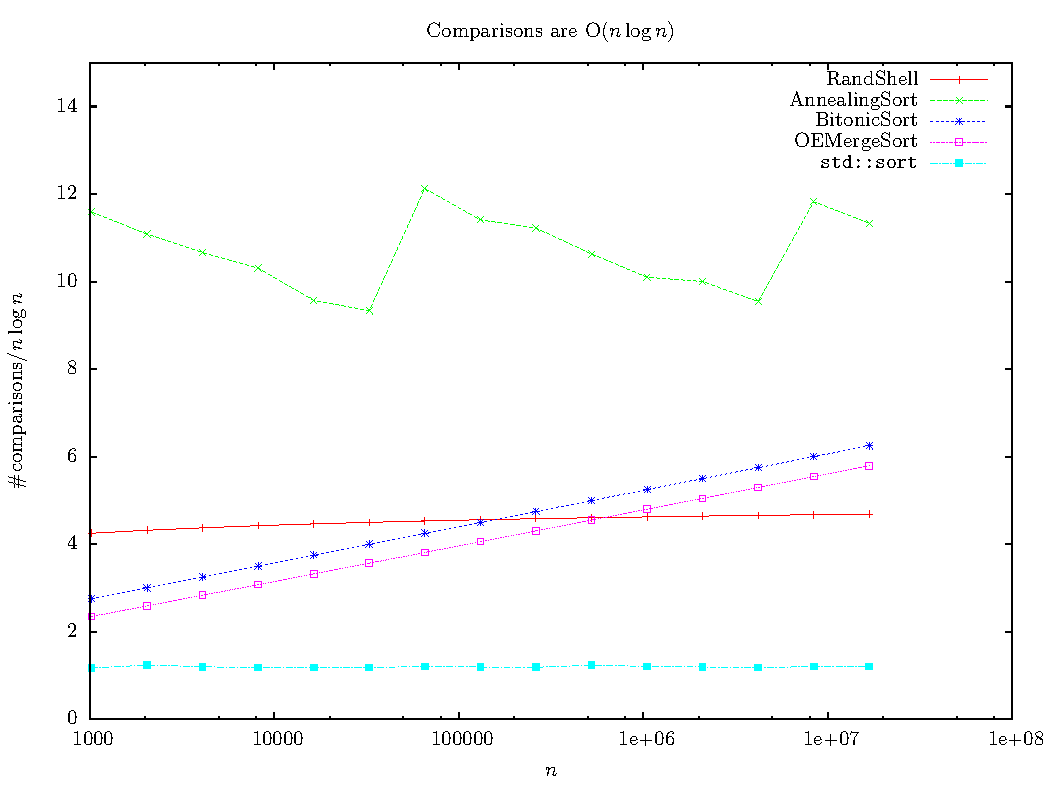
\includegraphics[width=\textwidth]{graphs/Performance/nlogncomparisons.pdf}
\caption{Comparison count of the algorithms}
\label{fig:Performance:comparisons}
\end{figure}


Now, let us look at the running times of the algorithms, which are shown in Figure~\ref{fig:Performance:time}.
Unfortunately, running times are nowhere near as predictable or consistent with theory as the amount of comparisons, but they are however of great practical importance.

Randomized Shellsort appears slow compared to the other algorithms, especially considering its low amount of comparisons compared to the sorting networks, and at input sizes larger than $1 \times 10^6$, it appears to grow faster than $O (n \log n)$. An explanation for the slow running time of Randomized Shellsort is given in Section~\ref{sec:PerformanceInstructions}. At sizes between $1.6 \times 10^4$ and $1 \times 10^6$, we see the expected running time of $O( n \log n)$, which is consistent with theory.

Both Bitonic Sort and Odd-Even Mergesort show good performance, but they are growing in $O ( n \log^2 n)$. We see that Odd-Even Mergesort is slower than Bitonic Sort, despite performing fewer comparisons, which is interesting. Unlike Randomized Shellsort and Annealing Sort, there appears to be no immediate problem of going beyond $1 \times 10^6$ elements for these two algorithms.

Annealing Sort is slow, as expected from the high number of comparisons. At sizes between $1.6 \times 10^4$ and $1 \times 10^6$, the algorithm follows the $O(n \log n)$ expected complexity well, but performance degrades rapidly at the $1 \times 10^6$ element mark. This performance degradation will, like that of Randomized Shellsort, be further discussed in Section~\ref{sec:PerformanceInstructions}.


\begin{figure}
\center
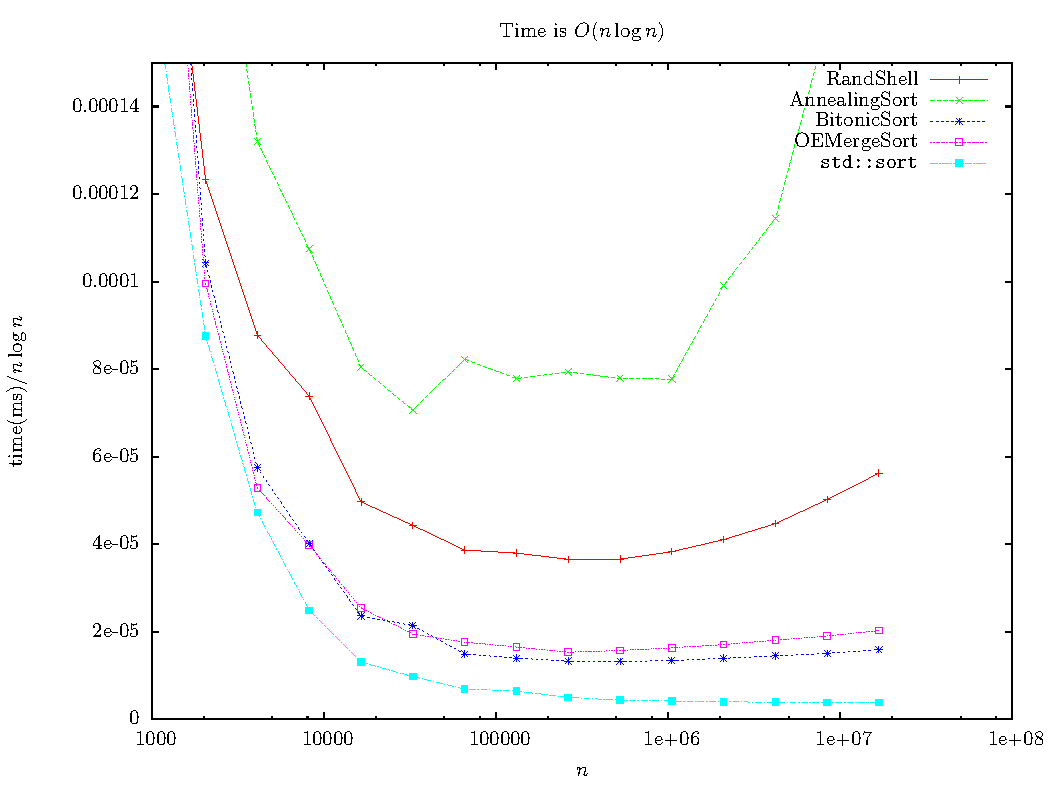
\includegraphics[width=\textwidth]{graphs/Performance/nlogntime.pdf}
\caption{Running time of the algorithms}
\label{fig:Performance:time}
\end{figure}


\subsection{Instructions and Cache Misses}
\label{sec:PerformanceInstructions}

Having shown that the algorithms behave somewhat reasonably, let us move on to show why performance is not directly tied to the number of comparisons, and why some algorithms run into problems at the $1 \times 10^6$ element mark.

First, let us look at the amount instructions performed per comparison, as shown in Figure~\ref{fig:Performance:instructions:comparisons}.
Note that all of algorithms converge towards a constant amount of instructions per comparison, which bodes well for their implementation.

We see that Randomized Shellsort has a high number of instructions per comparison, which helps explain why it is outperformed by the $O (n \log^2 n)$ sorting networks, despite having a similar or lower number of comparisons.

Bitonic Sort performs a low amount of instructions per comparison, which is what makes it outperform Odd-Even Mergesort despite using higher number of comparisons. The high number of instructions performed by the Odd-Even Mergesort can be atributed to the procedure of moving odd and even elements around between buffers.

Annealing Sort actually performs relatively few instructions per comparison, since it is a simple algorithm. This is unfortunately not enough to balance out the high number of comparisons in terms of final running time.

\begin{comment} %IM INVISIBRU
\begin{figure}
\center
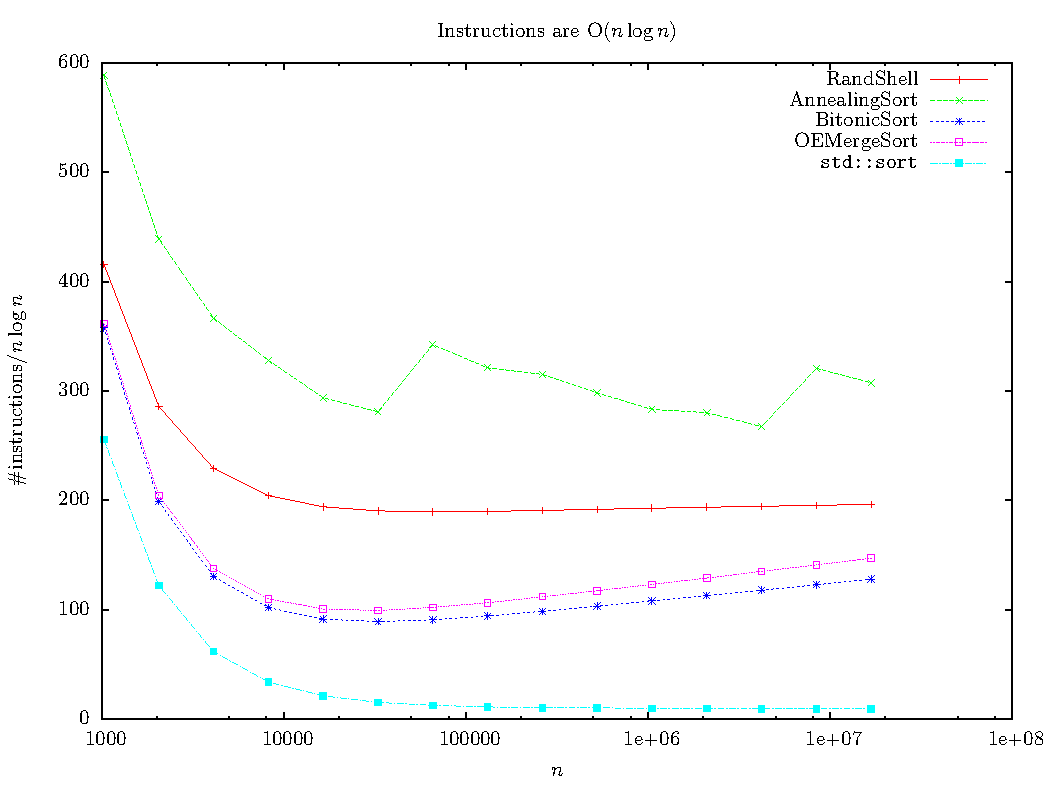
\includegraphics[width=\textwidth]{graphs/Performance/nlogninstructions.pdf}
\caption{Instruction Count of the algorithms}
\label{fig:Performance:instructions:nlogn}
\end{figure}
\end{comment}


\begin{figure}
\center
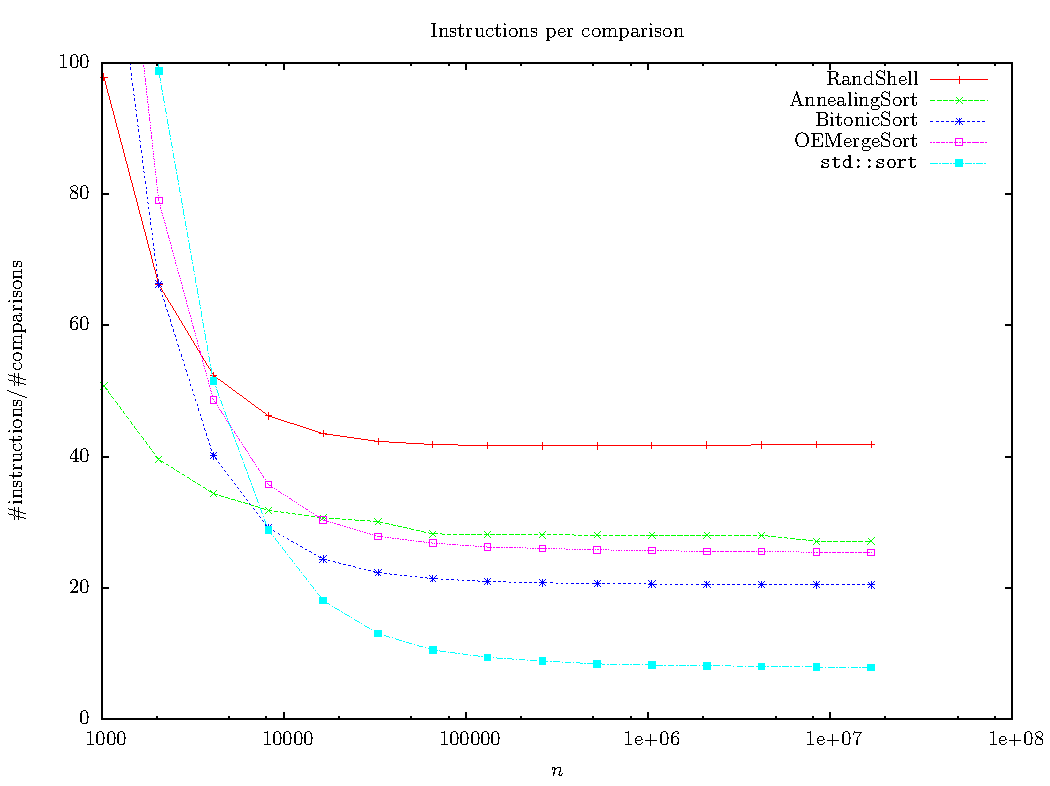
\includegraphics[width=\textwidth]{graphs/Performance/instructionscomparison.pdf}
\caption{Instructions per Comparison of performed by the algorithms}
\label{fig:Performance:instructions:comparisons}
\end{figure}

Now, let us move on to cache misses. Cache misses can be seen in Figure~\ref{fig:Performance:cachemisses}.
Keep in mind that test are performed on a machine with 4MB cache using signed 32-bit integers, which places the amount of elements fitting into cache at about $1 \times 10^6$ elements.

Randomized Shellsort and Annealing Sort both start having major cache problems around the cache limit, which explains their performance problems when going above  $1 \times 10^6$ elements. The high number fo cache misses is a direct effect of their random access patter when comparing data, which both prevents memory preloading, and leads to big jumps in accessed indexed of elements.

Bitonic Sort and Odd-Even Mergesort both perform few cache misses, since they both work locally in terms of data access, and rely on linear access patterns allowing the memory prefetcher to lower latency when crossing a cache line border.

\begin{figure}
\center
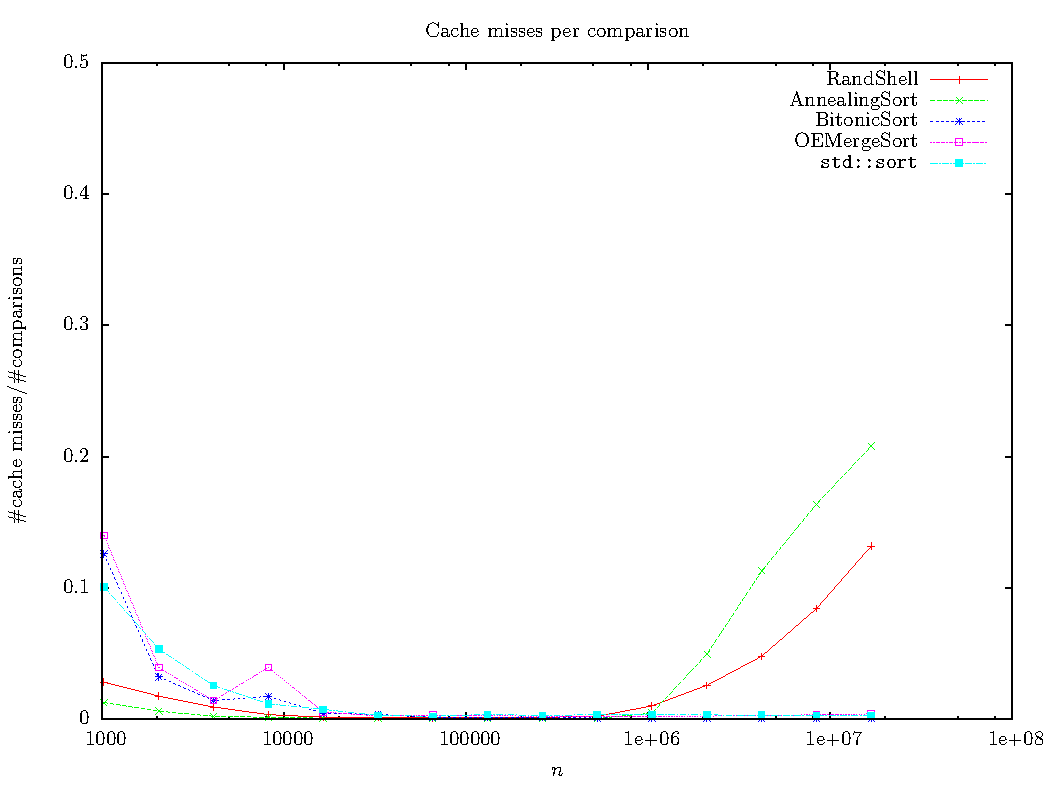
\includegraphics[width=\textwidth]{graphs/Performance/cache-misses.pdf}
\caption{Cache Misses of the algorithms}
\label{fig:Performance:cachemisses}
\end{figure}

\subsection{Branch Mispredictions}

Throughout this section, we have made many interesting observations about the data-oblivious algorithms, but unfortunately, they seem to be outperformed by \texttt{std::sort} on every single performance metric. Though there is still one point in which they can outperform classic data-dependent sorting algorithms.

Figure~\ref{fig:Performance:branchmisses} shows the number of branch mispredictions performed by the different algorithms.

The data-oblivious algorithms can all be seen to perform a number of branch mispredictions that is either almost negligible, or $O (n)$, since the \texttt{Compare-Exchange} operation can be done without branching. \texttt{std::sort}, on the other hand, performs a number of branch mispredictions that is $O(n \log n)$, since it is must perform a branch for each comparison, and assuming uniformly random input data, it will not be possible to reliably predict the result of this branch. 

\begin{figure}
\center
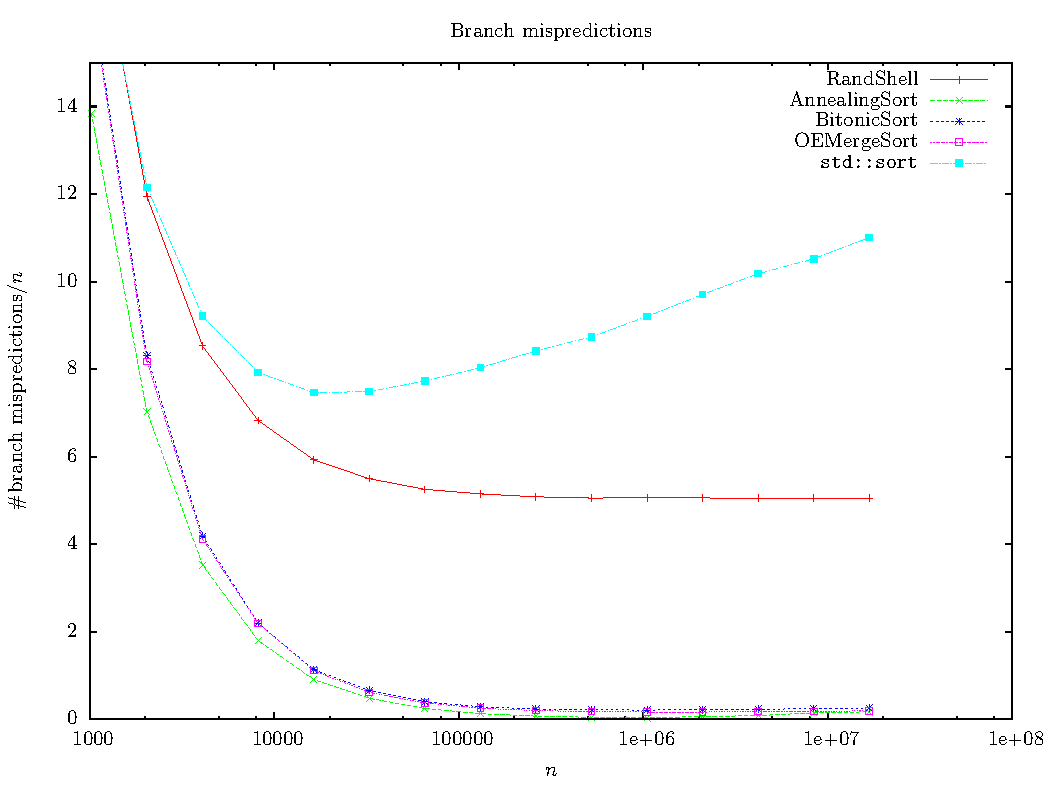
\includegraphics[width=\textwidth]{graphs/Performance/branch-misses.pdf}
\caption{Branch Mispredictions of the different algorithms}
\label{fig:Performance:branchmisses}
\end{figure}

\subsection{Experiment Results}

The experiment shows that both of the new algorithms perform according to their expected running times of $\Theta(n \log n)$, for a significant part of the experiment. These newer algorithms are however hindered by a large instruction overhead and a poor cache performance, and are therefore somewhat slow in practice.

Randomized Shellsort is notable in that it performs a low number of comparisons compared to Bitonic Sort and Odd-Even Mergesort as $n$ increases, which might prove useful in the field of secure multi-party computations.

Annealing Sort seems entirely unsuited for practical use.



\section{Evaluating Shellsort Variants}
\label{sec:ShellsortExperiments}

Since Section~\ref{sec:Performance} is already crowded, we have chosen to relocate the test for the different variants of Shellsort to this separate section.

The tests follow an identical set-up to the one presented in Section~\ref{sec:Performance}, using inputs that are a power of 2. Note that Shaker Sort, as mentioned in Section~\ref{sec:ShellsortImplementation}, will use a sequence consisting of numbers $\floor{1.7^j}+1 < n$ and two $1-shakes$ to finish, and since the input is randomly generated, the initial shuffle is omitted.

Bitonic Sort and \texttt{std::sort} are included for reference. 

\subsection{Running Time and Comparisons}

Let us first consider the amount of comparisons and time spent in order to sort the input, in order to verify the expected $\Theta(n \log n)$ and $O(n \log^2 n)$ complexities of the algorithms. This will, like the previous performance test, show us a great deal about the basic properties of the algorithm, and the overhead associated with execution the algorithm.

Let us begin by considering the number of comparisons performed.

Pratt's Shellsort can be seen performing a number of comparisons that is both $O(n \log ^2 n)$ and slightly larger than that of Bitonic Sort. This is a noted property from~\citeA{PrattThesis}, and the experiment confirms this.

Shaker sort performs an impressively low amount of comparisons, especially when compared to Randomized Shellsort, representing another take at $\Theta(n \log n)$ Shellsort variations. Given the $\floor{1.7^j}+1$ jump sequence of Shaker Sort, we expect the constant factor for the algorithms to be around $2\cdot \log(1.7)^{-1} \approx 2.6$, which fits the experimental results.

\begin{figure}
\center
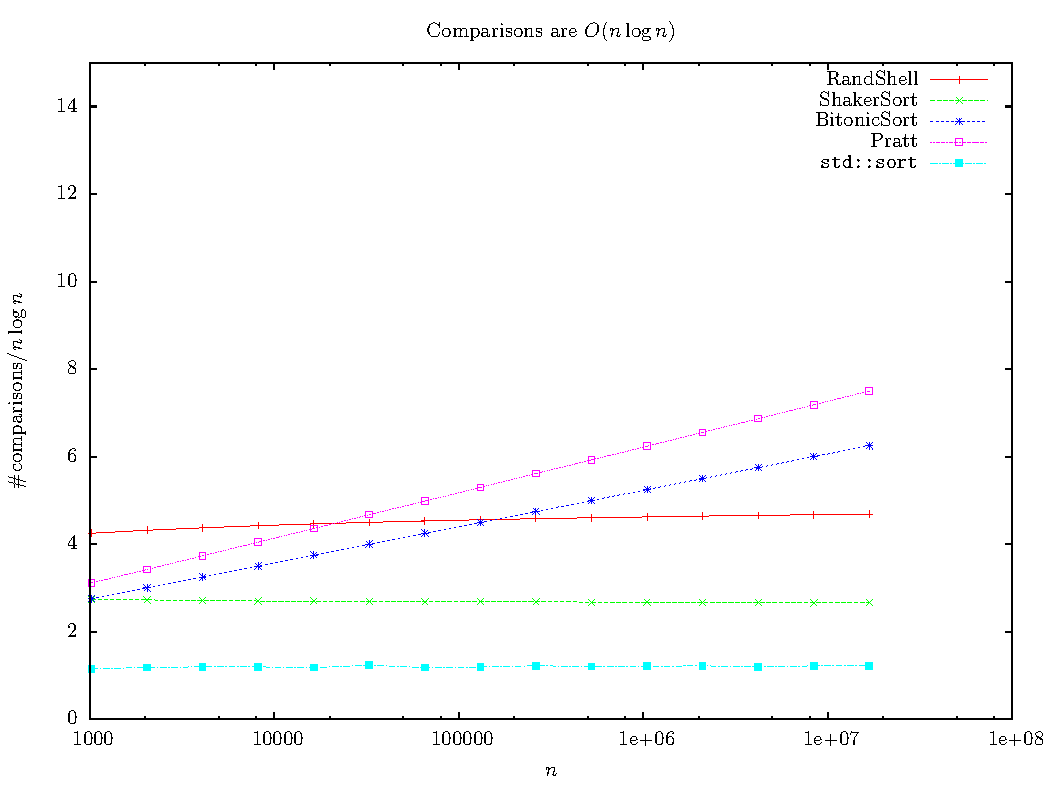
\includegraphics[width=\textwidth]{graphs/Shellsorts/nlogncomparisons.pdf}
\caption{Comparison count of the algorithms}
\label{fig:Shellsorts:comparisons}
\end{figure}

Let us then look at the running time of the algorithms, to ensure that no strange overhead is involved in sorting the data.

We see Pratt's Shellsort perform slightly worse than Bitonic Sort, but still $\Theta(n \log^2 n)$, which can be explained by a higher number of \texttt{Compare-Exchange} operations.

Shaker Sort shows great potential, performing much better than both the $\Theta(n \log^2 n)$ algorithms and Randomized Shellsort. This places Shaker Sort in a favourable position for further optimizations by applying parallel execution schemes. Keep in mind though, that the unknown failure rate for Shaker Sort might make it less desirable for practical use.
 
\begin{figure}
\center
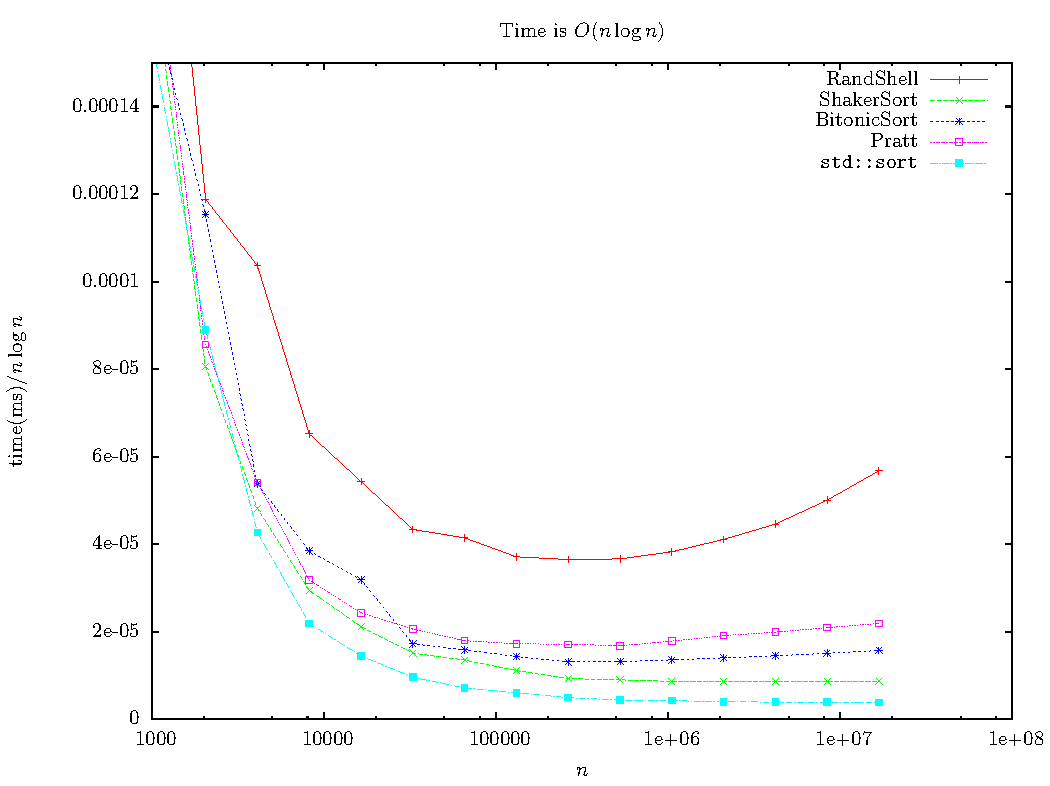
\includegraphics[width=\textwidth]{graphs/Shellsorts/nlogntime.pdf}
\caption{Running time of the algorithms}
\label{fig:Shellsorts:time}
\end{figure}

\subsection{Instructions and Cache Misses}

Now, let us look at the constant factors involved in the two Shellsort variants, and determine whether cache performance might become a problem for larger inputs, or if some of the algorithms might have an overly large instruction overhead.

Let us start by evaluating the amount of instructions per comparisons, in order to gain an insight into the performance overhead of the algorithms.

We see Pratt's Shellsort perform an amount of instructions per comparison that is slightly lower than that of Bitonic Sort, and much lower than Randomized Shellsort, while Shaker Sort is almost identical to Bitonic Sort in terms of instructions per comparison.
The low comparison overhead of the two Shellsort variants is made possible by most of their execution consisting of a few nested for-loops. 
They do however suffer from a difficulty in loop unrolling due to having their jump sequences calculated at run-time. 

\begin{figure}
\center
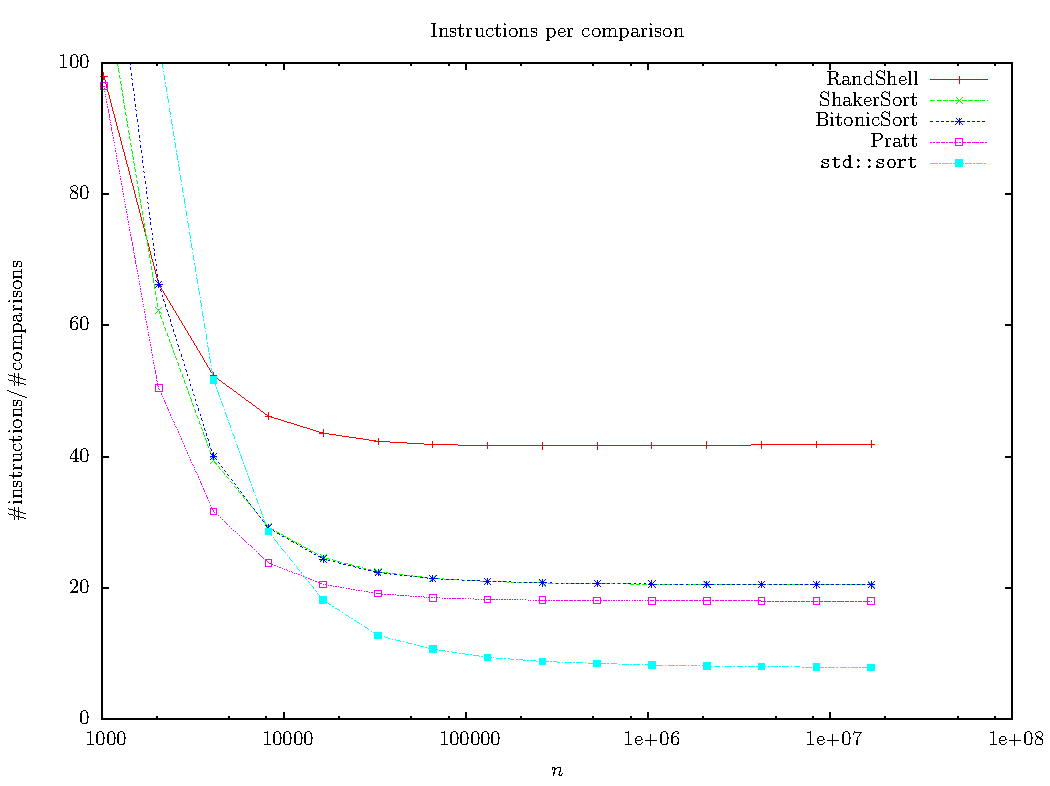
\includegraphics[width=\textwidth]{graphs/Shellsorts/instructionscomparison.pdf}
\caption{Instructions per Comparison of performed by the algorithms}
\label{fig:Shellsorts:instructions:comparisons}
\end{figure}

When looking at cache misses, we see no immediate rise in the amount of cache misses per comparison for the Shellsort variants when hitting the cache limit. This is as expected, since both of these variants of Shellsort relies entirely on performing one or two linear two-headed scans through memory per offset in the jump sequence.

\begin{figure}
\center
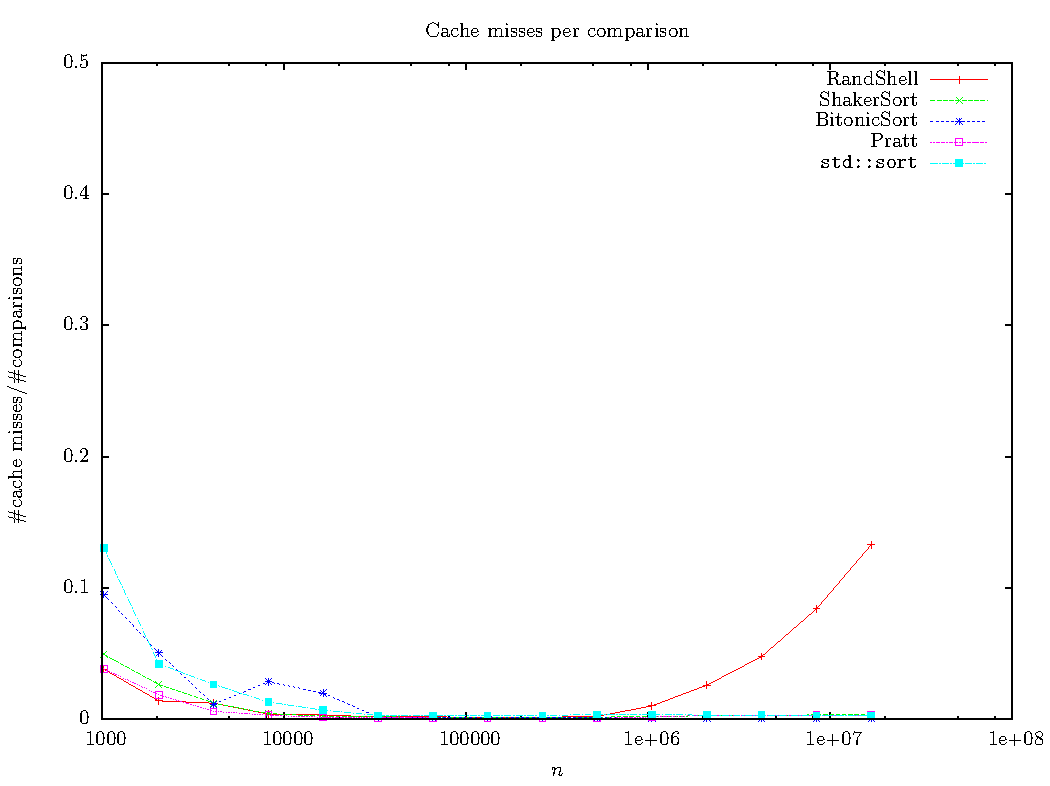
\includegraphics[width=\textwidth]{graphs/Shellsorts/cache-misses.pdf}
\caption{Cache Misses of the different algorithms}
\label{fig:Shellsorts:cachemisses}
\end{figure}

\subsection{Branch Mispredictions}

Again, let us look at the number of branch mispredictions for our data-oblivious algorithms, as they are  shown in Figure~\ref{fig:Shellsorts:branchmisses}.

We see Pratt's Shellsort and Shaker Sort perform the low amount of branch mispredictions that we have come to expect from the first experiment. Again, this is a desirable property of the algorithms when we must consider them for parallel optimization schemes.

\begin{figure}
\center
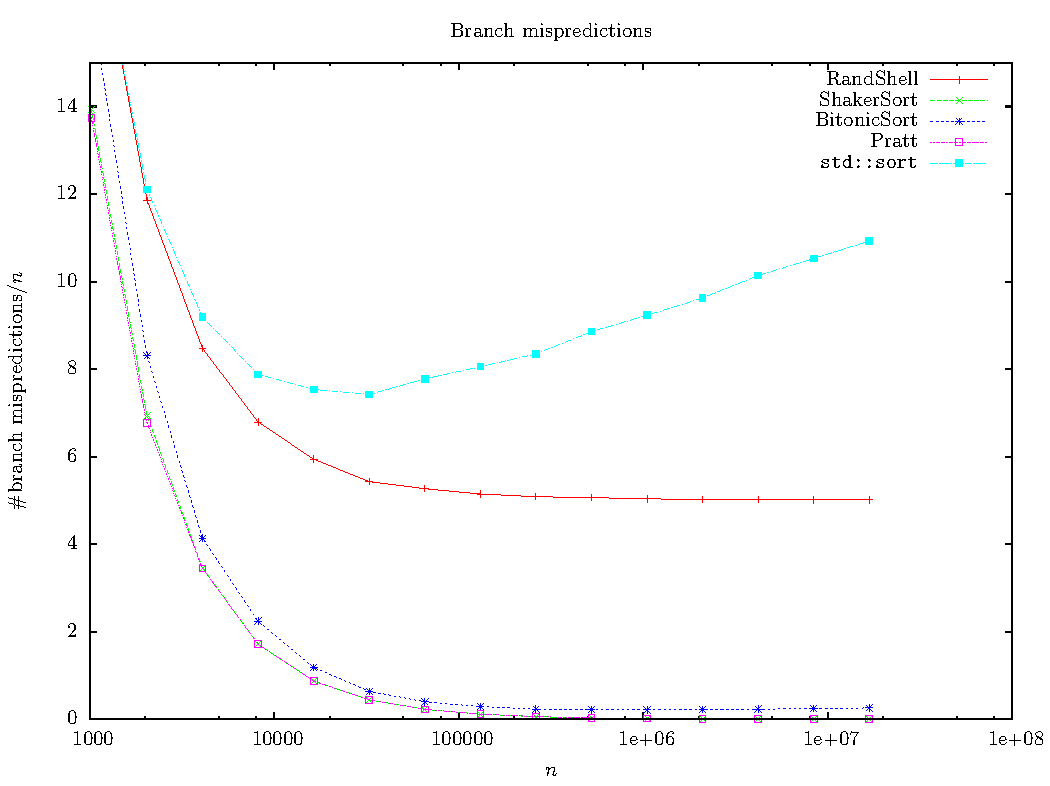
\includegraphics[width=\textwidth]{graphs/Shellsorts/branch-misses.pdf}
\caption{Branch Mispredictions of the different algorithms}
\label{fig:Shellsorts:branchmisses}
\end{figure}

\subsection{Experiment Results}

The experiment shows that both Pratt's Shellsort and Shaker Sort have excellent performance characteristics.

Pratt's Shellsort is slightly slower than Bitonic Sort, but this a by a small margin, which is a symptom of performing a slightly higher amount of comparisons.

Shaker Sort is shown to be fast in practical applications, and might be a useful data-oblivious algorithm if one ensures somewhat random input data, or accepts an unknown failure rate on certain input instances.

 \FloatBarrier
\section{Finding Good Constants for Annealing Sort}
\label{sec:AnnealingExperiments}

Annealing Sort will, in the state that it is described in~\citeA{AnnealingSort}, sort any given input with a very high probability, but the parameters given for the different parts of the annealing sequence result in an exceptionally slow sorting algorithm.

These constants are, like those of Randomized Shellsort, mostly an artefact of an overly pessimistic analysis, and this section will show an experimental exploration of suitable parameters.

The two parameters under test are $g_{scale}$, and $h$, where $g_{scale}$ directly modifies $g$ such that the length of the third part of the annealing sequence is $\floor*{g_{scale} \times 64e^2 \log n} + 1$ , and $h$ is used in determining $r$, so that $r = \floor*{h \times \frac{\log n}{\log \log n}}$.
The values of $c$ and $q$ are not considered, as they only become relevant at larger data sizes than those considered in the experiments.

Each test is performed by running the algorithm with a given set of parameter on 100 randomly generated inputs of fixed length.

\subsection{Sorting Effectiveness}

At first, let us consider how well the algorithm sorts, as lowering the constants below the level where the algorithm has a reasonable chance of sorting would be counter-intuitive.

Figure~\ref{fig:Annealing:percent1024} and~\ref{fig:Annealing:percent8192} show maps of the failure rate for $n = 1024$ and $n = 8192$ using varying values for $h$ and $g_{scale}$.
From this data, we see that both parameters influence the data in their own way.

For changing values of $g_{scale}$, we see that for a matching $h$ parameter, there will be a sweet spot where the failure rate quickly decreases from 100\% to 0\%, but this sweet spot moves as we increase $n$ or $h$. We also find that higher values of $h$, the $g_{scale}$ parameter can be set to $0$ leading to only a single pass during the last part of the annealing sequence.

For varying values of $h$ we see that it is highly dependent on flooring after multiplication by the logarithmic fraction, which leads to 'stepping' in the failure rate dependent on $n$. We also see that choosing a value of $h$ in the high end of the spectrum of testing values will lead low failure rates. Especially interesting is the fact that for $n = 8192$, $h$ values greater than $0.6$ leads to a failure rate of 0 independent of the value of $g_{scale}$.

\begin{figure}
\center
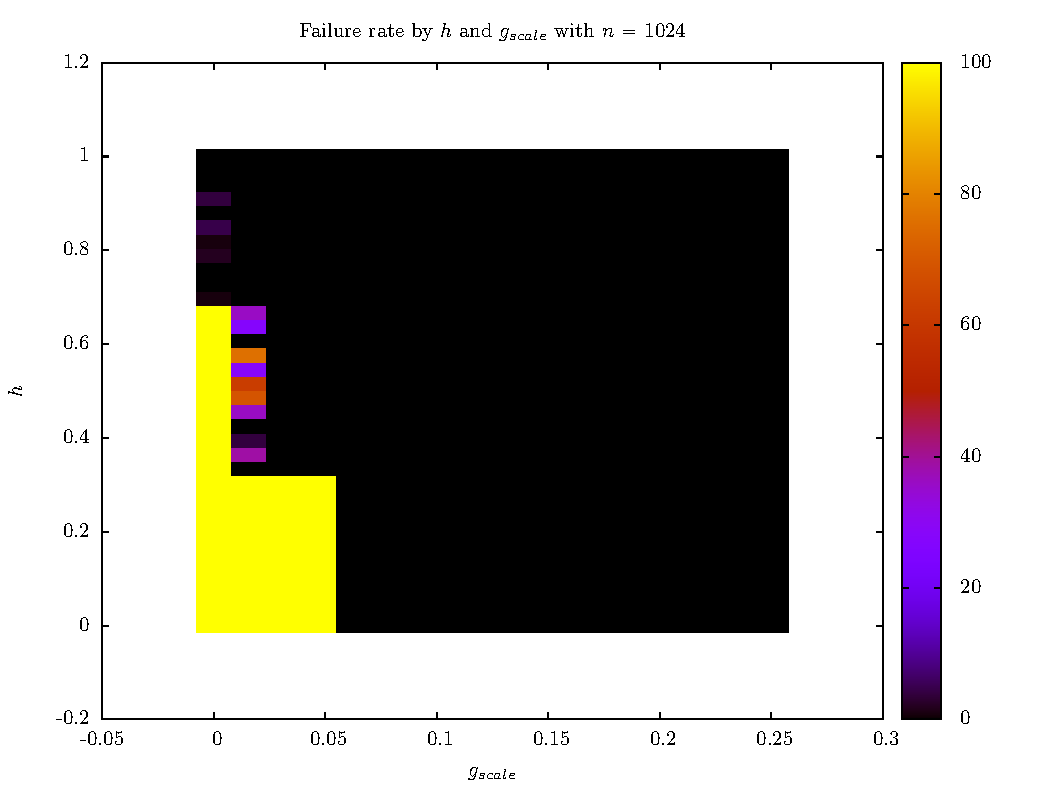
\includegraphics[width=\textwidth]{graphs/Annealing/annealing1024percent.pdf}
\caption{Failure rate of Annealing Sort with $n = 1024$}
\label{fig:Annealing:percent1024}
\end{figure}

\begin{figure}
\center
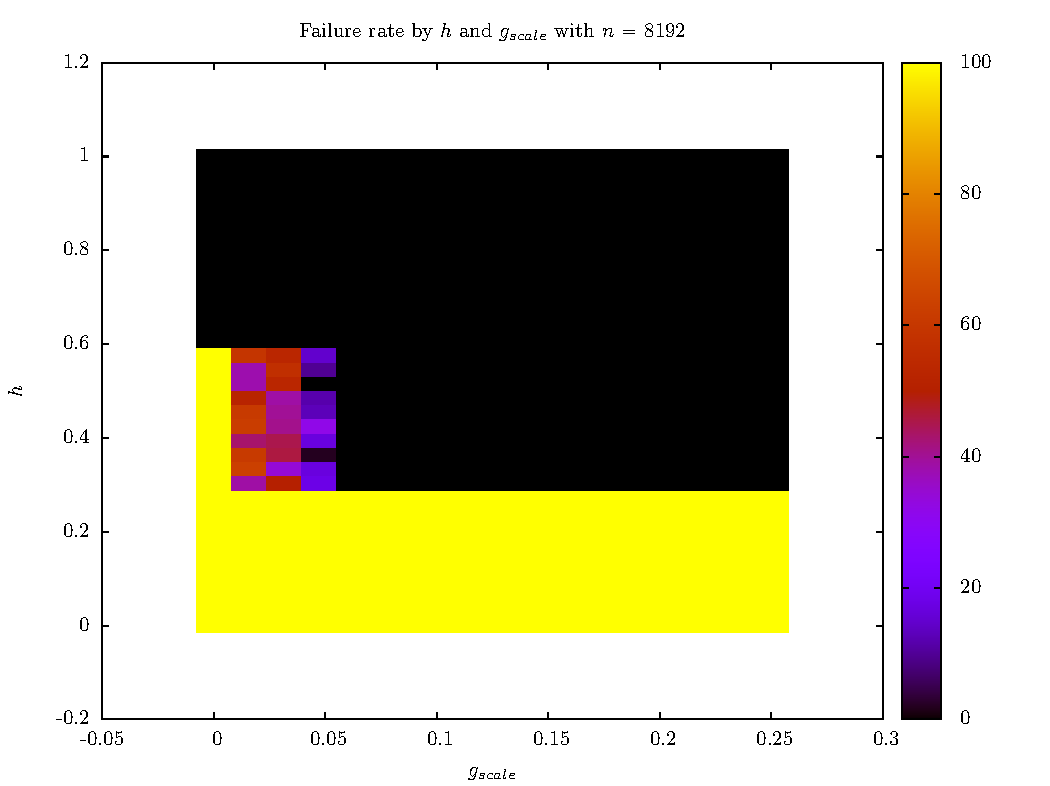
\includegraphics[width=\textwidth]{graphs/Annealing/annealing8192percent.pdf}
\caption{Failure rate of Annealing Sort with  $n = 8192$}
\label{fig:Annealing:percent8192}
\end{figure}

\subsection{Running Time}

Having investigated how failure rate depended on $h$ and $g_{scale}$, let us consider their effect on running time. Figure~\ref{fig:Annealing:time1024} and~\ref{fig:Annealing:time8192} show a map of running time with varying values of $h$ and $g_{scale}$.

From these maps we see that running time is clearly dominated by the contributions on the last phase, and the lower we scale its length, the better the running time. In fact, for both data sizes, it is almost impossible to spot the minor impact of increasing $h$, but it should be noted that it is definitely there, just rather minor compared to the great effect of $g_{scale}$.

\begin{figure}
\center
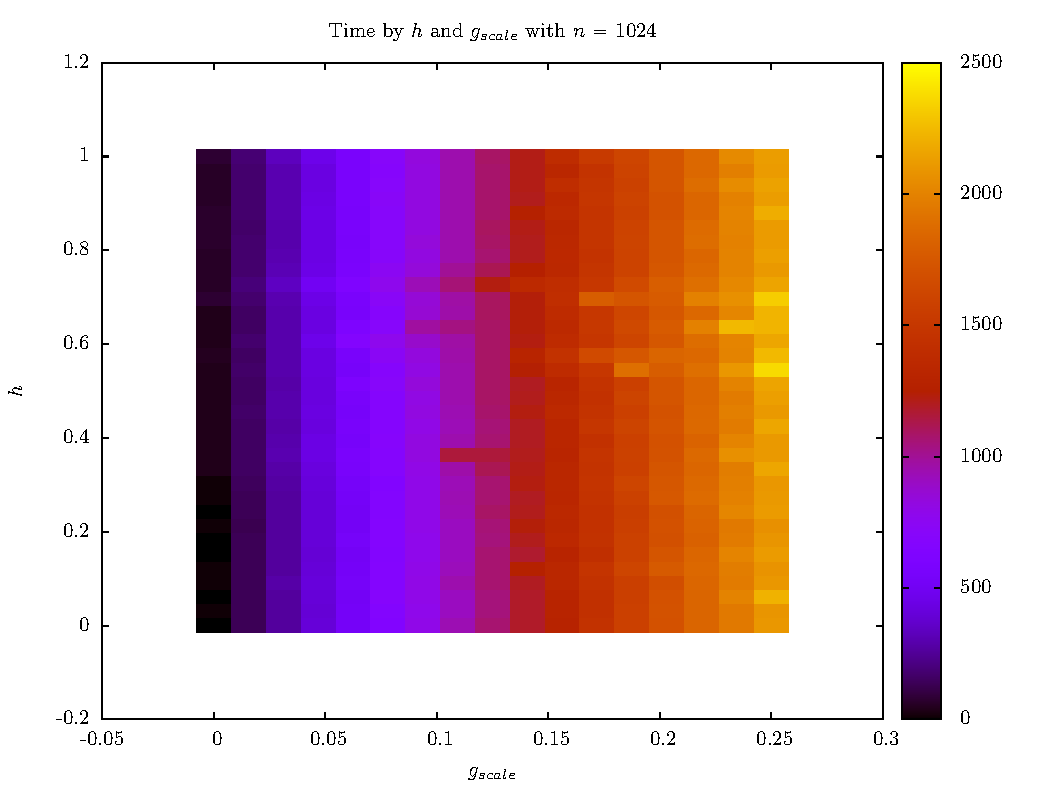
\includegraphics[width=\textwidth]{graphs/Annealing/annealing1024time.pdf}
\caption{Running time of Annealing Sort with  $n = 1024$}
\label{fig:Annealing:time1024}
\end{figure}

\begin{figure}
\center
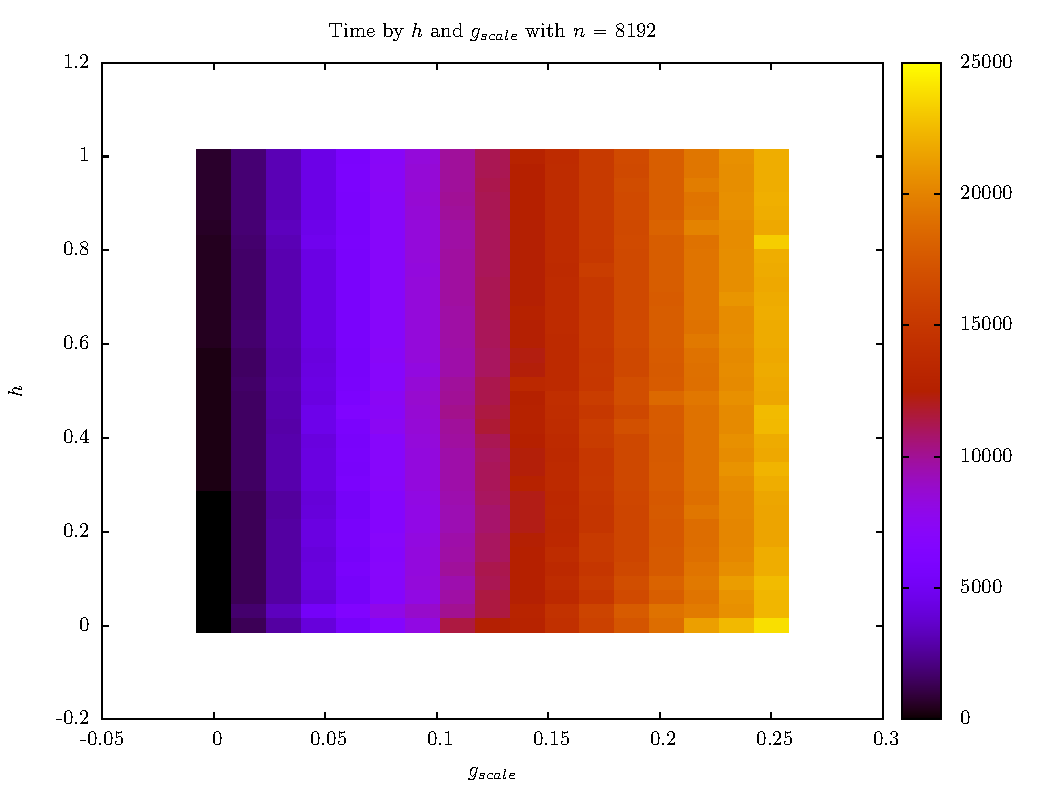
\includegraphics[width=\textwidth]{graphs/Annealing/annealing8192time.pdf}
\caption{Running time of Annealing Sort with $n = 8192$}
\label{fig:Annealing:time8192}
\end{figure}

\subsection{Large $n$}

From the previous experiments we learn two important lessons about the parameters used in constructing the annealing sequence for Annealing Sort;

\begin{enumerate}
\item Keep $h$ high, for a low dependable failure rate.
\item Keep $g_{scale}$ low, for a faster running time.
\end{enumerate}

Using this knowledge, we find the values of $h = 1$ and $g_{scale} = 0$ to be likely candidates for a speedy, reliable version of Annealing Sort.
In order to verify that these values does indeed sort with a high probability, tests were done using these parameters, and large values of $n$, which gave the following results:

\begin{table}[!ht]
\begin{adjustwidth}{-.5in}{-.5in}
\centering
\begin{tabular}{|l|c|c|c|c|c|c|c|c|c|c|c|}
\hline
n      & 1024 & 2048 & 4096 & 8192 & 16384 & 32768 & 65536 & 131072 & 262144 & 524288 & 1048576 \\ \hline
errors & 0    & 0    & 0    & 0    & 0     & 0     & 0     & 0      & 0      & 0      & 0       \\ \hline
\end{tabular}
\caption{Annealing Sort errors for large $n$, from 100 runs}
\end{adjustwidth}
\end{table}

From these results, we assume that these parameters are sufficient in providing a low failure rate, and their use in other experiments can be accepted.

\subsection{Experiment Results}

The experiment shows that using different parameters for Annealing Sort than those suggested in~\citeA{AnnealingSort} can improve the performance of the algorithm without negatively affecting the failure rate. 
This makes for a much faster version of Annealing Sort for use in practical applications.

\FloatBarrier
\section{Cache Performance of Odd-Even Merge Sort}
\label{sec:OEMergesortExperiment}

In Section~\ref{OEMergesortImpl} it is claimed that Odd-Even Mergesort benefits heavily from using an additional $\Theta(n)$ storage as a buffer to permute elements into a more memory-local ordering. Note that any efficient in-place permutation could easily replace this buffer, but efficient solutions for this problem do not appear immediately feasible.

Let us quickly reiterate what the problem is. Odd-Even Merging requires recursive calls to work on odd and even indices separately, which is often represented by providing a distance between elements to consider at the current level of the merge. This will however completely thrash the CPU cache by accessing elements in separate cache lines, leading to a massive performance degradation when data sizes grow beyond what fits into to last cache layer.
Swapping data back and forth between a buffer easily solves this problem, at the cost of a higher instruction count and memory usage.

Additionally, we have the opportunity to perform multiple layers of the recursive calls in each scan through the memory between each permuting step, which could lead to a reduction in cache misses.

The tests are performed in the same way as those of Section~\ref{sec:Performance}, but compares three executables, one using a buffer for Odd-Even Mergesort, one using a buffer and performing 2 layers of operation per re-ordering, and one having it disabled.

\subsection{Running Time and Cache Misses}

Figure~\ref{fig:Buffer:tc} shows the running time of the algorithm variants overlaid with the amount of cache misses per comparison performed. 
This shows a big difference in the amount of cache misses incurred between the buffered and unbuffered variants, and highlights the corresponding increase in running time for the unbuffered version of Odd-Even Mergesort. 
Note that the increase in running time makes the algorithm grow asymptotically faster than $O(n \log^2 n)$ for inputs larger than the CPU cache, while the buffered variants shows a running time that is much more consistent with the running time suggested by the standard RAM model.
There seems to be almost no difference in running time between the single-layered and double-layered buffering variants.

\begin{figure}
\center
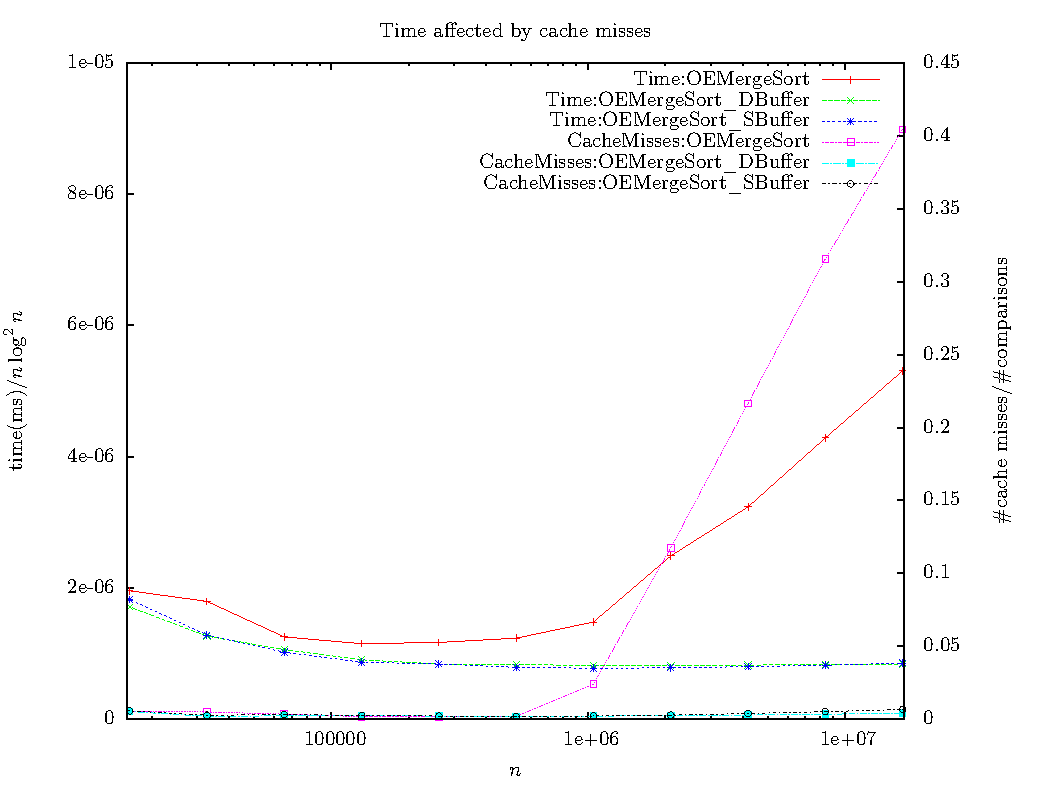
\includegraphics[width=\textwidth]{graphs/Buffer/tc.pdf}
\caption{Time overlaid with cache misses}
\label{fig:Buffer:tc}
\end{figure}


When looking at Figure~\ref{fig:Buffer:tc}, it is also clear that the unbuffered variant of Odd-Even Mergesort grows faster than $O(n \log^2 n)$ even for values well within the cache limit.
This observation might seem strange at first, but Figure~\ref{fig:Buffer:tc2} will show a reasonable explanation for this being the L1 cache layer. In the aforementioned figure, we can see the running time overlaid with the amount of L1 cache load misses. The L1 cache is much smaller than the total CPU cache, and the latency between L1 and the outer cache layer is much smaller than the main memory latency, but still significant. We see that the unbuffered variant of Odd-Even Mergesort incurs  a lot more L1 load misses, which will unfavourable affect running time, and helps explaining why it is slower, even within cache limits.

The single-layered and double-layered variants show a significant difference in L1 cache load misses, but not much of a difference in running time. This is caused by the extra complexity required to compute the double-layered indices counter-acting the performance gained from a slightly reduced number of L1 cache misses.

\begin{figure}
\center
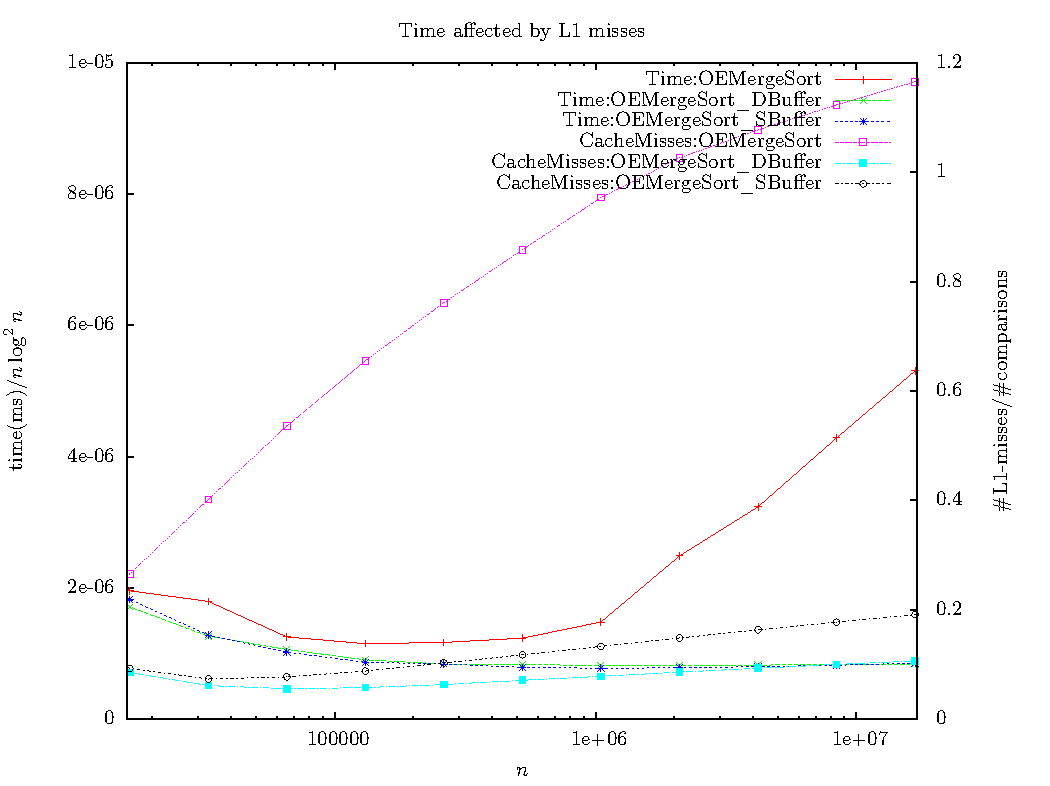
\includegraphics[width=\textwidth]{graphs/Buffer/tc2.pdf}
\caption{Time overlaid with cache misses}
\label{fig:Buffer:tc2}
\end{figure}


\subsection{Experiment Results}

The experiment show that moving data around in preparation to the recursive calls of the Odd-Even Merging does indeed have a large and measurable effect on performance. This shows that one must take care when implementing sorting networks directly on the CPU and justifies our solution of using buffers. 
Additionally, we can see that the two-layered cache-reordering strategy is feasible, but is not much better than performing a single layer per reordering. The lower amount of L1 cache misses, combined with an almost identical running time makes it favourable, but this might change depending on the development in cache speed versus instruction speed. 


\FloatBarrier
\section{Branch Behaviour of Compare-Exchange Variants} \FloatBarrier
\label{sec:CEBranchExperiment}


In Section~\ref{sec:CompareExchangeImpl} we describe different ways implementing the \texttt{Compare-Exchange} operation in such that it is possible to both eliminate the need for branches and pipeline dependencies on conditional moves.

Measuring the effect of pipeline halts from conditional moves is difficult, and their impact is heavily dependent on the underlying architecture. As such, they are to be avoided, but we will unfortunately not be able to base this on much more than good faith.

Branch mispredictions on the other hand are easily measurable and fitting for experimentation.
We measure the branch misprediction rate by running the algorithms using both the branching variant and the \texttt{xor} variant of the \texttt{Compare-Exchange} operation, subtracting the number of branch mispredictions from the \texttt{xor} variant, and divide by the number of comparisons. The reasoning for this way of obtaining branch misprediction rate being that using \texttt{xor}, we obtain the number of branch mispredictions from the overhead instructions of the algorithms, and any mispredictions that exceed this number should be caused only by comparisons.

We note that there might be some collisions in predictions between overhead and comparisons, but on a modern processor, this should be minor, especially due to the low number of branch mispredictions normally incurred by the overhead of the algorithms, as observed in Figure~\ref{fig:Performance:branchmisses} and~\ref{fig:Shellsorts:branchmisses}. 

We observe that algorithms behave differently in terms of branch misprediction rates of comparison. Note that an optimal sorting algorithm for unknown random inputs should mispredict about $50\%$ of all comparisons.

The tests are performed in the same way as those of Section~\ref{sec:Performance}, but compares two executables, one using the \texttt{xor}-based \texttt{Compare-Exchange}, and the other using the branching variant based on \texttt{std::swap}.

\subsection{Results}

\begin{figure}
\center
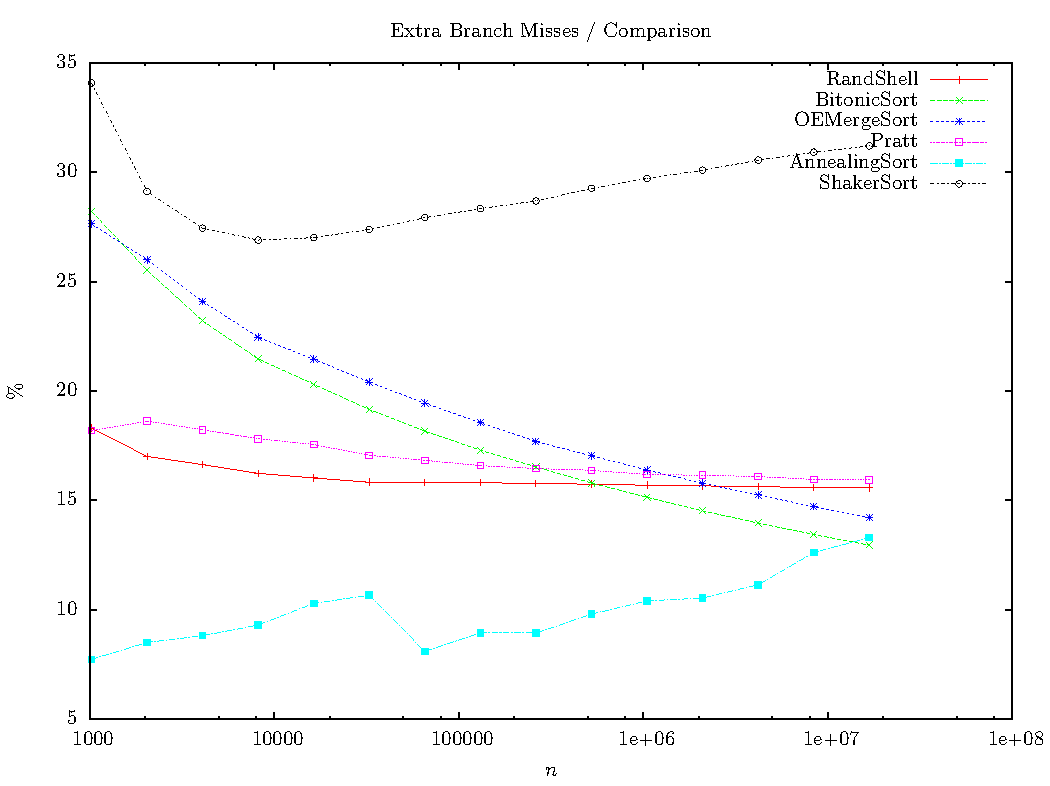
\includegraphics[width=\textwidth]{graphs/CompareExchange/branchdiff.pdf}
\caption{Branch Mispredictions of the different algorithms}
\label{fig:CompareExchange:branchdiff}
\end{figure}

Figure~\ref{fig:CompareExchange:branchdiff} shows how many of the additional branches imposed by having a data-dependent \texttt{Compare-Exchange} actually result in a branch-misprediction.

Randomized Shellsort shows a constant, but low amount of branch mispredictions. This is likely due to the fact that it makes a large random amount of comparisons, while being asymptotically optimal.

Annealing Sort also shows a low number of branch mispredictions, most likely due to performing a large amount of comparisons. As $n$ grows, we see the misprediction rate grow slightly, which might be caused by the algorithm moving slightly closer to the minimum amount of comparisons.

Bitonic Sort and Odd-Even Mergesort start off with a high number of branch mispredictions, but this number decreases as $n$ grows. This drop in misprediction is most likely caused by the additional $\Theta(\log n)$ factor of comparisons performed. When considering Bitonic Sort, the merging step will be especially graceful in branch mispredictions, as we should see them only when the two halves of the bitonic sequences cross.

Pratt's Shellsort is somewhat strange. It performs a non-optimal amount of comparisons, yet shows little improvement as $n$ increases, though it also starts low. What causes this is hard to predict, but it might be due to the way Shellsort variants often compare far-apart elements, as opposed to the somewhat local merges of Bitonic Sort and Odd-Even Mergesort

Finally, we have Shaker Sort. Shaker Sort seems to express a high and slightly growing amount of branch mispredictions. A plausible explanation for this is the close-to-optimal amount of comparisons made by Shaker Sort, and as $n$ grows, the impact of the final 1-shakes somewhat gets dampened by the growing amount of offsets in the jump sequence. Should $n$ grow fairly large, we would most likely see Shaker Sort converge towards some constant somewhere between $35$ and $50$ percent. 

\subsection{Experiment Results}

The experiment showed that one must indeed take care when implementing a \texttt{Compare-Exchange} operation on the CPU, as it will induce a large amount of branch mispredictions if it is not data-oblivious. With the big pipelines present in modern CPU architectures, this might become important.

Also, we see that the different algorithms perform a highly variable, and not always predictable, amount of branch mispredictions, as input sizes grow.

\FloatBarrier
\section{SIMD Experiments}
\label{sec:SIMDExperiments}
Section~\ref{sec:SIMDImpl} describes how to use the new SSE4.1 instruction set to speed up the operation of data-oblivious sorting algorithms.
In this section, we show how performance is affected in real-life implementations of the algorithms, and show how different usages of the SIMD architecture can make or break the performance gain.
These experiments we focus on the instruction count and running time, as these are the only metrics that change noticeably when using SSE.

Note that performing two recursive calls in a single scan is not beneficial when using SIMD, so Odd-Even Mergesort will only use the simple buffering strategy.

\subsection{Instructions}

The immediate effect of using SSE instructions is a significant reduction in the amount of operations required per comparison, due to having 4-way comparisons and intrinsic \texttt{min}/\texttt{max} operations. Figure~\ref{fig:SIMD:instructions} and~\ref{fig:SIMD:instructions:comparisons} show the total amount of instructions, and the number of instructions per comparison.

Both Randomized Shellsort and Odd-Even Mergesort show a reasonable reduction in instruction count, but overhead from the general operations of the algorithms overshadow the amount of operations tied up comparisons.

Bitonic Sort shows a massive reduction in instruction count from the application of SIMD instructions. The massive gain for Bitonic Sort stems from the low instruction overhead of the algorithm, since the benefit of using SIMD is heavily dependent on the amount of operations dedicated to comparisons.

Pratt's Shellsort and Shaker Sort also both show a big impact from SIMD in the number of instructions performed. This big reduction in the amount of instructions is most likely caused by the structure of the algorithms being based entirely on nested for-loops. No extra instructions are spent setting up recursive calls. Especially noteworthy is the low instruction count of Shaker Sort, combined with an $O(n \log n)$ running time.

\begin{figure}
\center
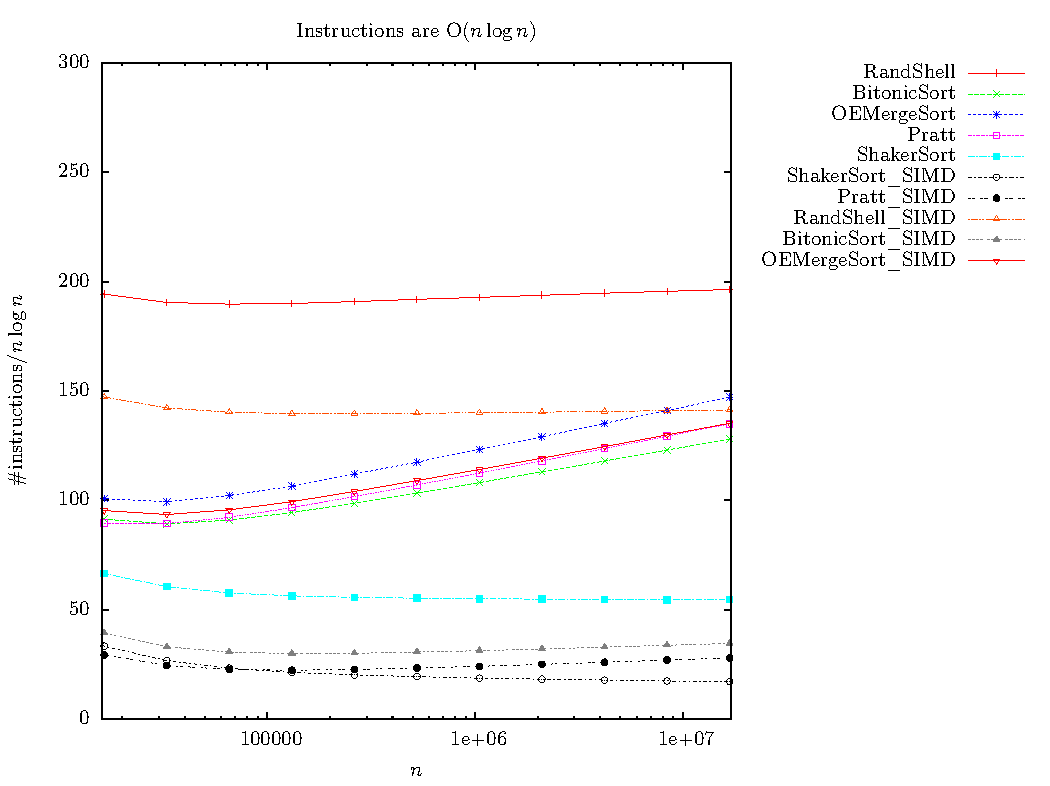
\includegraphics[width=\textwidth]{graphs/SIMD/nlogninstructions.pdf}
\caption{Instruction count with and without SIMD}
\label{fig:SIMD:instructions}
\end{figure}


\begin{figure}
\center
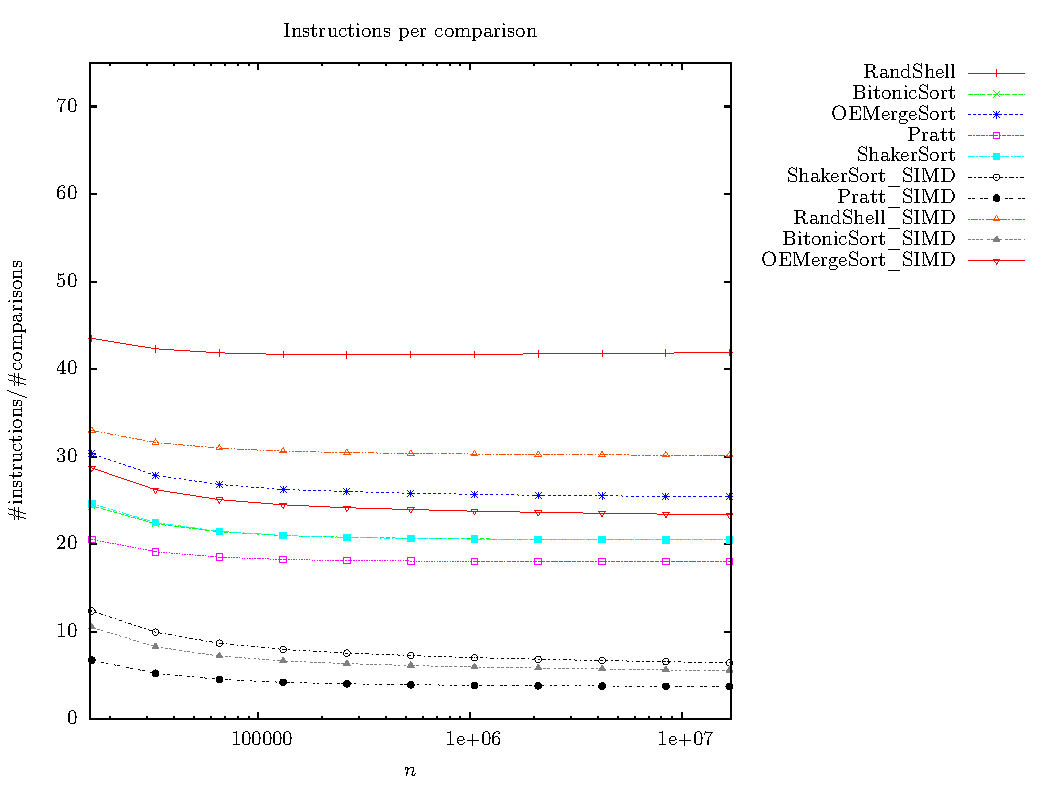
\includegraphics[width=\textwidth]{graphs/SIMD/instructionscomparison.pdf}
\caption{Instructions per comparison count with and without SIMD}
\label{fig:SIMD:instructions:comparisons}
\end{figure}

\subsection{Time}

Having shown the impact on the instruction count when using SSE operations, let us consider the actual performance gain.

In Figure~\ref{fig:SIMD:time} we can see the actual running times, while Figure~\ref{fig:SIMD:timediff} shows the performance gain. Table~\ref{tab:SIMD:timediffavg} shows the mean performance gain, as obtained from the data shown in Figure~\ref{fig:SIMD:timediff}.

Randomized Shellsort shows a small but noticeable gain from SSE instructions. The problem of using SIMD with Randomized Shellsort comes from the need to fetch data into the SSE registers from separate locations in the memory due to the random nature of the region comparison procedure.

Odd-Even Mergesort shows a small but noticeable improvement from SSE instructions. Odd-Even Mergesort has much more linear memory access patterns than Randomized Shellsort, but they are unfortunately often shifted away from 16-byte boundaries of memory, which prevents optimal SSE load behaviour. 

Bitonic Sort shows a massive improvement in running time when using SSE instructions. This stems from the low overhead of the algorithm, coupled with fully linear 16-byte aligned memory access patterns. 

Shaker Sort shows a low running time, and a good improvement in running time from utilizing SSE instructions. Pratt's Shellsort also shows a good utilization of SIMD, but degrades rapidly at the cache limit on large inputs. Figure~\ref{fig:SIMD:timediff} also shows an unstable impact of SIMD to Pratt's Shellsort. We have no evidence pointing to a single source causing the degradation in Pratt's Shellsort at larger input sizes, but the fact that Shaker Sort shows a similar but smaller impact at a similar size, which lies close to the cache limit, suggests un-aligned SIMD accesses outside of the cache as a possible cause. The sizes of the subsequences processed by Pratt's Shellsort are not monotonically ascending, as they are for Shaker Sort, and this causes the algorithm to continously switch between SIMD and sequential execution, which is another possible cause for the degradation in performance.

\begin{table}[!h]
\begin{adjustwidth}{-.5in}{-.5in}
\centering
\begin{tabular}{|l|c|c|c|c|c|}
\hline
Algorithm & Randomized Shellsort & Bitonic Sort & Odd-Even Mergesort & Pratt & Shaker Sort \\ \hline
Factor    & 1.08                 & 2.81         & 1.12 & \textcolor{red}{2.87} & \textcolor{red}{2.16}              \\ \hline
\end{tabular}
\caption{Mean gain from SSE}
\label{tab:SIMD:timediffavg}
    \end{adjustwidth}
\end{table}

\begin{figure}
\center
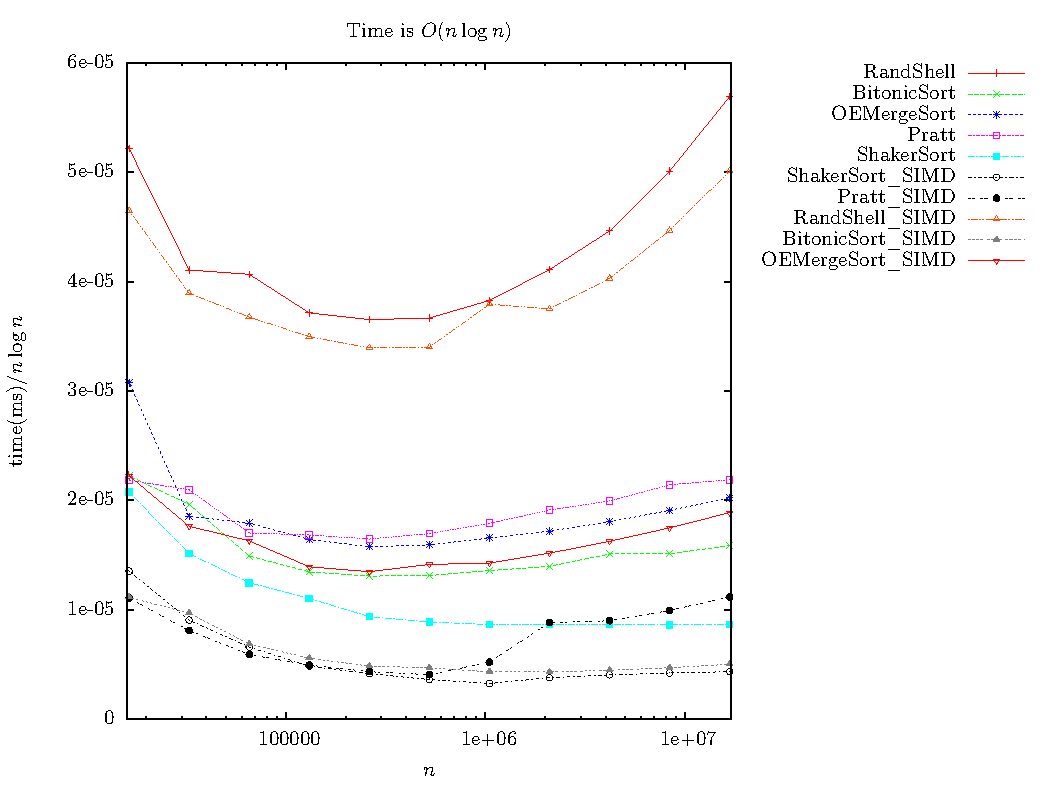
\includegraphics[width=\textwidth]{graphs/SIMD/nlogntime.pdf}
\caption{Time with and without SIMD}
\label{fig:SIMD:time}
\end{figure}


\begin{figure}
\center
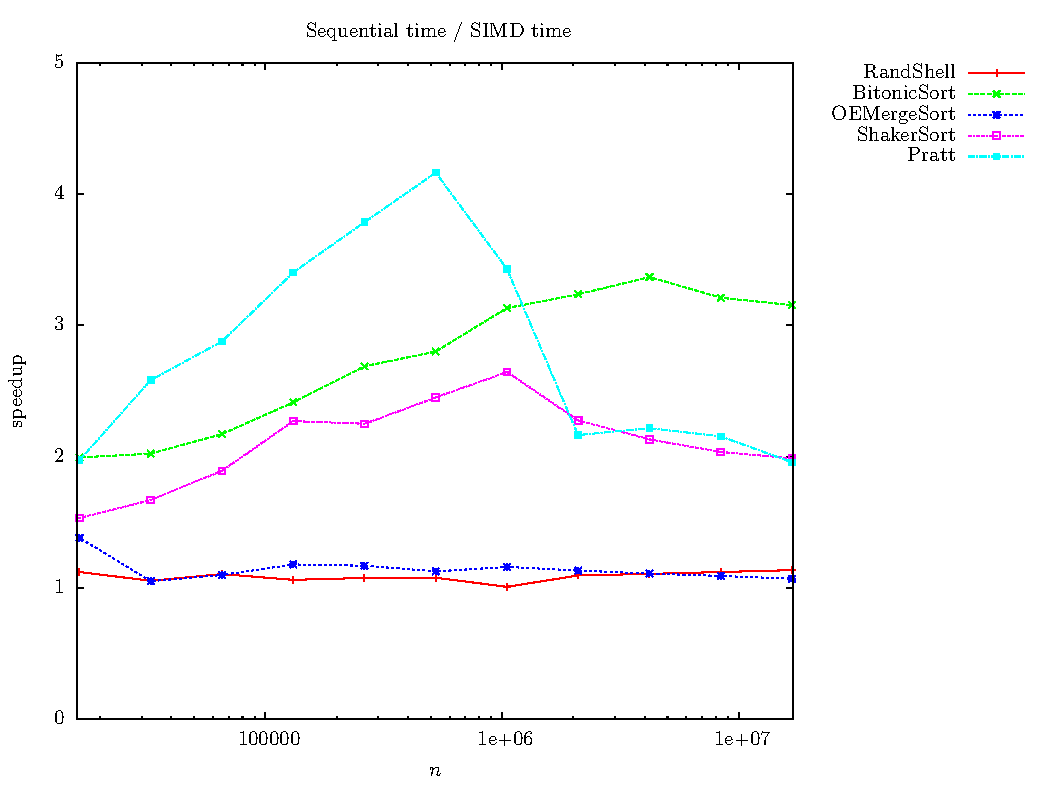
\includegraphics[width=\textwidth]{graphs/SIMD/timediff.pdf}
\caption{Time factor with and without SIMD}
\label{fig:SIMD:timediff}
\end{figure}



\FloatBarrier
\section{CUDA Experiments}

Section~\ref{sec:CUDAImpl} discusses the possibility of using CUDA to enable GPU-assisted execution of sorting networks, to speed up their computations through massive parallelism. This section shows the actual results of moving large parts of the program to the GPU, and examines how much of a speed gain is attainable both on old and new GPUs.

Programs were run on the machine described in Section 5.1, featuring a graphics card that is targeted at professional GPU-intensive applications, but is rather dated, and on a newer machine featuring a modern GPU targeted at computer gaming.

The newer machine has the following specifications:

\begin{description}
\item[CPU:] Intel i7-4810MQ, 2.8GHz, 6 MB Cache
\item[RAM:] 8GB
\item[GPU:] NVIDIA GeForce GTX 870M 
\item[Operating System:] Ubuntu 14.04 LTS
\end{description}

All CUDA implementations were separately compiled objects, and linked into the main program, to preserve sequential behaviour when CUDA is not in use. The CUDA objects were written in CUDA C++, and compiled with the following additional parameters, parameters separated by slashes varied between GPU architectures.

\begin{description}
\item[\texttt{-O3}] Use the highest optimization level
\item[\texttt{-arch=compute\_12 / -arch=compute\_30}] Optimize compilation for the specified architecture.
\item[\texttt{-code=sm\_12 / code=sm\_30}] Optimize code generation for the specified architecture.
\item[\texttt{-{}-maxregcount 16}] Use a maximum of 16 registers per thread, allowing full occupancy for all cards from CUDA 1.2 and up. 
\end{description}


\subsection{Improvements in Running Time}

Since we are now comparing different architectures, it makes little sense to consider hardware-specific metrics such as branch mispredictions and cache misses, so let us instead focus entirely on the running time, and what gains can be made by offloading parts of the program to the GPU.

Figure~\ref{fig:CUDAQuadro:time} and~\ref{fig:CUDAGTX:time} show the running time of the different algorithms when using CUDA on the different architectures.
There are three main things to notice in these, independent of the graphics cards. Firstly, Randomized Shellsort has a much better time handling cache misses when using the GPU, since we offload the random memory accesses to the GPU, and since the GPU has a much higher memory bandwith than the GPU, it seems to cope better with these access patterns.
Secondly, the other CUDA-assisted algorithms all seem to perform well, and even seem to have a running time that is close to $O(n \log n)$ in practice when they can use the GPU for massively parallel computations.
Finally, CUDA-based Bitonic Sort outperforms all other algorithms on the chart. This shows the power of migrating the entire algorithm to the GPU, and properly utilizing the memory manipulation options of the CUDA architecture.

\begin{figure}
\center
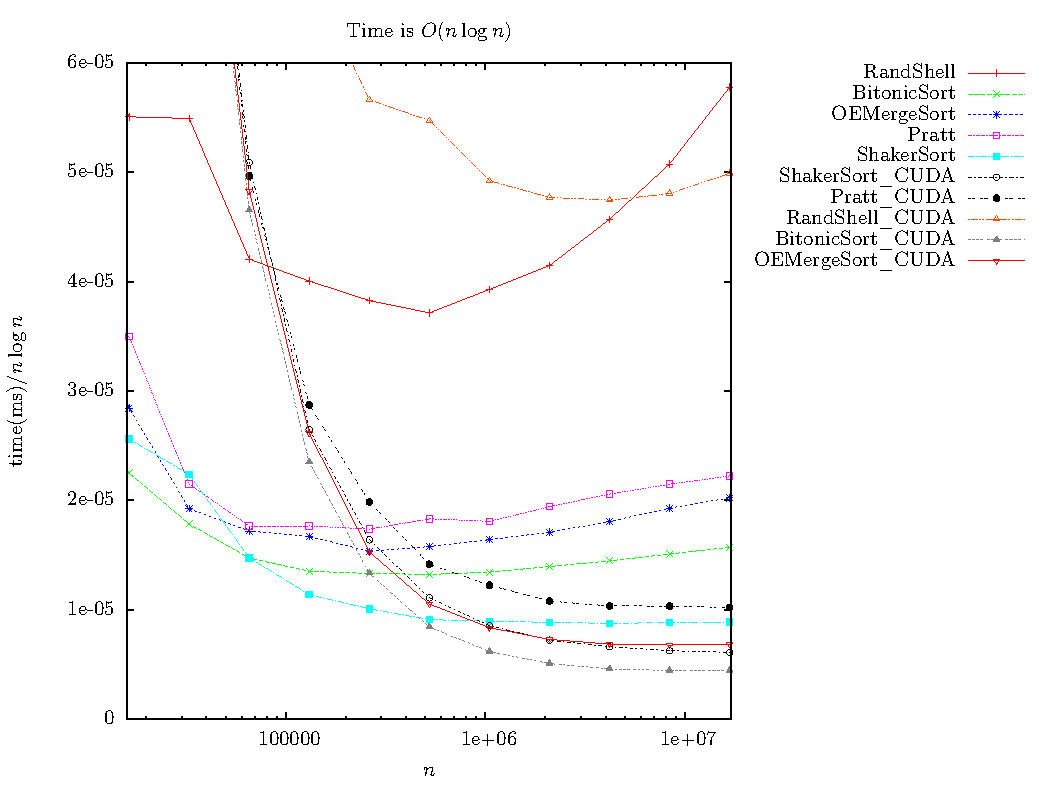
\includegraphics[width=\textwidth]{graphs/CUDA/nlogntime.pdf}
\caption{Time with and without CUDA, Quadro FX 880M}
\label{fig:CUDAQuadro:time}
\end{figure}


\begin{figure}
\center
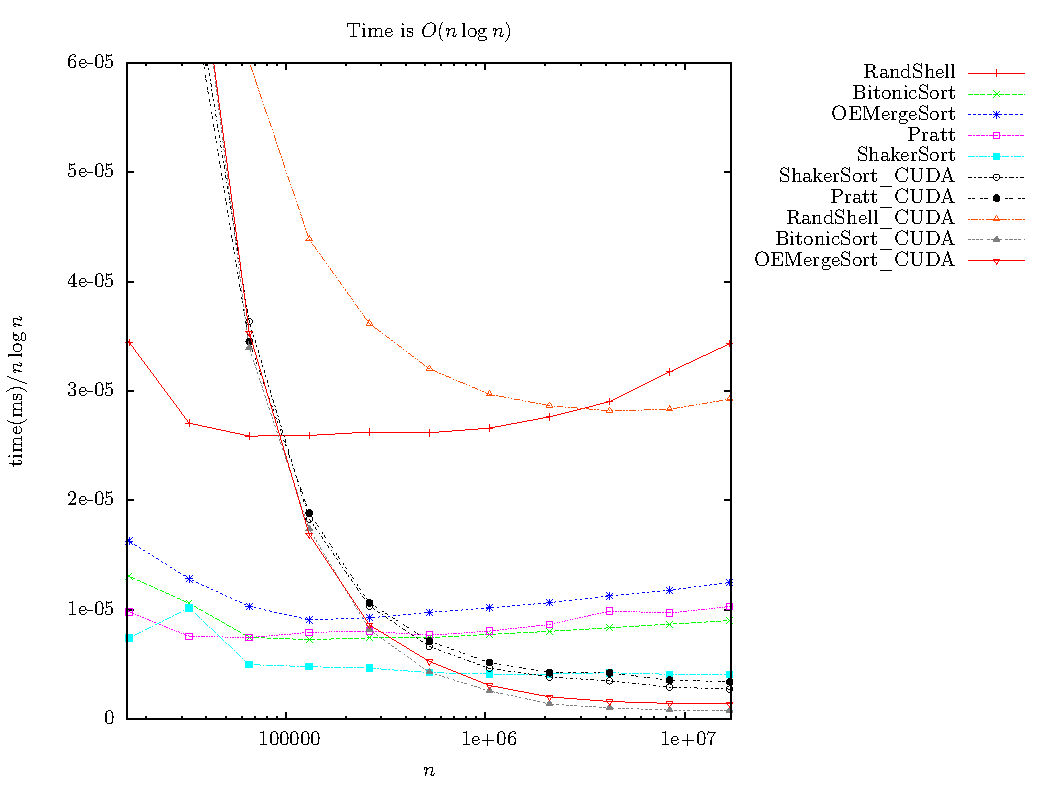
\includegraphics[width=\textwidth]{graphs/CUDAHueg/nlogntime.pdf}
\caption{Time with and without CUDA, GTX 870M}
\label{fig:CUDAGTX:time}
\end{figure}


In fact, let us further expand the view of the CUDA-enabled algorithms, Randomized Shellsort excluded.

Figure~\ref{fig:CUDAQuadro:cudatime} and~\ref{fig:CUDAGTX:cudatime} shows a view of a small selection of the included algorithms, with \texttt{std::sort}. The graphs are given the same scale on the y-axis, so the running times are directly comparable.

What we see here, is that the CUDA-assisted algorithms start out relatively slow, but provide excellent scalability as the input size increases, and in fact seem to be nearing an $O(n \log n)$ running time due to the massively parallel execution. This comes as a big surprise in the case of the algorithms that would normally be $\Theta(n \log^2 n)$, as the CUDA-implementations are supposed to have similar asymptotic running times. It is hard to explain exactly how the GPU achieves this, but most likely, the GPU scales well with a large amount of threads, and the additional logarithmic factor is getting overshadowed by the GPU scaling to larger input sizes.

Most impressive of all, are the running times presented in Figure~\ref{fig:CUDAGTX:cudatime}, where we see the CUDA-assisted sorting networks thoroughly outperform \texttt{std::sort}.

\begin{figure}
\center
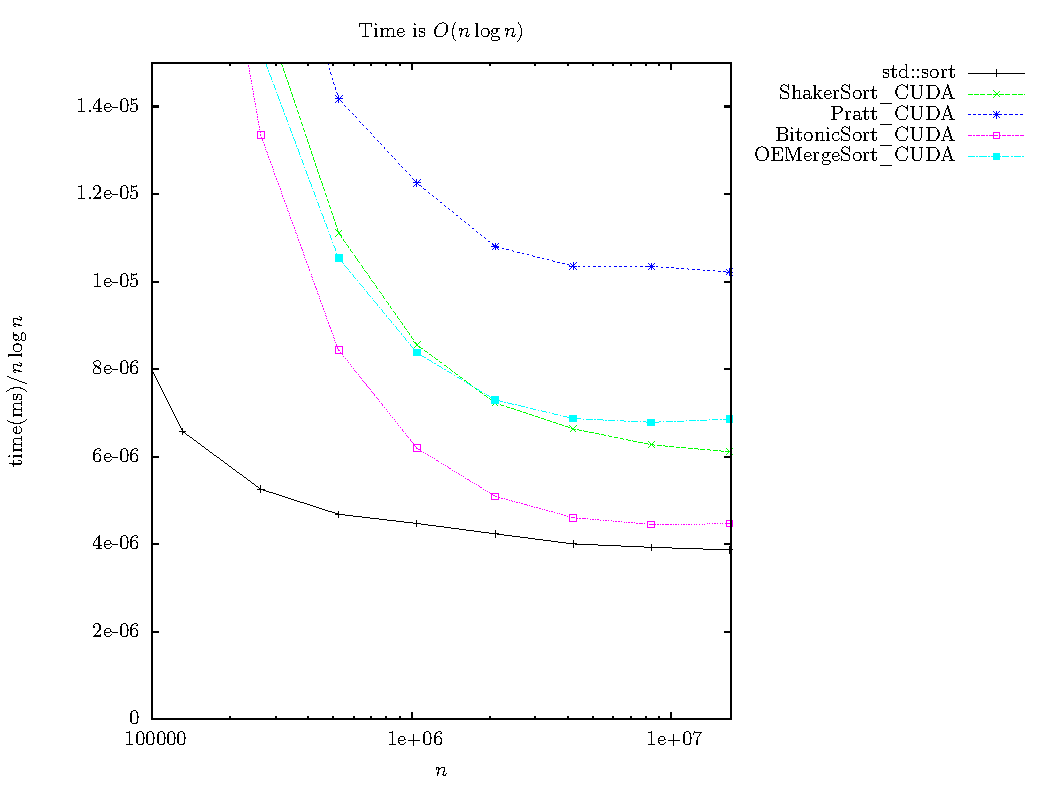
\includegraphics[width=\textwidth]{graphs/CUDA/cudatime.pdf}
\caption{Sectioned time with and without CUDA, Quadro FX 880M}
\label{fig:CUDAQuadro:cudatime}
\end{figure}

\begin{figure}
\center
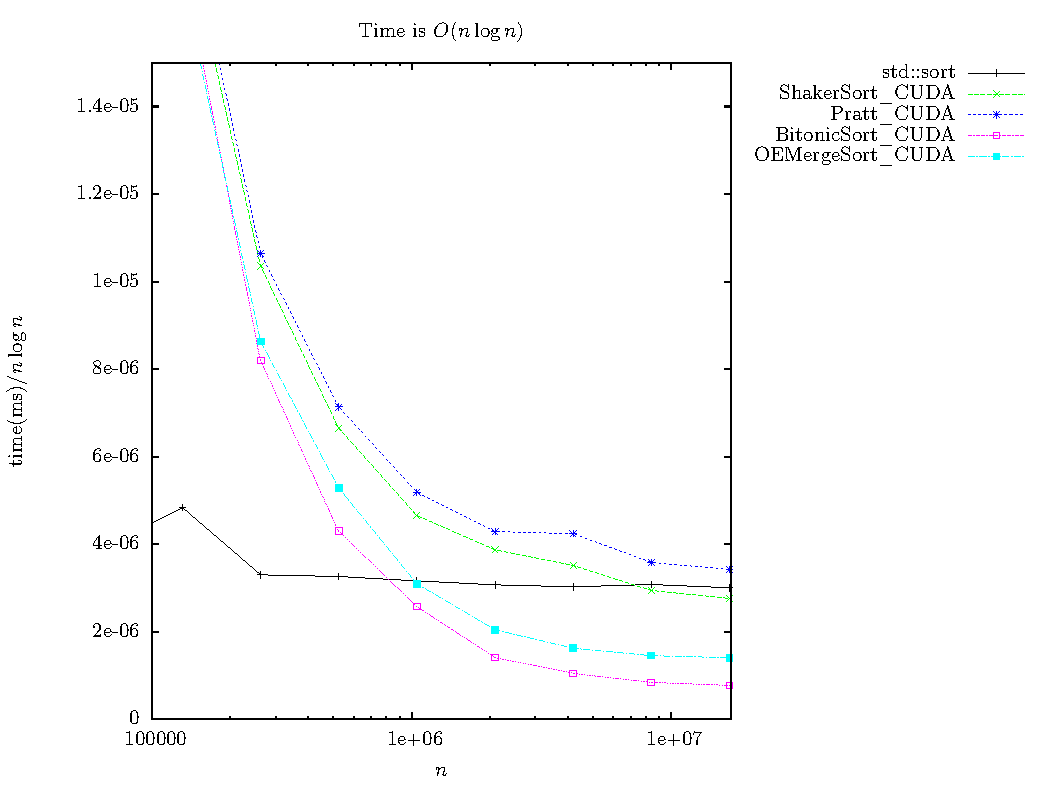
\includegraphics[width=\textwidth]{graphs/CUDAHueg/cudatime.pdf}
\caption{Sectioned time with and without CUDA, GTX 870M}
\label{fig:CUDAGTX:cudatime}
\end{figure}

Finally, let us consider how much the individual algorithms benefit from allowing CUDA-execution of certain sections. Figure~\ref{fig:CUDAQuadro:timediff} and~\ref{fig:CUDAGTX:timediff} shows the factor with which we can reduce the running times of the algorithms depending on the graphics card.

For Randomized Shellsort, we see a small but noticeable gain when input sizes grow, which can be explained by the work sharing between GPU and CPU. Note that the GPU-assisted verison of Randomized Shellsort does not seem to be impacted as heavily by the cache limit as as the seqeuntial one.

For the Shellsort variants, we see a respectable gain. This gain is caused by the adaptability of h-shakes on the GPU, as these exhibit both excellent parallelism, but also good memory access patterns. The Shellsort variants do however suffer from not having their entire execution moved to the GPU. Note that Pratt's Shellsort benefits more from GPU-acceleration than Shaker sort, which might be due to either having a larger amount of high-distance h-shakes, or simply being slightly slower on the CPU.

The last algorithms, Bitonic Sort and Odd-Even Mergsort shows massive gains from applying CUDA execution. This is due to being moved to the GPU in their entirety, and having excellent adaptability to parallelism. The newer graphics card show an exceptional performance gain compared to the specialized card from the older machine. Note that the slightly larger gain to Bitonic sort compared to Odd-Even Mergesort due to the utilization of thread-local memory.

\begin{figure}
\center
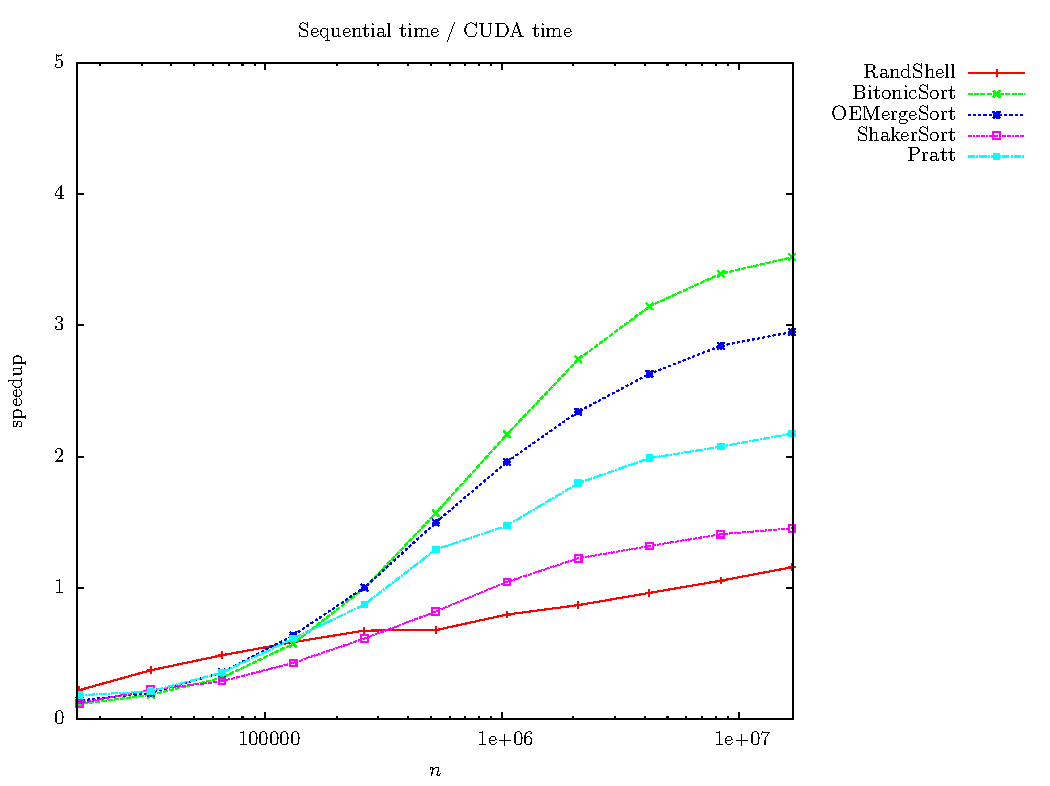
\includegraphics[width=\textwidth]{graphs/CUDA/timediff.pdf}
\caption{Time factor with and without CUDA, Quadro FX 880M}
\label{fig:CUDAQuadro:timediff}
\end{figure}

\begin{figure}
\center
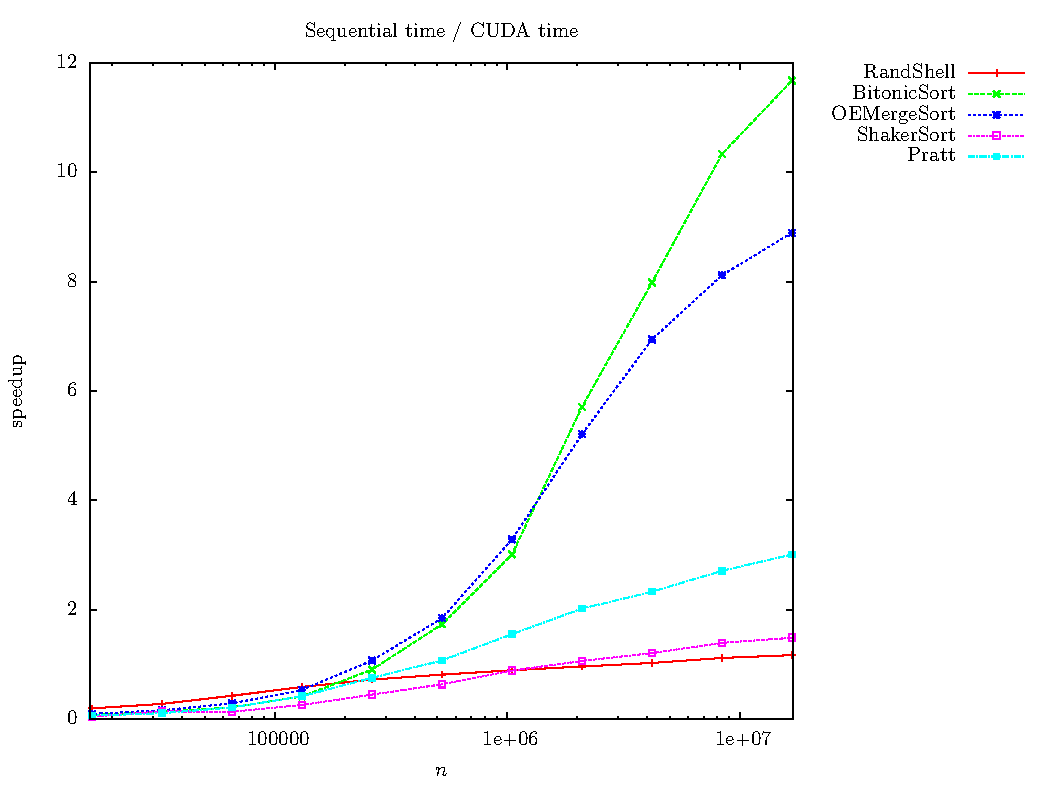
\includegraphics[width=\textwidth]{graphs/CUDAHueg/timediff.pdf}
\caption{Time factor with and without CUDA, GTX 870M}
\label{fig:CUDAGTX:timediff}
\end{figure}

\subsection{Experiment Conclusion}

The experiment showed that many of the algorithms benefit well from GPU-assisted execution, but the amount of speed-up gained varies widely between the different algorithms.

We've seen that with the $\Theta(n \log^2 n)$ algorithms, the GPU-parallelism seems the somehow make up for the additional logarithmic factor in execution time, and make these algorithms approach an $O(n \log n)$ running time in practise.

Especially the classic sorting networks of~\citeA{SNApplications} show a great suitability for GPU sorting, and even beats \texttt{std::sort} on modern hardware.

\FloatBarrier
\section{OpenMP Experiments}
\label{sec:OMPExperiments}

Section~\ref{sec:OMP} describes the possibility of OpenMP-assisted multi-threading in most of the data-oblivious sorting algorithms used in this thesis. In that section, we also describe how each individual algorithm has been modified in order to support classical multi-threading.

In this set of experiments we extend our findings with experimental data showing the impacts of multi-threading.

Keep in mind that the \texttt{Intel i7-M620}, is a dual-core CPU using hyper-threading, which gives us two physical cores, able to run four simultaneous threads. This should give us an upper limit on the speed-up achieved to be four, but in practise this will be far from achievable. 

The setups of the algorithms are identical to those of Section~\ref{sec:Performance} and~\ref{sec:ShellsortExperiments}. Annealing Sort is not included, due to being highly serial.

\subsection{Running Time}

\begin{figure}
\center
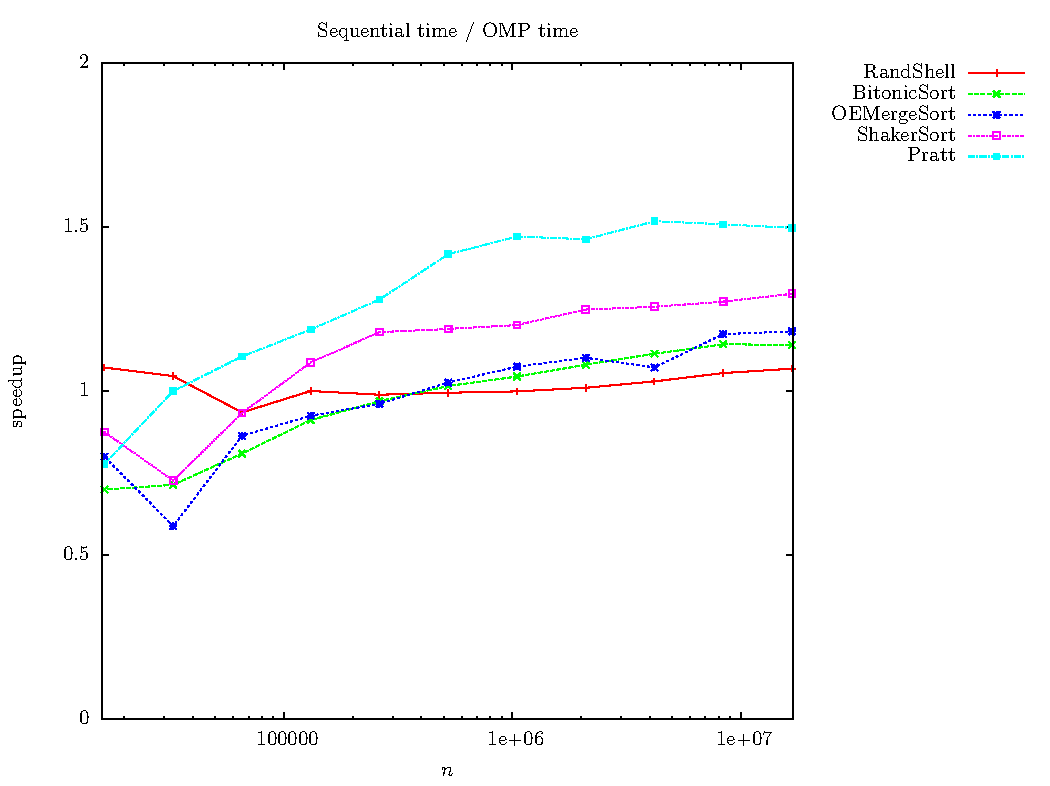
\includegraphics[width=\textwidth]{graphs/OMP/timediff.pdf}
\caption{Running Time improvement by OpenMP application}
\label{fig:OMP:timediff}
\end{figure}

Let us start by looking at the actual running time of the algorithms.
Figure~\ref{fig:OMP:timediff} shows the factor gained in execution speed when OpenMP is applied, as a measure of wall-clock time for each algorithm. The value for the largest input size is shown are collected in Table~\ref{tab:OMP:timedifffinal}.

\begin{table}[!h]
\begin{adjustwidth}{-.5in}{-.5in}
\centering
\begin{tabular}{|l|c|c|c|c|c|}
\hline
Algorithm & Randomized Shellsort & Bitonic Sort & Odd-Even Mergesort & Pratt & Shaker Sort \\ \hline
Factor    & 1.07                 & 1.14         & 1.18 & 1.50 & 1.29           \\ \hline
\end{tabular}
\caption{OpenMP gain for largest input size, $2^24$}
\label{tab:OMP:timedifffinal}
    \end{adjustwidth}
\end{table} 

Randomized Shellsort gets a small improvement from multi-threading, since some parts of the algorithm can be executed in parallel, though a great deal synchronization is required.

Both Bitonic Sort and Odd-Even Mergesort show a better application of multi-threading, and achieve a higher improvement in running time, due to the recursive calls adapting well to the task-based methodology of OpenMP.

Finally we see the two normal Shellsort variants both achieve a substantial  improvement in running time by using OpenMP. This great benefit of multi-threading in the simple Shellsort variants stems from the intrinsic separation of sub-sequences in the algorithms. Pratt's Shellsort impressively tops the chart by having many sub-sequences that divide evenly into the amount of threads, and handling these in a simpler manner than Shaker Sort.

These running times all show that we are far from even utilizing both cores fully, and even further from the 4-factor speedup that might be possible when fully utilizing hyper-threading. Let us further investigate why we are not anywhere near maximum utilization.

\subsection{Instructions, Cache Misses and Branch Mispredictions}

\begin{figure}
\center
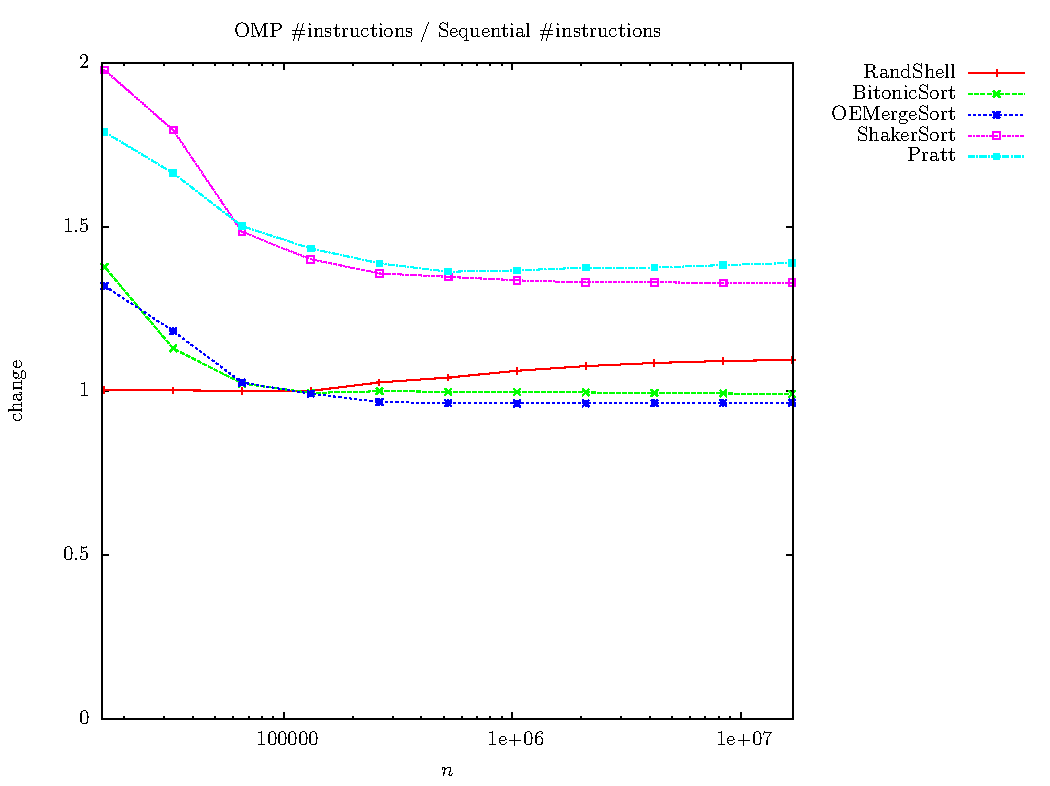
\includegraphics[width=\textwidth]{graphs/OMP/instrdiff.pdf}
\caption{Instruction degradation by OpenMP application}
\label{fig:OMP:instrdiff}
\end{figure}

\begin{figure}
\center
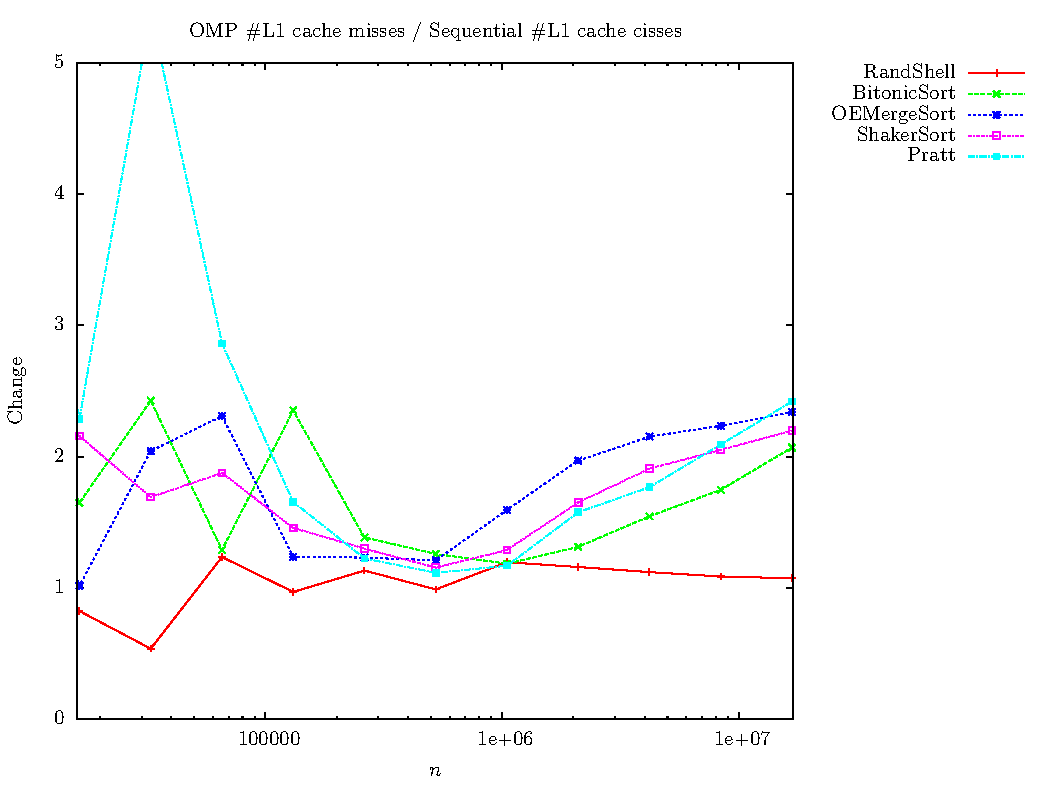
\includegraphics[width=\textwidth]{graphs/OMP/cachediff.pdf}
\caption{Cache degradation by OpenMP application}
\label{fig:OMP:cachediff}
\end{figure}

\begin{figure}
\center
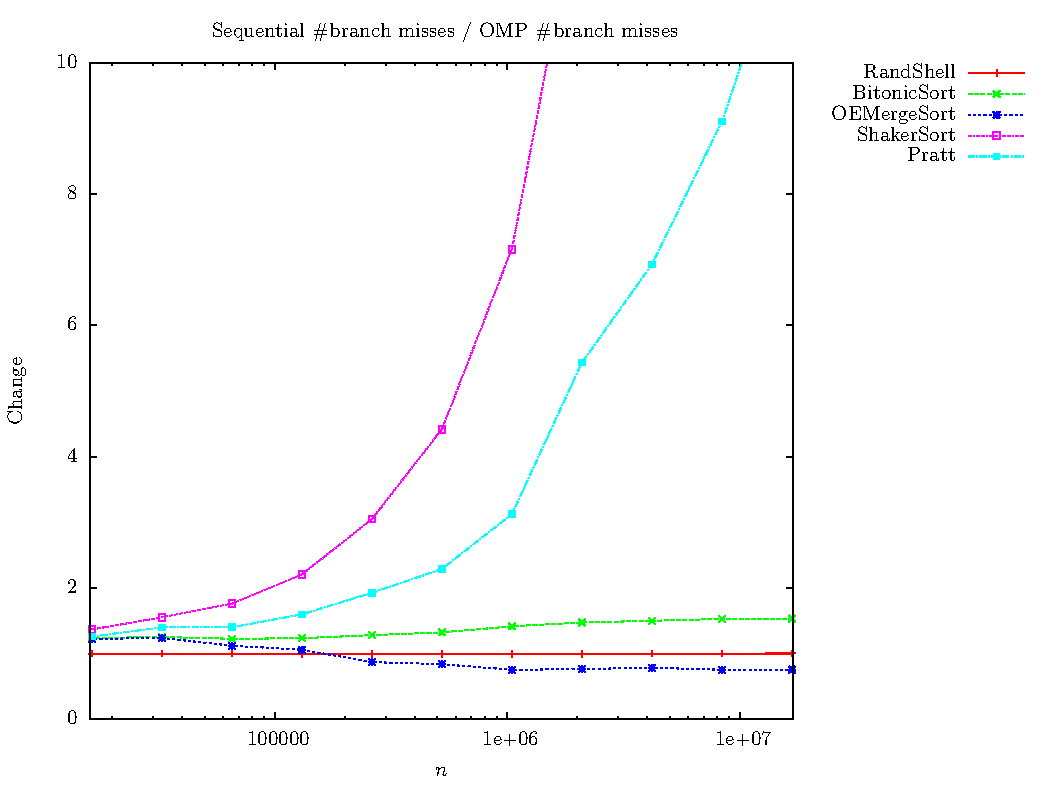
\includegraphics[width=\textwidth]{graphs/OMP/branchdiff.pdf}
\caption{Branch degradation by OpenMP application}
\label{fig:OMP:branchdiff}
\end{figure}

In order to explain the non-optimal utilization of CPU time, we must study the low-level hardware characteristics.

Instructions are a major factor in execution time, and each type of algorithm is affected differently when applying multi-threading.
Randomized Shellsort sees a slightly increased instruction count due to threading overhead, but the high baseline instruction count keeps this impact low. 
Bitonic Sort and Odd-Even Mergesort both see a minor effect from multi-threading, and there is even a reduction in instructions. This effect is strange, but is likely due to the low instruction overhead of OpenMP tasks, and some compiler magic
\footnote{Compilation is done using \texttt{Ofast}, which favours speed over executable size, which may have an adverse effect on instruction count.}.
Finally, we see Pratt's Shellsort and Shaker Sort having a high instruction overhead, due to complicated threading control, and a low baseline.

For the L1 cache misses, we see Randomized Shellsort having a small increase, due to a high baseline. The other algorithms show a moderate increase in L1 cache misses due to data sharing between the CPU cores.

In branch misses, we see almost no increase for Randomized Shellsort, due to a high baseline. Bitonic Sort increases slightly, due to thread synchronization, while Odd-Even Mergesort strangely decreases \footnote{
Explaining a decrease in branch mispredictions when applying multi-threading is difficult. Possible causes might be changes in the inlining strategy, or a collision in prediction counters when operating in single-threaded mode. Alternatively, having each recursive call separated to a single thread might prevent mispredictions across calls.
}. The two variants of Shellsort see major increase in branch mispredictions, due to having a great amount of logic applied in the scheduling of threads, and a low baseline.

\subsection{Experiment Conclusions}

This set of experiments shows that OpenMP is a viable strategy for improving the performance of data-oblivious sorting algorithms, though not nearly as effective as SIMD and CUDA. We also identify several performance issues keeping the OpenMP implementation from achieving the maximum possible performance gain.


\FloatBarrier
\section{Experimental Results Summary}

As a concluding figure for this chapter, we present Table~\ref{tab:algtimes}, that shows the execution time, in seconds, for each algorithm and optimization scheme for the largest available input size. Each algorithm has had the fastest optimization scheme marked in bold.
Note that the OpenMP results are slightly skewed towards a higher value than that of the other optimization schemes, as the high-precision CPU-time clock is not applicable to multi-threading.

\begin{table}[!h]
\centering
\begin{tabular}{|l|c c c c|}
\showrowcolors
\hline
& Base & SIMD & CUDA & OpenMP  \\ \hline
Randomized Shellsort & 22.6 & 20.2 & \textbf{20.1} & 21.5\\ 
Bitonic Sort & 6.41 & 2.02 & \textbf{1.80} & 5.61\\ 
Odd-Even Mergesort & 8.15 & 7.60 & \textbf{2.76} & 7.02\\ 
Pratt's Shellsort & 8.82  & 4.50 & \textbf{4.11} & 5.85 \\ 
Shaker Sort & 3.48 & \textbf{1.75} & 2.46 & 2.65\\ 
Annealing Sort & \textbf{67.3} & - & - & - \\ \hline
\end{tabular}
\caption{Algorithm performance overview}
\label{tab:algtimes}

\end{table} 

%%%%%%%%%%%%%%%%%%%%%%%%%%%%%%%%%%%%%%%%%%%%%%%%%%%%%%%%%%%%%%%%%%%%%%%

\chapter{Conclusion}
\label{ch:conclusion}

\section{General Conclusions}

In this thesis we have shown that data-oblivious sorting algorithms, despite often being confined either hardware or theory, can easily be implemented in software while still maintaining both their data-oblivious properties and having running times that are entirely reasonable.

We also find that several new developments in hardware greatly benefit the performance of data-oblivious sorting networks, as they often contain high levels of parallelism. Especially impressive is the performance of classic sorting networks when properly modified to fully utilize the GPU, where they can achieve running times beneath that of the highly optimized sorting algorithm provided by the \texttt{C++} standard library.

Two common problems for data-oblivious sorting algorithms appear to be cache misses and sub-optimal asymptotical instruction counts. Most likely we will see these algorithms improve, as hardware developments focuses on larger caches as opposed to clock frequency, the problem of cache misses might be diminished, while the algorithms showing sub-optimal instruction counts can be migrated to the GPU, where large improvements in pure processing power is still occurring.

Preliminary results for automatic vectorization techniques show promising results in reducing the amount of operations required to execute sorting data-oblivious sorting algorithms, though modern compilers are still not up to the task of recognising sorting networks in order to apply the required transformations.

In short, the work of this thesis should show that data-oblivious sorting networks, while they might have some problems when implemented in a straight-forward sequential manner, are still entirely relevant due to modern hardware developments.

\section{Further Work}

Due to the broad coverage of algorithms and optimization techniques covered in this thesis, there are a significant number of subjects left open for further research.

The automatic vectorization and reordering techniques of Chapter~\ref{ch:SIMDerize} could be implemented as a compiler module or an extension to an existing language runtime in order to test the actual effectiveness. This would allow for comparisons with already existing techniques, and enable collection of data both on the performance and detection rate of automatic vectorization.

Several additional algorithms could be included in the experiments, including the Pariwise Sorting network of~\citeA{PeriodicSortingNetwork} and the Pairwise Sorting network~\citeA{PairwiseSorting} are both easy to implement on modern hardware and might prove to be efficient in practice. The reduced number of comparisons achieved in~\citeA{DivideSortMerge} might prove to have a beneficial effect on performance and experimenting with a greater amount of merging sequences could give interesting results.

The optimization techniques presented in Chapter~\ref{ch:Implementations} are implemented and tested separately, but it might be beneficial to combine some of these techniques. When subproblems become too small for efficient CUDA execution, switching to SIMD or OpenMP is a definite possibility. Additionally, many of the OpenMP-optimized algorithms still allow for SIMD operations to be used.




%%%%%%%%%%%%%%%%%%%%%%%%%%%%%%%%%%%%%%%%%%%%%%%%%%%%%%%%%%%%%%%%%%%%%%%

\addcontentsline{toc}{chapter}{Primary Bibliography}
\bibliographystyleA{plain} 
\bibliographyA{thesis}
\addcontentsline{toc}{chapter}{Secondary Bibliography}
\bibliographystyleB{plain} 
\bibliographyB{thesis} % remove this if you don't need secondary literature

\FloatBarrier
\begin{appendices}
\chapter{Shared Memory for CUDA-Based Bitonic Sort}
\label{app:CUDABSShared}
\begin{figure}
\center
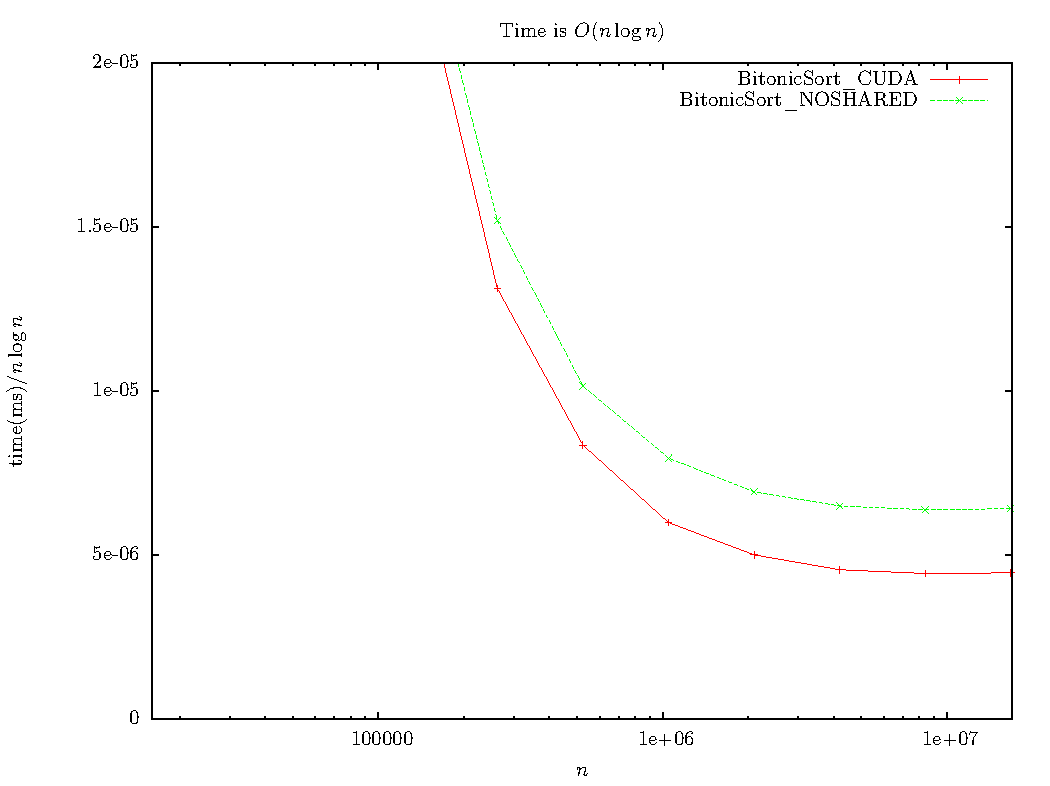
\includegraphics[width=\textwidth]{graphs/CUDAShared/nlogntime.pdf}
\caption{Running time of CUDA-based Bitonic Sort with and without shared memory, Quadro FX 880M}
\label{fig:CUDAShared}
\end{figure}
As mentioned in Section~\ref{sec:CUDAImpl}, utilizing shared memory for Bitonic Sort can be a big gain, and the graphs in the experiments section take advantage of this fact.
To further strengthen this claim, we have shown the effect of omitting the usage of shared memory in Figure~\ref{fig:CUDAShared}.

The figure clearly shows a major improvement in running time when utilizing shared memory.

\chapter{Fixed Sizes for Bitonic Sort}
\label{app:BitonicSize}
\begin{figure}
\center
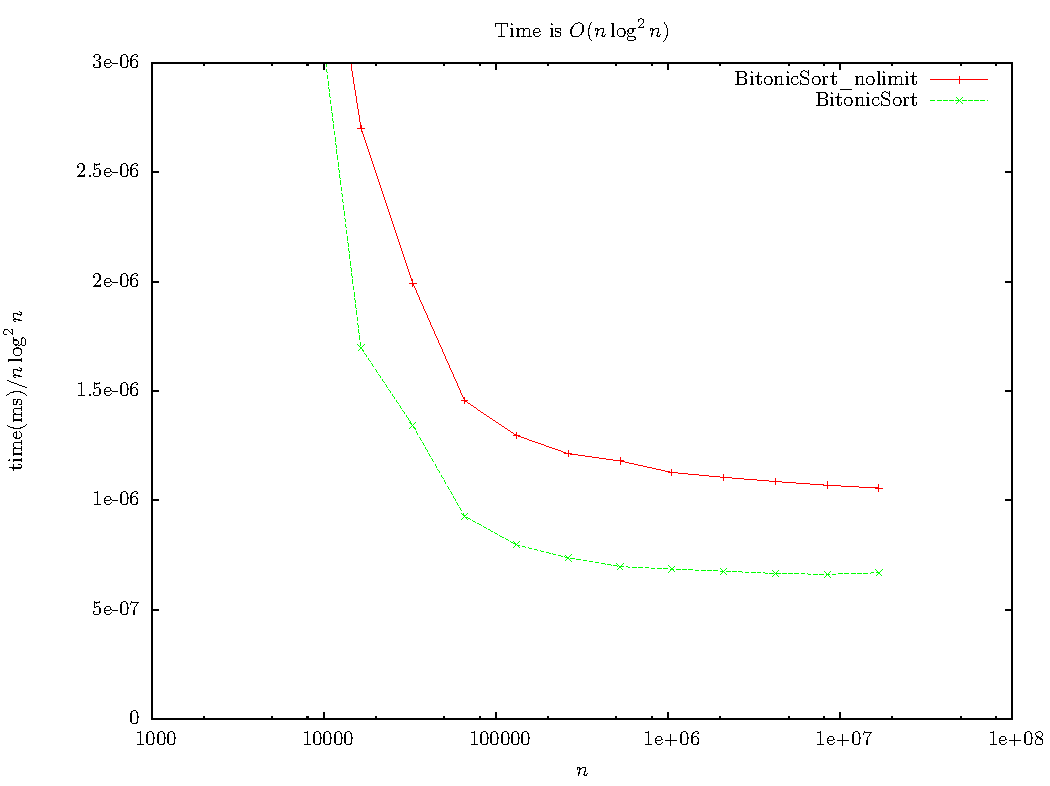
\includegraphics[width=\textwidth]{graphs/compiler/nlogntime.pdf}
\caption{Running time for Bitonic Sort, with and without fixed sizes}
\label{fig:BitonicSize}
\end{figure}
In Section~\ref{sec:BitonicImplementation} it is claimed that using fixed sizes for Bitonic Sort improves performance.

To support this claim, we have Figure~\ref{fig:BitonicSize}, that shows the optimized Bitonic sort in the experiments, compared to a version of Bitonic Sort that supports arbitrary input sizes, shown in the graph as \texttt{BitonicSort\_nolimit}.

\chapter{PRNG Effect on Performance}
\label{app:PRNG}
\begin{figure}
\center
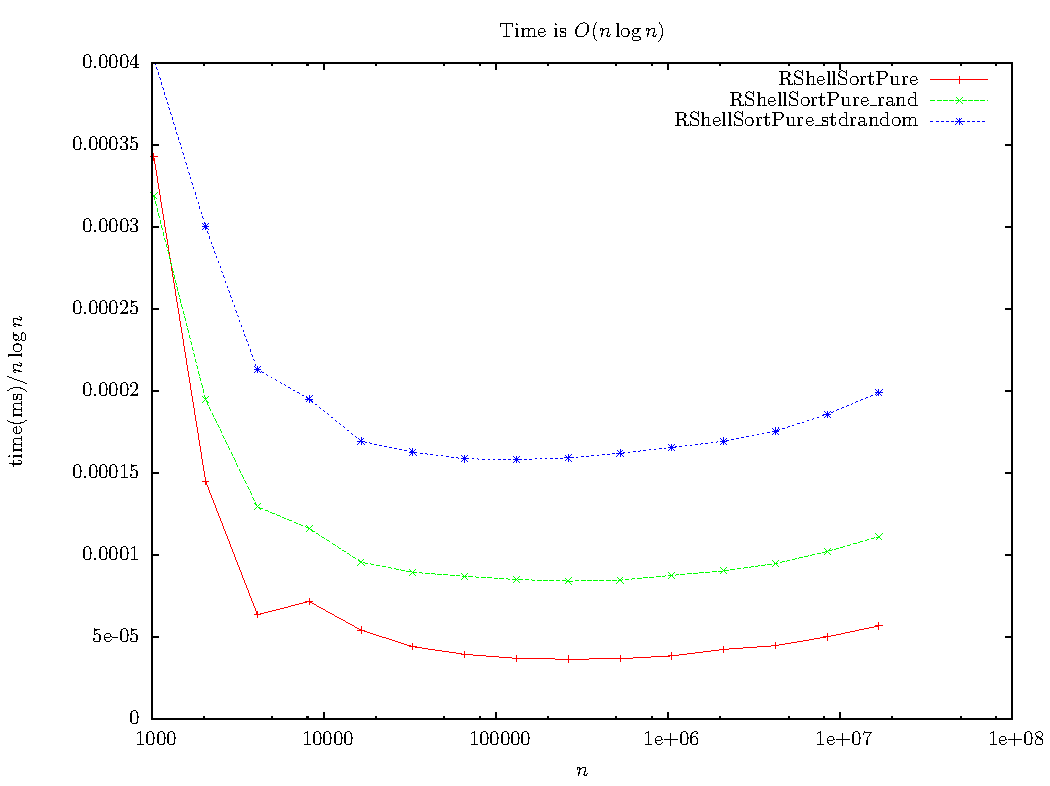
\includegraphics[width=\textwidth]{graphs/rand/nlogntime.pdf}
\caption{Running time for Randomized Shellsort, with varying PRNGs}
\label{fig:rand}
\end{figure}
Choosing a random number generator with good performance is very important for Randomized Shellsort, as noted in\ref{sec:PRNG}.

To show how big an effect the choice of PRNG actually has, which is shown in Figure~\ref{fig:rand}, where the optimized PRNG used in the experiments is compared to \texttt{rand} and \texttt{mt19937} from the \texttt{C++} standard library, shown in the graph as respectively as postfixes \texttt{\_rand} and \texttt{\_stdrandom}.
\end{appendices}


\end{document}

